% !TeX spellcheck = pt_PT2

\chapter{Esquemáticas \gls{pcb}}
\label{anexo:pcb}

\begin{figure}[H]
  \centering
  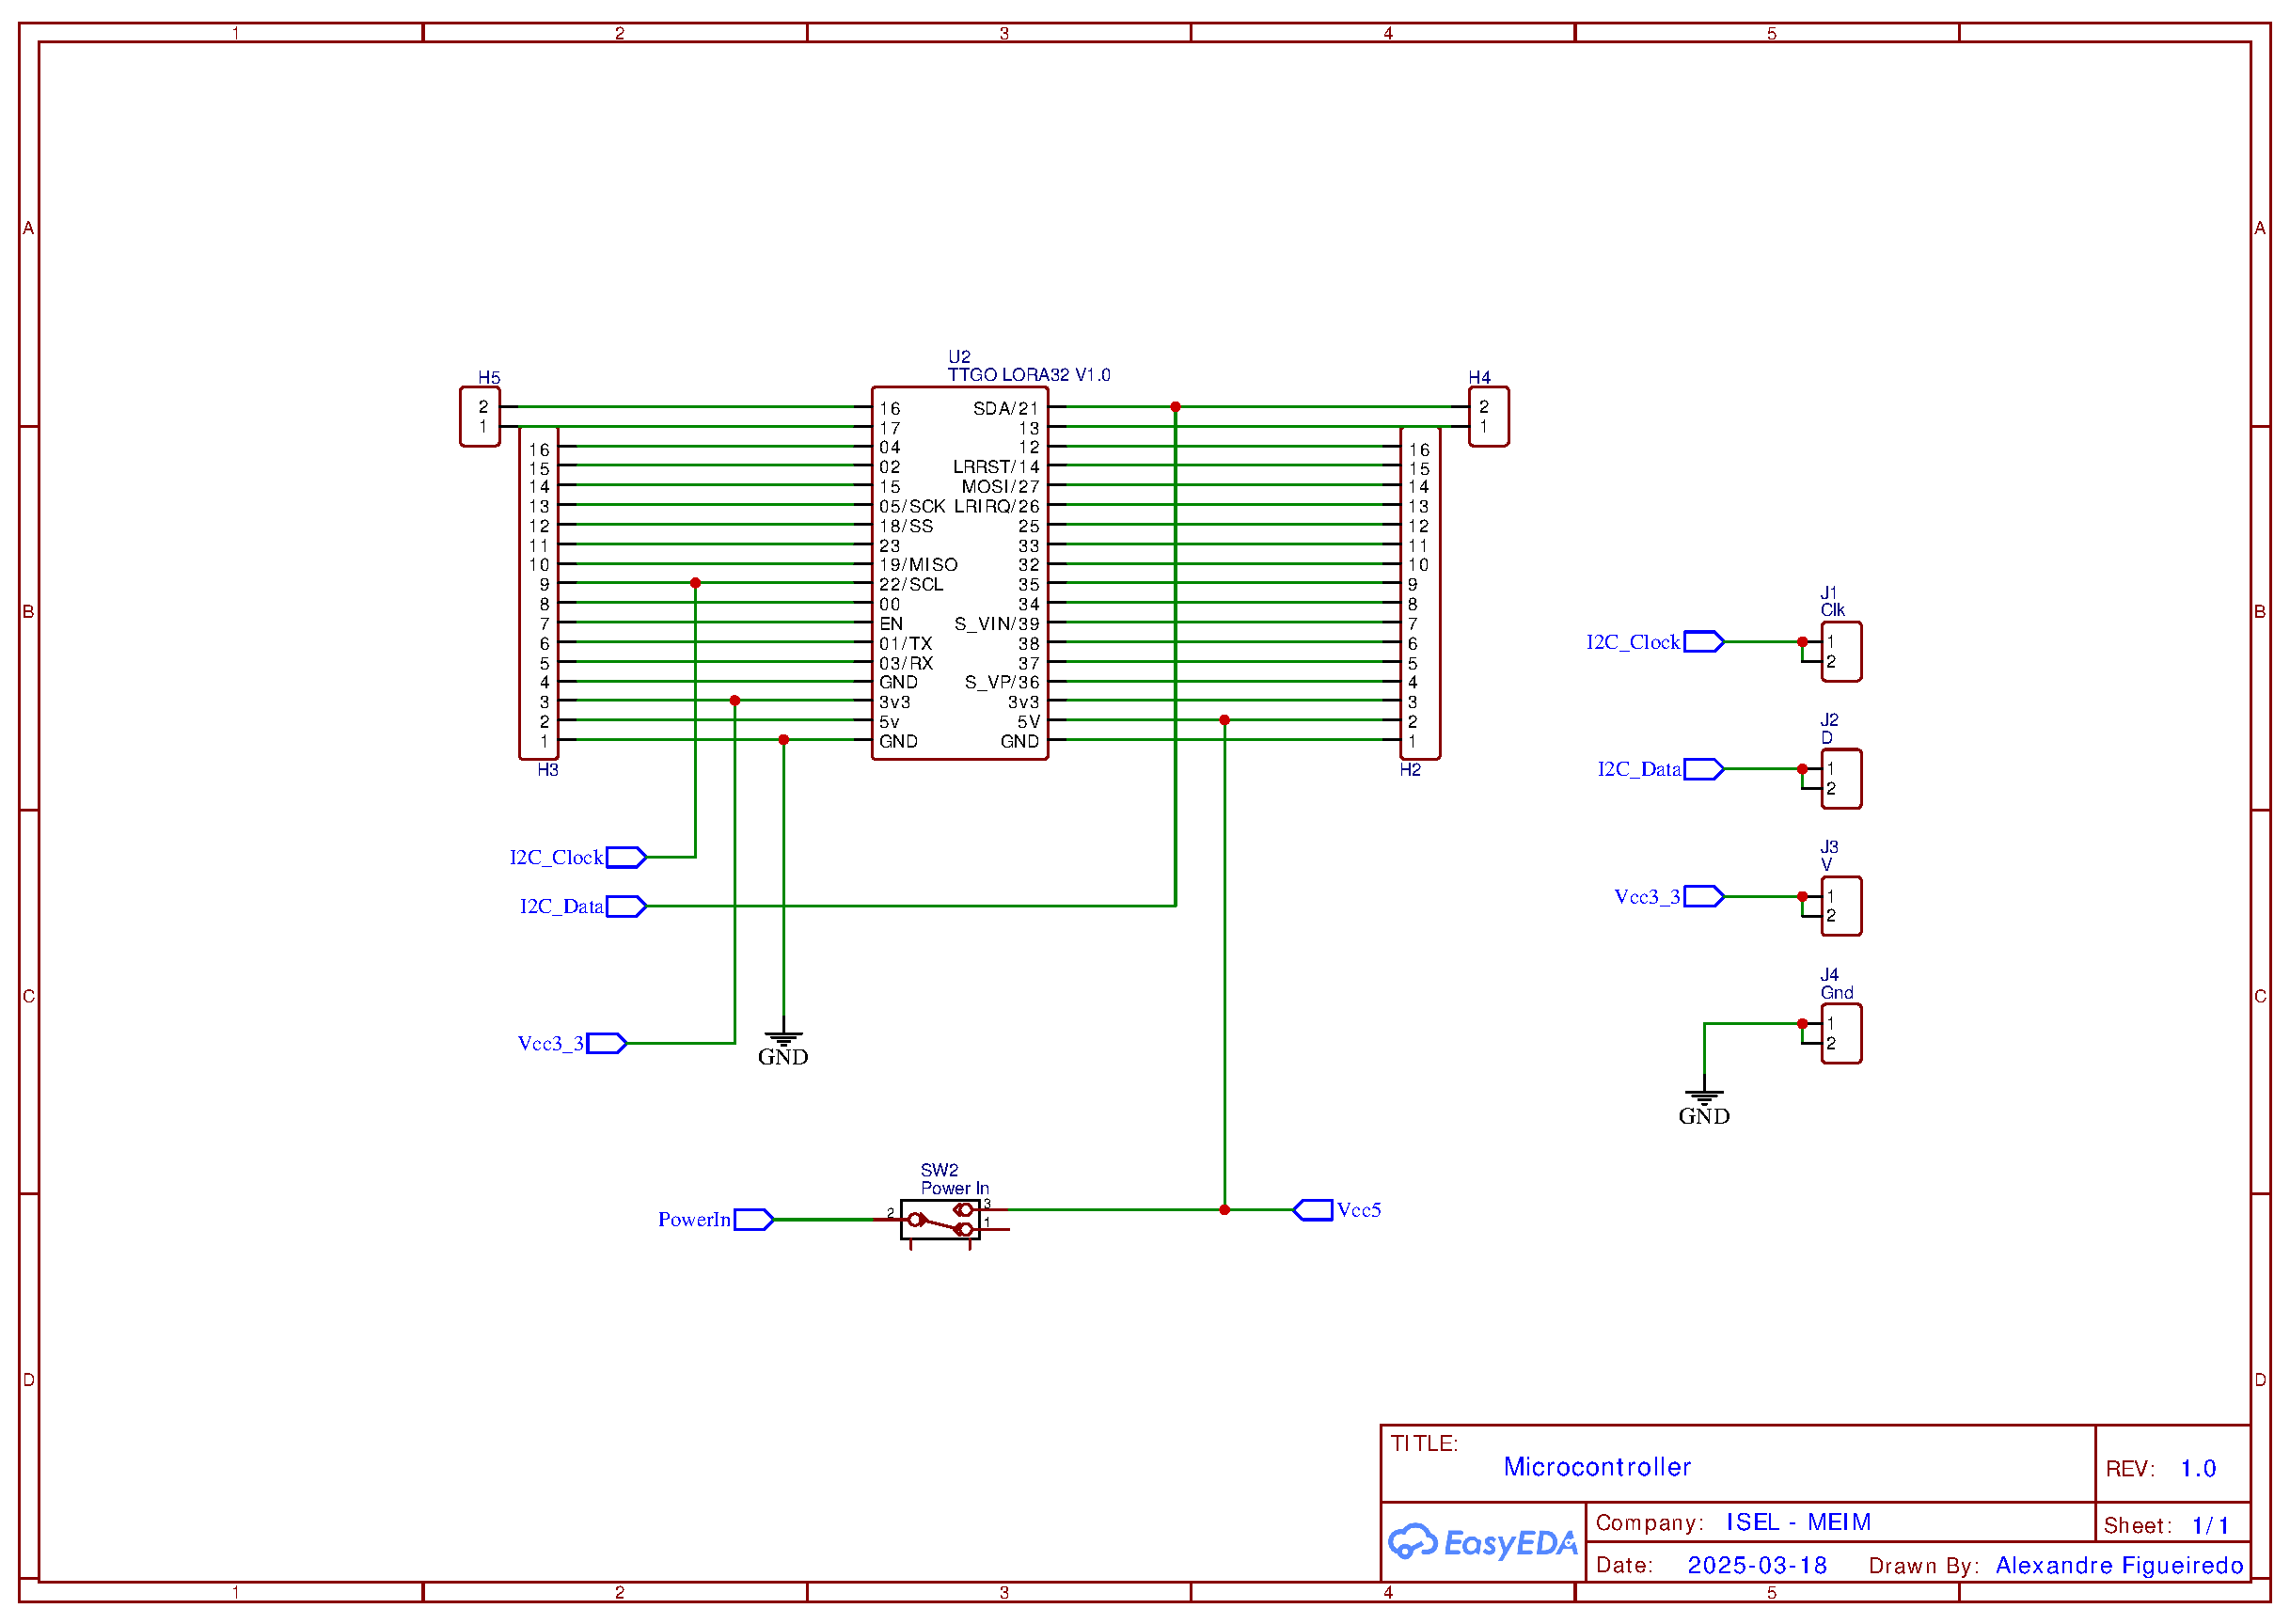
\includegraphics[page=1,width=\textwidth,height=\textheight,keepaspectratio]{anexos/esquematica.pdf}
  \caption{Esquemática do microcontrolador}
  \label{fig:esquematica-gps}
\end{figure}

\begin{figure}[H]
  \centering
  \includegraphics[page=2,width=\textwidth,height=\textheight,keepaspectratio]{anexos/esquematica.pdf}
  \caption{Esquemática dos propulsores}
  \label{fig:esquematica-props}
\end{figure}
\vspace{-0.2cm}
\begin{figure}[H]
  \centering
  \includegraphics[page=3,width=\textwidth,height=\textheight,keepaspectratio]{anexos/esquematica.pdf}
  \caption{Esquemática do \gls{imu}}}
  \label{fig:esquematica-imu}
\end{figure}

\begin{figure}[H]
  \centering
  \includegraphics[page=4,width=\textwidth,height=\textheight,keepaspectratio]{anexos/esquematica.pdf}
  \caption{Esquemática do controlo dos motores (expansor)}
  \label{fig:esquematica-expander}
\end{figure}
\vspace{-0.2cm}
\begin{figure}[H]
  \centering
  \includegraphics[page=5,width=\textwidth,height=\textheight,keepaspectratio]{anexos/esquematica.pdf}
  \caption{Esquemática do \gls{gps}}
  \label{fig:esquematica-gps}
\end{figure}

\chapter{Diagramas de classes}
\label{anexo:diagramas-de-classes}

\begin{figure}[H]
  \centering
  \resizebox{\textwidth}{!}{%
    % generated by Plantuml 1.2024.3       
\definecolor{plantucolor0000}{RGB}{255,255,255}
\definecolor{plantucolor0001}{RGB}{0,0,0}
\definecolor{plantucolor0002}{RGB}{238,238,238}
\definecolor{plantucolor0003}{RGB}{221,221,221}
\definecolor{plantucolor0004}{RGB}{204,204,204}
\definecolor{plantucolor0005}{RGB}{187,187,187}
\begin{tikzpicture}[yscale=-1
,pstyle0/.style={color=black,fill=white,line width=1.0pt}
,pstyle1/.style={color=black,line width=1.0pt}
,pstyle6/.style={color=black,fill=black,line width=1.0pt}
]
\draw[pstyle0] (794.5pt,11.602pt) -- (917.9187pt,11.602pt) arc(270:360:3.75pt)  -- (927.4187pt,36.6699pt) -- (974.5pt,36.6699pt) arc(270:360:2.5pt)  -- (977pt,349.102pt) arc(0:90:2.5pt)  -- (794.5pt,351.602pt) arc(90:180:2.5pt)  -- (792pt,14.102pt) arc(180:270:2.5pt) ;
\draw[pstyle1] (792pt,36.6699pt) -- (927.4187pt,36.6699pt);
\node at (796pt,13.602pt)[below right,color=black]{\textbf{Robot Didático}};
\draw[color=black,fill=plantucolor0002,line width=1.0pt] (13.5pt,19.602pt) -- (47.6714pt,19.602pt) arc(270:360:3.75pt)  -- (57.1714pt,44.6699pt) -- (761.5pt,44.6699pt) arc(270:360:2.5pt)  -- (764pt,117.102pt) arc(0:90:2.5pt)  -- (13.5pt,119.602pt) arc(90:180:2.5pt)  -- (11pt,22.102pt) arc(180:270:2.5pt) ;
\draw[pstyle1] (11pt,44.6699pt) -- (57.1714pt,44.6699pt);
\node at (15pt,21.602pt)[below right,color=black]{\textbf{USV}};
\draw[color=black,fill=plantucolor0003,line width=1.0pt] (404.5pt,340.602pt) -- (468.9667pt,340.602pt) arc(270:360:3.75pt)  -- (478.4667pt,365.6699pt) -- (531.5pt,365.6699pt) arc(270:360:2.5pt)  -- (534pt,473.102pt) arc(0:90:2.5pt)  -- (404.5pt,475.602pt) arc(90:180:2.5pt)  -- (402pt,343.102pt) arc(180:270:2.5pt) ;
\draw[pstyle1] (402pt,365.6699pt) -- (478.4667pt,365.6699pt);
\node at (406pt,342.602pt)[below right,color=black]{\textbf{Control}};
\draw[color=black,fill=plantucolor0004,line width=1.0pt] (601pt,428.602pt) -- (665.6727pt,428.602pt) arc(270:360:3.75pt)  -- (675.1727pt,453.6699pt) -- (722pt,453.6699pt) arc(270:360:2.5pt)  -- (724.5pt,606.102pt) arc(0:90:2.5pt)  -- (601pt,608.602pt) arc(90:180:2.5pt)  -- (598.5pt,431.102pt) arc(180:270:2.5pt) ;
\draw[pstyle1] (598.5pt,453.6699pt) -- (675.1727pt,453.6699pt);
\node at (602.5pt,430.602pt)[below right,color=black]{\textbf{Sensors}};
\draw[color=black,fill=plantucolor0005,line width=1.0pt] (181pt,303.602pt) -- (315.2991pt,303.602pt) arc(270:360:3.75pt)  -- (324.7991pt,328.6699pt) -- (325pt,328.6699pt) arc(270:360:2.5pt)  -- (327.5pt,481.102pt) arc(0:90:2.5pt)  -- (181pt,483.602pt) arc(90:180:2.5pt)  -- (178.5pt,306.102pt) arc(180:270:2.5pt) ;
\draw[pstyle1] (178.5pt,328.6699pt) -- (324.7991pt,328.6699pt);
\node at (182.5pt,305.602pt)[below right,color=black]{\textbf{Communication}};
\draw[pstyle0] (848.5pt,295.102pt) arc (180:270:5pt) -- (853.5pt,290.102pt) -- (915.8897pt,290.102pt) arc (270:360:5pt) -- (920.8897pt,295.102pt) -- (920.8897pt,330.1699pt) arc (0:90:5pt) -- (915.8897pt,335.1699pt) -- (853.5pt,335.1699pt) arc (90:180:5pt) -- (848.5pt,330.1699pt) -- cycle;
\draw[pstyle0] (860.5pt,304.6359pt) ellipse (8pt and 8pt);
\node at (860.5pt,304.6359pt)[]{\textbf{\Large C}};
\node at (871.5pt,295.102pt)[below right,color=black]{Robot};
\draw[pstyle1] (849.5pt,319.1699pt) -- (919.8897pt,319.1699pt);
\draw[pstyle1] (849.5pt,327.1699pt) -- (919.8897pt,327.1699pt);
\draw[pstyle0] (830.5pt,215.102pt) arc (180:270:5pt) -- (835.5pt,210.102pt) -- (933.7857pt,210.102pt) arc (270:360:5pt) -- (938.7857pt,215.102pt) -- (938.7857pt,250.1699pt) arc (0:90:5pt) -- (933.7857pt,255.1699pt) -- (835.5pt,255.1699pt) arc (90:180:5pt) -- (830.5pt,250.1699pt) -- cycle;
\draw[pstyle0] (842.5pt,224.6359pt) ellipse (8pt and 8pt);
\node at (842.5pt,224.6359pt)[]{\textbf{\Large C}};
\node at (853.5pt,215.102pt)[below right,color=black]{Movement};
\draw[pstyle1] (831.5pt,239.1699pt) -- (937.7857pt,239.1699pt);
\draw[pstyle1] (831.5pt,247.1699pt) -- (937.7857pt,247.1699pt);
\draw[pstyle0] (847.5pt,135.102pt) arc (180:270:5pt) -- (852.5pt,130.102pt) -- (916.7244pt,130.102pt) arc (270:360:5pt) -- (921.7244pt,135.102pt) -- (921.7244pt,170.1699pt) arc (0:90:5pt) -- (916.7244pt,175.1699pt) -- (852.5pt,175.1699pt) arc (90:180:5pt) -- (847.5pt,170.1699pt) -- cycle;
\draw[pstyle0] (859.5pt,144.6359pt) ellipse (8pt and 8pt);
\node at (859.5pt,144.6359pt)[]{\textbf{\Large C}};
\node at (870.5pt,135.102pt)[below right,color=black]{Motor};
\draw[pstyle1] (848.5pt,159.1699pt) -- (920.7244pt,159.1699pt);
\draw[pstyle1] (848.5pt,167.1699pt) -- (920.7244pt,167.1699pt);
\draw[pstyle0] (808pt,55.102pt) arc (180:270:5pt) -- (813pt,50.102pt) -- (956.4972pt,50.102pt) arc (270:360:5pt) -- (961.4972pt,55.102pt) -- (961.4972pt,90.1699pt) arc (0:90:5pt) -- (956.4972pt,95.1699pt) -- (813pt,95.1699pt) arc (90:180:5pt) -- (808pt,90.1699pt) -- cycle;
\draw[pstyle0] (820pt,64.6359pt) ellipse (8pt and 8pt);
\node at (820pt,64.6359pt)[]{\textbf{\Large C}};
\node at (831pt,55.102pt)[below right,color=black]{MotorController};
\draw[pstyle1] (809pt,79.1699pt) -- (960.4972pt,79.1699pt);
\draw[pstyle1] (809pt,87.1699pt) -- (960.4972pt,87.1699pt);
\draw[pstyle0] (27pt,63.102pt) arc (180:270:5pt) -- (32pt,58.102pt) -- (79.2148pt,58.102pt) arc (270:360:5pt) -- (84.2148pt,63.102pt) -- (84.2148pt,98.1699pt) arc (0:90:5pt) -- (79.2148pt,103.1699pt) -- (32pt,103.1699pt) arc (90:180:5pt) -- (27pt,98.1699pt) -- cycle;
\draw[pstyle0] (39pt,72.6359pt) ellipse (8pt and 8pt);
\node at (39pt,72.6359pt)[]{\textbf{\Large C}};
\node at (50pt,63.102pt)[below right,color=black]{USV};
\draw[pstyle1] (28pt,87.1699pt) -- (83.2148pt,87.1699pt);
\draw[pstyle1] (28pt,95.1699pt) -- (83.2148pt,95.1699pt);
\draw[pstyle0] (144pt,63.102pt) arc (180:270:5pt) -- (149pt,58.102pt) -- (355.9463pt,58.102pt) arc (270:360:5pt) -- (360.9463pt,63.102pt) -- (360.9463pt,98.1699pt) arc (0:90:5pt) -- (355.9463pt,103.1699pt) -- (149pt,103.1699pt) arc (90:180:5pt) -- (144pt,98.1699pt) -- cycle;
\draw[pstyle0] (156pt,72.6359pt) ellipse (8pt and 8pt);
\node at (156pt,72.6359pt)[]{\textbf{\Large C}};
\node at (167pt,63.102pt)[below right,color=black]{MovementTwoThrusters};
\draw[pstyle1] (145pt,87.1699pt) -- (359.9463pt,87.1699pt);
\draw[pstyle1] (145pt,95.1699pt) -- (359.9463pt,95.1699pt);
\draw[pstyle0] (421pt,63.102pt) arc (180:270:5pt) -- (426pt,58.102pt) -- (509.7492pt,58.102pt) arc (270:360:5pt) -- (514.7492pt,63.102pt) -- (514.7492pt,98.1699pt) arc (0:90:5pt) -- (509.7492pt,103.1699pt) -- (426pt,103.1699pt) arc (90:180:5pt) -- (421pt,98.1699pt) -- cycle;
\draw[pstyle0] (433pt,72.6359pt) ellipse (8pt and 8pt);
\node at (433pt,72.6359pt)[]{\textbf{\Large C}};
\node at (444pt,63.102pt)[below right,color=black]{Thruster};
\draw[pstyle1] (422pt,87.1699pt) -- (513.7492pt,87.1699pt);
\draw[pstyle1] (422pt,95.1699pt) -- (513.7492pt,95.1699pt);
\draw[pstyle0] (575pt,63.102pt) arc (180:270:5pt) -- (580pt,58.102pt) -- (743.0142pt,58.102pt) arc (270:360:5pt) -- (748.0142pt,63.102pt) -- (748.0142pt,98.1699pt) arc (0:90:5pt) -- (743.0142pt,103.1699pt) -- (580pt,103.1699pt) arc (90:180:5pt) -- (575pt,98.1699pt) -- cycle;
\draw[pstyle0] (587pt,72.6359pt) ellipse (8pt and 8pt);
\node at (587pt,72.6359pt)[]{\textbf{\Large S}};
\node at (598pt,63.102pt)[below right,color=black]{ThrusterController};
\draw[pstyle1] (576pt,87.1699pt) -- (747.0142pt,87.1699pt);
\draw[pstyle1] (576pt,95.1699pt) -- (747.0142pt,95.1699pt);
\draw[pstyle0] (426pt,392.102pt) arc (180:270:5pt) -- (431pt,387.102pt) -- (505.32pt,387.102pt) arc (270:360:5pt) -- (510.32pt,392.102pt) -- (510.32pt,427.1699pt) arc (0:90:5pt) -- (505.32pt,432.1699pt) -- (431pt,432.1699pt) arc (90:180:5pt) -- (426pt,427.1699pt) -- cycle;
\draw[pstyle0] (438pt,401.6359pt) ellipse (8pt and 8pt);
\node at (438pt,401.6359pt)[]{\textbf{\Large C}};
\node at (449pt,392.102pt)[below right,color=black]{Control};
\draw[pstyle1] (427pt,416.1699pt) -- (509.32pt,416.1699pt);
\draw[pstyle1] (427pt,424.1699pt) -- (509.32pt,424.1699pt);
\draw[pstyle0] (615.5pt,472.102pt) arc (180:270:5pt) -- (620.5pt,467.102pt) -- (702.093pt,467.102pt) arc (270:360:5pt) -- (707.093pt,472.102pt) -- (707.093pt,507.1699pt) arc (0:90:5pt) -- (702.093pt,512.1699pt) -- (620.5pt,512.1699pt) arc (90:180:5pt) -- (615.5pt,507.1699pt) -- cycle;
\draw[pstyle0] (627.5pt,481.6359pt) ellipse (8pt and 8pt);
\node at (627.5pt,481.6359pt)[]{\textbf{\Large C}};
\node at (638.5pt,472.102pt)[below right,color=black]{GPSData};
\draw[pstyle1] (616.5pt,496.1699pt) -- (706.093pt,496.1699pt);
\draw[pstyle1] (616.5pt,504.1699pt) -- (706.093pt,504.1699pt);
\draw[pstyle0] (614.5pt,552.102pt) arc (180:270:5pt) -- (619.5pt,547.102pt) -- (703.2492pt,547.102pt) arc (270:360:5pt) -- (708.2492pt,552.102pt) -- (708.2492pt,587.1699pt) arc (0:90:5pt) -- (703.2492pt,592.1699pt) -- (619.5pt,592.1699pt) arc (90:180:5pt) -- (614.5pt,587.1699pt) -- cycle;
\draw[pstyle0] (626.5pt,561.6359pt) ellipse (8pt and 8pt);
\node at (626.5pt,561.6359pt)[]{\textbf{\Large C}};
\node at (637.5pt,552.102pt)[below right,color=black]{IMUData};
\draw[pstyle1] (615.5pt,576.1699pt) -- (707.2492pt,576.1699pt);
\draw[pstyle1] (615.5pt,584.1699pt) -- (707.2492pt,584.1699pt);
\draw[pstyle0] (225pt,347.102pt) arc (180:270:5pt) -- (230pt,342.102pt) -- (275.04pt,342.102pt) arc (270:360:5pt) -- (280.04pt,347.102pt) -- (280.04pt,382.1699pt) arc (0:90:5pt) -- (275.04pt,387.1699pt) -- (230pt,387.1699pt) arc (90:180:5pt) -- (225pt,382.1699pt) -- cycle;
\draw[pstyle0] (237pt,356.6359pt) ellipse (8pt and 8pt);
\node at (237pt,356.6359pt)[]{\textbf{\Large C}};
\node at (248pt,347.102pt)[below right,color=black]{Led};
\draw[pstyle1] (226pt,371.1699pt) -- (279.04pt,371.1699pt);
\draw[pstyle1] (226pt,379.1699pt) -- (279.04pt,379.1699pt);
\draw[pstyle0] (219.5pt,427.102pt) arc (180:270:5pt) -- (224.5pt,422.102pt) -- (280.3588pt,422.102pt) arc (270:360:5pt) -- (285.3588pt,427.102pt) -- (285.3588pt,462.1699pt) arc (0:90:5pt) -- (280.3588pt,467.1699pt) -- (224.5pt,467.1699pt) arc (90:180:5pt) -- (219.5pt,462.1699pt) -- cycle;
\draw[pstyle0] (231.5pt,436.6359pt) ellipse (8pt and 8pt);
\node at (231.5pt,436.6359pt)[]{\textbf{\Large C}};
\node at (242.5pt,427.102pt)[below right,color=black]{LoRa};
\draw[pstyle1] (220.5pt,451.1699pt) -- (284.3588pt,451.1699pt);
\draw[pstyle1] (220.5pt,459.1699pt) -- (284.3588pt,459.1699pt);
\draw[pstyle1] (76pt,103.272pt) ..controls (76pt,161.642pt) and (76pt,312.602pt) .. (76pt,312.602pt) ..controls (76pt,312.602pt) and (673.56pt,312.602pt) .. (830.45pt,312.602pt);
\draw[pstyle1] (848.45pt,312.602pt) -- (830.45pt,306.602pt) -- (830.45pt,318.602pt) -- (848.45pt,312.602pt) -- cycle;
\draw[pstyle1] (324pt,103.362pt) ..controls (324pt,145.762pt) and (324pt,232.602pt) .. (324pt,232.602pt) ..controls (324pt,232.602pt) and (671.58pt,232.602pt) .. (812.25pt,232.602pt);
\draw[pstyle1] (830.25pt,232.602pt) -- (812.25pt,226.602pt) -- (812.25pt,238.602pt) -- (830.25pt,232.602pt) -- cycle;
\draw[pstyle1] (468pt,103.382pt) ..controls (468pt,124.482pt) and (468pt,152.602pt) .. (468pt,152.602pt) ..controls (468pt,152.602pt) and (726.94pt,152.602pt) .. (829.17pt,152.602pt);
\draw[pstyle1] (847.17pt,152.602pt) -- (829.17pt,146.602pt) -- (829.17pt,158.602pt) -- (847.17pt,152.602pt) -- cycle;
\draw[pstyle1] (748.04pt,76.602pt) ..controls (767.75pt,76.602pt) and (770.56pt,76.602pt) .. (789.82pt,76.602pt);
\draw[pstyle1] (807.82pt,76.602pt) -- (789.82pt,70.602pt) -- (789.82pt,82.602pt) -- (807.82pt,76.602pt) -- cycle;
\draw[pstyle1] (96.15pt,80.602pt) ..controls (112.37pt,80.602pt) and (121.79pt,80.602pt) .. (143.91pt,80.602pt);
\draw[pstyle1] (84.15pt,80.602pt) -- (90.15pt,84.602pt) -- (96.15pt,80.602pt) -- (90.15pt,76.602pt) -- (84.15pt,80.602pt) -- cycle;
\draw[pstyle1] (52pt,115.382pt) ..controls (52pt,198.392pt) and (52pt,467.852pt) .. (52pt,467.852pt) ..controls (52pt,467.852pt) and (152.775pt,467.852pt) .. (255.125pt,467.852pt) ..controls (306.3pt,467.852pt) and (357.8688pt,467.852pt) .. (397.4313pt,467.852pt) ..controls (398.6676pt,467.852pt) and (399.8922pt,467.852pt) .. (401.1047pt,467.852pt);
\draw[pstyle6] (52pt,103.382pt) -- (48pt,109.382pt) -- (52pt,115.382pt) -- (56pt,109.382pt) -- (52pt,103.382pt) -- cycle;
\draw[pstyle1] (60pt,115.372pt) ..controls (60pt,195.062pt) and (60pt,444.602pt) .. (60pt,444.602pt) ..controls (60pt,444.602pt) and (164.37pt,444.602pt) .. (219.41pt,444.602pt);
\draw[pstyle6] (60pt,103.372pt) -- (56pt,109.372pt) -- (60pt,115.372pt) -- (64pt,109.372pt) -- (60pt,103.372pt) -- cycle;
\draw[pstyle1] (68pt,115.362pt) ..controls (68pt,182.752pt) and (68pt,364.602pt) .. (68pt,364.602pt) ..controls (68pt,364.602pt) and (173.41pt,364.602pt) .. (224.88pt,364.602pt);
\draw[pstyle1] (68pt,103.362pt) -- (64pt,109.362pt) -- (68pt,115.362pt) -- (72pt,109.362pt) -- (68pt,103.362pt) -- cycle;
\draw[pstyle1] (44pt,103.212pt) ..controls (44pt,189.112pt) and (44pt,490.352pt) .. (44pt,490.352pt) ..controls (44pt,490.352pt) and (465.98pt,490.352pt) .. (609.34pt,490.352pt);
\draw[pstyle6] (615.34pt,490.352pt) -- (606.34pt,486.352pt) -- (610.34pt,490.352pt) -- (606.34pt,494.352pt) -- (615.34pt,490.352pt) -- cycle;
\draw[pstyle1] (36pt,103.222pt) ..controls (36pt,200.352pt) and (36pt,577.102pt) .. (36pt,577.102pt) ..controls (36pt,577.102pt) and (463.02pt,577.102pt) .. (608.49pt,577.102pt);
\draw[pstyle6] (614.49pt,577.102pt) -- (605.49pt,573.102pt) -- (609.49pt,577.102pt) -- (605.49pt,581.102pt) -- (614.49pt,577.102pt) -- cycle;
\draw[pstyle1] (534.674pt,467.852pt) ..controls (534.9091pt,467.852pt) and (535.1444pt,467.852pt) .. (535.3801pt,467.852pt) ..controls (539.1499pt,467.852pt) and (542.9855pt,467.852pt) .. (546.8607pt,467.852pt) ..controls (554.6111pt,467.852pt) and (562.5202pt,467.852pt) .. (570.3795pt,467.852pt) ..controls (586.0981pt,467.852pt) and (595.6175pt,467.852pt) .. (609.27pt,467.852pt);
\draw[pstyle6] (615.27pt,467.852pt) -- (606.27pt,463.852pt) -- (610.27pt,467.852pt) -- (606.27pt,471.852pt) -- (615.27pt,467.852pt) -- cycle;
\draw[pstyle1] (468pt,475.7586pt) ..controls (468pt,476.1757pt) and (468pt,476.6062pt) .. (468pt,477.0494pt) ..controls (468pt,477.9359pt) and (468pt,478.8733pt) .. (468pt,479.8568pt) ..controls (468pt,481.8238pt) and (468pt,483.9748pt) .. (468pt,486.27pt) ..controls (468pt,495.4504pt) and (468pt,506.9364pt) .. (468pt,518.1707pt) ..controls (468pt,540.6395pt) and (468pt,562.102pt) .. (468pt,562.102pt) ..controls (468pt,562.102pt) and (550.88pt,562.102pt) .. (608.16pt,562.102pt);
\draw[pstyle6] (614.16pt,562.102pt) -- (605.16pt,558.102pt) -- (609.16pt,562.102pt) -- (605.16pt,566.102pt) -- (614.16pt,562.102pt) -- cycle;
\draw[pstyle1] (297.7pt,466.852pt) ..controls (327.45pt,466.852pt) and (360.0775pt,466.852pt) .. (397.73pt,466.852pt) ..controls (398.9066pt,466.852pt) and (400.0765pt,466.852pt) .. (401.2388pt,466.852pt);
\draw[pstyle1] (285.7pt,466.852pt) -- (291.7pt,470.852pt) -- (297.7pt,466.852pt) -- (291.7pt,462.852pt) -- (285.7pt,466.852pt) -- cycle;
\draw[pstyle1] (527.34pt,80.602pt) ..controls (545.24pt,80.602pt) and (554.22pt,80.602pt) .. (574.62pt,80.602pt);
\draw[pstyle6] (515.34pt,80.602pt) -- (521.34pt,84.602pt) -- (527.34pt,80.602pt) -- (521.34pt,76.602pt) -- (515.34pt,80.602pt) -- cycle;
\draw[pstyle1] (373.2pt,80.602pt) ..controls (394.22pt,80.602pt) and (403.2pt,80.602pt) .. (420.93pt,80.602pt);
\draw[pstyle6] (361.2pt,80.602pt) -- (367.2pt,84.602pt) -- (373.2pt,80.602pt) -- (367.2pt,76.602pt) -- (361.2pt,80.602pt) -- cycle;
\end{tikzpicture}
%
  }
  \caption{Diagrama de classes - Versão simplificada}
  \label{fig:minimalista_v3}
\end{figure}

\begin{figure}[H]
  \centering
  \resizebox{\textwidth}{!}{%
    % generated by Plantuml 1.2024.3       
\definecolor{plantucolor0000}{RGB}{238,238,238}
\definecolor{plantucolor0001}{RGB}{0,0,0}
\definecolor{plantucolor0002}{RGB}{255,255,255}
\definecolor{plantucolor0003}{RGB}{221,221,221}
\begin{tikzpicture}[yscale=-1
,pstyle1/.style={color=black,line width=1.0pt}
,pstyle2/.style={color=black,fill=white,line width=1.0pt}
,pstyle4/.style={color=black,fill=black,line width=1.0pt}
]
\draw[color=black,fill=plantucolor0000,line width=1.0pt] (13.5pt,11.602pt) -- (47.6714pt,11.602pt) arc(270:360:3.75pt)  -- (57.1714pt,36.6699pt) -- (992pt,36.6699pt) arc(270:360:2.5pt)  -- (994.5pt,995.102pt) arc(0:90:2.5pt)  -- (13.5pt,997.602pt) arc(90:180:2.5pt)  -- (11pt,14.102pt) arc(180:270:2.5pt) ;
\draw[pstyle1] (11pt,36.6699pt) -- (57.1714pt,36.6699pt);
\node at (15pt,13.602pt)[below right,color=black]{\textbf{USV}};
\draw[pstyle2] (313pt,873.602pt) -- (377.4667pt,873.602pt) arc(270:360:3.75pt)  -- (386.9667pt,898.6699pt) -- (424pt,898.6699pt) arc(270:360:2.5pt)  -- (426.5pt,971.102pt) arc(0:90:2.5pt)  -- (313pt,973.602pt) arc(90:180:2.5pt)  -- (310.5pt,876.102pt) arc(180:270:2.5pt) ;
\draw[pstyle1] (310.5pt,898.6699pt) -- (386.9667pt,898.6699pt);
\node at (314.5pt,875.602pt)[below right,color=black]{\textbf{Control}};
\draw[pstyle2] (300.5pt,669.602pt) -- (434.7991pt,669.602pt) arc(270:360:3.75pt)  -- (444.2991pt,694.6699pt) -- (697.5pt,694.6699pt) arc(270:360:2.5pt)  -- (700pt,847.102pt) arc(0:90:2.5pt)  -- (300.5pt,849.602pt) arc(90:180:2.5pt)  -- (298pt,672.102pt) arc(180:270:2.5pt) ;
\draw[pstyle1] (298pt,694.6699pt) -- (444.2991pt,694.6699pt);
\node at (302pt,671.602pt)[below right,color=black]{\textbf{Communication}};
\draw[pstyle2] (55pt,421.602pt) -- (88.1714pt,421.602pt) arc(270:360:3.75pt)  -- (97.6714pt,446.6699pt) -- (428pt,446.6699pt) arc(270:360:2.5pt)  -- (430.5pt,519.102pt) arc(0:90:2.5pt)  -- (55pt,521.602pt) arc(90:180:2.5pt)  -- (52.5pt,424.102pt) arc(180:270:2.5pt) ;
\draw[pstyle1] (52.5pt,446.6699pt) -- (97.6714pt,446.6699pt);
\node at (56.5pt,423.602pt)[below right,color=black]{\textbf{GPS}};
\draw[pstyle2] (37.5pt,57.602pt) -- (72.1966pt,57.602pt) arc(270:360:3.75pt)  -- (81.6966pt,82.6699pt) -- (707pt,82.6699pt) arc(270:360:2.5pt)  -- (709.5pt,395.102pt) arc(0:90:2.5pt)  -- (37.5pt,397.602pt) arc(90:180:2.5pt)  -- (35pt,60.102pt) arc(180:270:2.5pt) ;
\draw[pstyle1] (35pt,82.6699pt) -- (81.6966pt,82.6699pt);
\node at (39pt,59.602pt)[below right,color=black]{\textbf{IMU}};
\draw[pstyle2] (83.5pt,545.602pt) -- (117.6714pt,545.602pt) arc(270:360:3.75pt)  -- (127.1714pt,570.6699pt) -- (968pt,570.6699pt) arc(270:360:2.5pt)  -- (970.5pt,643.102pt) arc(0:90:2.5pt)  -- (83.5pt,645.602pt) arc(90:180:2.5pt)  -- (81pt,548.102pt) arc(180:270:2.5pt) ;
\draw[pstyle1] (81pt,570.6699pt) -- (127.1714pt,570.6699pt);
\node at (85pt,547.602pt)[below right,color=black]{\textbf{USV}};
\draw[color=black,fill=plantucolor0003,line width=1.0pt] (515.5pt,1029.602pt) -- (627.6167pt,1029.602pt) arc(270:360:3.75pt)  -- (637.1167pt,1054.6699pt) -- (1286.5pt,1054.6699pt) arc(270:360:2.5pt)  -- (1289pt,1311.102pt) arc(0:90:2.5pt)  -- (515.5pt,1313.602pt) arc(90:180:2.5pt)  -- (513pt,1032.102pt) arc(180:270:2.5pt) ;
\draw[pstyle1] (513pt,1054.6699pt) -- (637.1167pt,1054.6699pt);
\node at (517pt,1031.602pt)[below right,color=black]{\textbf{Protobuf:USV}};
\draw[pstyle2] (326.5pt,917.102pt) arc (180:270:5pt) -- (331.5pt,912.102pt) -- (405.82pt,912.102pt) arc (270:360:5pt) -- (410.82pt,917.102pt) -- (410.82pt,952.1699pt) arc (0:90:5pt) -- (405.82pt,957.1699pt) -- (331.5pt,957.1699pt) arc (90:180:5pt) -- (326.5pt,952.1699pt) -- cycle;
\draw[pstyle2] (338.5pt,926.6359pt) ellipse (8pt and 8pt);
\node at (338.5pt,926.6359pt)[]{\textbf{\Large C}};
\node at (349.5pt,917.102pt)[below right,color=black]{Control};
\draw[pstyle1] (327.5pt,941.1699pt) -- (409.82pt,941.1699pt);
\draw[pstyle1] (327.5pt,949.1699pt) -- (409.82pt,949.1699pt);
\draw[pstyle2] (341pt,713.102pt) arc (180:270:5pt) -- (346pt,708.102pt) -- (391.04pt,708.102pt) arc (270:360:5pt) -- (396.04pt,713.102pt) -- (396.04pt,748.1699pt) arc (0:90:5pt) -- (391.04pt,753.1699pt) -- (346pt,753.1699pt) arc (90:180:5pt) -- (341pt,748.1699pt) -- cycle;
\draw[pstyle2] (353pt,722.6359pt) ellipse (8pt and 8pt);
\node at (353pt,722.6359pt)[]{\textbf{\Large C}};
\node at (364pt,713.102pt)[below right,color=black]{Led};
\draw[pstyle1] (342pt,737.1699pt) -- (395.04pt,737.1699pt);
\draw[pstyle1] (342pt,745.1699pt) -- (395.04pt,745.1699pt);
\draw[pstyle2] (564pt,713.102pt) arc (180:270:5pt) -- (569pt,708.102pt) -- (679.237pt,708.102pt) arc (270:360:5pt) -- (684.237pt,713.102pt) -- (684.237pt,748.1699pt) arc (0:90:5pt) -- (679.237pt,753.1699pt) -- (569pt,753.1699pt) arc (90:180:5pt) -- (564pt,748.1699pt) -- cycle;
\draw[pstyle2] (576pt,722.6359pt) ellipse (8pt and 8pt);
\node at (576pt,722.6359pt)[]{\textbf{\Large C}};
\node at (587pt,713.102pt)[below right,color=black]{LoRaDuplex};
\draw[pstyle1] (565pt,737.1699pt) -- (683.237pt,737.1699pt);
\draw[pstyle1] (565pt,745.1699pt) -- (683.237pt,745.1699pt);
\draw[pstyle2] (314pt,793.102pt) arc (180:270:5pt) -- (319pt,788.102pt) -- (417.6286pt,788.102pt) arc (270:360:5pt) -- (422.6286pt,793.102pt) -- (422.6286pt,828.1699pt) arc (0:90:5pt) -- (417.6286pt,833.1699pt) -- (319pt,833.1699pt) arc (90:180:5pt) -- (314pt,828.1699pt) -- cycle;
\draw[pstyle2] (326pt,802.6359pt) ellipse (8pt and 8pt);
\node at (326pt,802.6359pt)[]{\textbf{\Large C}};
\node at (337pt,793.102pt)[below right,color=black]{LoRaProto};
\draw[pstyle1] (315pt,817.1699pt) -- (421.6286pt,817.1699pt);
\draw[pstyle1] (315pt,825.1699pt) -- (421.6286pt,825.1699pt);
\draw[pstyle2] (577pt,793.102pt) arc (180:270:5pt) -- (582pt,788.102pt) -- (665.9448pt,788.102pt) arc (270:360:5pt) -- (670.9448pt,793.102pt) -- (670.9448pt,828.1699pt) arc (0:90:5pt) -- (665.9448pt,833.1699pt) -- (582pt,833.1699pt) arc (90:180:5pt) -- (577pt,828.1699pt) -- cycle;
\draw[pstyle2] (589pt,802.6359pt) ellipse (8pt and 8pt);
\node at (589pt,802.6359pt)[]{\textbf{\Large C}};
\node at (600pt,793.102pt)[below right,color=black]{LedState};
\draw[pstyle1] (578pt,817.1699pt) -- (669.9448pt,817.1699pt);
\draw[pstyle1] (578pt,825.1699pt) -- (669.9448pt,825.1699pt);
\draw[pstyle2] (68.5pt,465.102pt) arc (180:270:5pt) -- (73.5pt,460.102pt) -- (177.5421pt,460.102pt) arc (270:360:5pt) -- (182.5421pt,465.102pt) -- (182.5421pt,500.1699pt) arc (0:90:5pt) -- (177.5421pt,505.1699pt) -- (73.5pt,505.1699pt) arc (90:180:5pt) -- (68.5pt,500.1699pt) -- cycle;
\draw[pstyle2] (80.5pt,474.6359pt) ellipse (8pt and 8pt);
\node at (80.5pt,474.6359pt)[]{\textbf{\Large C}};
\node at (91.5pt,465.102pt)[below right,color=black]{GPS\_BN880};
\draw[pstyle1] (69.5pt,489.1699pt) -- (181.5421pt,489.1699pt);
\draw[pstyle1] (69.5pt,497.1699pt) -- (181.5421pt,497.1699pt);
\draw[pstyle2] (322.5pt,465.102pt) arc (180:270:5pt) -- (327.5pt,460.102pt) -- (409.093pt,460.102pt) arc (270:360:5pt) -- (414.093pt,465.102pt) -- (414.093pt,500.1699pt) arc (0:90:5pt) -- (409.093pt,505.1699pt) -- (327.5pt,505.1699pt) arc (90:180:5pt) -- (322.5pt,500.1699pt) -- cycle;
\draw[pstyle2] (334.5pt,474.6359pt) ellipse (8pt and 8pt);
\node at (334.5pt,474.6359pt)[]{\textbf{\Large C}};
\node at (345.5pt,465.102pt)[below right,color=black]{GPSData};
\draw[pstyle1] (323.5pt,489.1699pt) -- (413.093pt,489.1699pt);
\draw[pstyle1] (323.5pt,497.1699pt) -- (413.093pt,497.1699pt);
\draw[pstyle2] (51pt,261.102pt) arc (180:270:5pt) -- (56pt,256.102pt) -- (195.0168pt,256.102pt) arc (270:360:5pt) -- (200.0168pt,261.102pt) -- (200.0168pt,296.1699pt) arc (0:90:5pt) -- (195.0168pt,301.1699pt) -- (56pt,301.1699pt) arc (90:180:5pt) -- (51pt,296.1699pt) -- cycle;
\draw[pstyle2] (63pt,270.6359pt) ellipse (8pt and 8pt);
\node at (63pt,270.6359pt)[]{\textbf{\Large C}};
\node at (74pt,261.102pt)[below right,color=black]{IMU\_ICM\_20948};
\draw[pstyle1] (52pt,285.1699pt) -- (199.0168pt,285.1699pt);
\draw[pstyle1] (52pt,293.1699pt) -- (199.0168pt,293.1699pt);
\draw[pstyle2] (321.5pt,261.102pt) arc (180:270:5pt) -- (326.5pt,256.102pt) -- (410.2492pt,256.102pt) arc (270:360:5pt) -- (415.2492pt,261.102pt) -- (415.2492pt,296.1699pt) arc (0:90:5pt) -- (410.2492pt,301.1699pt) -- (326.5pt,301.1699pt) arc (90:180:5pt) -- (321.5pt,296.1699pt) -- cycle;
\draw[pstyle2] (333.5pt,270.6359pt) ellipse (8pt and 8pt);
\node at (333.5pt,270.6359pt)[]{\textbf{\Large C}};
\node at (344.5pt,261.102pt)[below right,color=black]{IMUData};
\draw[pstyle1] (322.5pt,285.1699pt) -- (414.2492pt,285.1699pt);
\draw[pstyle1] (322.5pt,293.1699pt) -- (414.2492pt,293.1699pt);
\draw[pstyle2] (563pt,341.102pt) arc (180:270:5pt) -- (568pt,336.102pt) -- (679.841pt,336.102pt) arc (270:360:5pt) -- (684.841pt,341.102pt) -- (684.841pt,376.1699pt) arc (0:90:5pt) -- (679.841pt,381.1699pt) -- (568pt,381.1699pt) arc (90:180:5pt) -- (563pt,376.1699pt) -- cycle;
\draw[pstyle2] (575pt,350.6359pt) ellipse (8pt and 8pt);
\node at (575pt,350.6359pt)[]{\textbf{\Large C}};
\node at (586pt,341.102pt)[below right,color=black]{Acceleration};
\draw[pstyle1] (564pt,365.1699pt) -- (683.841pt,365.1699pt);
\draw[pstyle1] (564pt,373.1699pt) -- (683.841pt,373.1699pt);
\draw[pstyle2] (570.5pt,261.102pt) arc (180:270:5pt) -- (575.5pt,256.102pt) -- (672.6429pt,256.102pt) arc (270:360:5pt) -- (677.6429pt,261.102pt) -- (677.6429pt,296.1699pt) arc (0:90:5pt) -- (672.6429pt,301.1699pt) -- (575.5pt,301.1699pt) arc (90:180:5pt) -- (570.5pt,296.1699pt) -- cycle;
\draw[pstyle2] (582.5pt,270.6359pt) ellipse (8pt and 8pt);
\node at (582.5pt,270.6359pt)[]{\textbf{\Large C}};
\node at (593.5pt,261.102pt)[below right,color=black]{Gyroscope};
\draw[pstyle1] (571.5pt,285.1699pt) -- (676.6429pt,285.1699pt);
\draw[pstyle1] (571.5pt,293.1699pt) -- (676.6429pt,293.1699pt);
\draw[pstyle2] (554.5pt,181.102pt) arc (180:270:5pt) -- (559.5pt,176.102pt) -- (688.6835pt,176.102pt) arc (270:360:5pt) -- (693.6835pt,181.102pt) -- (693.6835pt,216.1699pt) arc (0:90:5pt) -- (688.6835pt,221.1699pt) -- (559.5pt,221.1699pt) arc (90:180:5pt) -- (554.5pt,216.1699pt) -- cycle;
\draw[pstyle2] (566.5pt,190.6359pt) ellipse (8pt and 8pt);
\node at (566.5pt,190.6359pt)[]{\textbf{\Large C}};
\node at (577.5pt,181.102pt)[below right,color=black]{Magnetometer};
\draw[pstyle1] (555.5pt,205.1699pt) -- (692.6835pt,205.1699pt);
\draw[pstyle1] (555.5pt,213.1699pt) -- (692.6835pt,213.1699pt);
\draw[pstyle2] (566.5pt,101.102pt) arc (180:270:5pt) -- (571.5pt,96.102pt) -- (676.3842pt,96.102pt) arc (270:360:5pt) -- (681.3842pt,101.102pt) -- (681.3842pt,136.1699pt) arc (0:90:5pt) -- (676.3842pt,141.1699pt) -- (571.5pt,141.1699pt) arc (90:180:5pt) -- (566.5pt,136.1699pt) -- cycle;
\draw[pstyle2] (578.5pt,110.6359pt) ellipse (8pt and 8pt);
\node at (578.5pt,110.6359pt)[]{\textbf{\Large C}};
\node at (589.5pt,101.102pt)[below right,color=black]{Orientation};
\draw[pstyle1] (567.5pt,125.1699pt) -- (680.3842pt,125.1699pt);
\draw[pstyle1] (567.5pt,133.1699pt) -- (680.3842pt,133.1699pt);
\draw[pstyle2] (260pt,589.102pt) arc (180:270:5pt) -- (265pt,584.102pt) -- (471.9463pt,584.102pt) arc (270:360:5pt) -- (476.9463pt,589.102pt) -- (476.9463pt,624.1699pt) arc (0:90:5pt) -- (471.9463pt,629.1699pt) -- (265pt,629.1699pt) arc (90:180:5pt) -- (260pt,624.1699pt) -- cycle;
\draw[pstyle2] (272pt,598.6359pt) ellipse (8pt and 8pt);
\node at (272pt,598.6359pt)[]{\textbf{\Large C}};
\node at (283pt,589.102pt)[below right,color=black]{MovementTwoThrusters};
\draw[pstyle1] (261pt,613.1699pt) -- (475.9463pt,613.1699pt);
\draw[pstyle1] (261pt,621.1699pt) -- (475.9463pt,621.1699pt);
\draw[pstyle2] (577pt,589.102pt) arc (180:270:5pt) -- (582pt,584.102pt) -- (665.7492pt,584.102pt) arc (270:360:5pt) -- (670.7492pt,589.102pt) -- (670.7492pt,624.1699pt) arc (0:90:5pt) -- (665.7492pt,629.1699pt) -- (582pt,629.1699pt) arc (90:180:5pt) -- (577pt,624.1699pt) -- cycle;
\draw[pstyle2] (589pt,598.6359pt) ellipse (8pt and 8pt);
\node at (589pt,598.6359pt)[]{\textbf{\Large C}};
\node at (600pt,589.102pt)[below right,color=black]{Thruster};
\draw[pstyle1] (578pt,613.1699pt) -- (669.7492pt,613.1699pt);
\draw[pstyle1] (578pt,621.1699pt) -- (669.7492pt,621.1699pt);
\draw[pstyle2] (781.5pt,589.102pt) arc (180:270:5pt) -- (786.5pt,584.102pt) -- (949.5142pt,584.102pt) arc (270:360:5pt) -- (954.5142pt,589.102pt) -- (954.5142pt,624.1699pt) arc (0:90:5pt) -- (949.5142pt,629.1699pt) -- (786.5pt,629.1699pt) arc (90:180:5pt) -- (781.5pt,624.1699pt) -- cycle;
\draw[pstyle2] (793.5pt,598.6359pt) ellipse (8pt and 8pt);
\node at (793.5pt,598.6359pt)[]{\textbf{\Large C}};
\node at (804.5pt,589.102pt)[below right,color=black]{ThrusterController};
\draw[pstyle1] (782.5pt,613.1699pt) -- (953.5142pt,613.1699pt);
\draw[pstyle1] (782.5pt,621.1699pt) -- (953.5142pt,621.1699pt);
\draw[pstyle2] (97pt,589.102pt) arc (180:270:5pt) -- (102pt,584.102pt) -- (149.2148pt,584.102pt) arc (270:360:5pt) -- (154.2148pt,589.102pt) -- (154.2148pt,624.1699pt) arc (0:90:5pt) -- (149.2148pt,629.1699pt) -- (102pt,629.1699pt) arc (90:180:5pt) -- (97pt,624.1699pt) -- cycle;
\draw[pstyle2] (109pt,598.6359pt) ellipse (8pt and 8pt);
\node at (109pt,598.6359pt)[]{\textbf{\Large C}};
\node at (120pt,589.102pt)[below right,color=black]{USV};
\draw[pstyle1] (98pt,613.1699pt) -- (153.2148pt,613.1699pt);
\draw[pstyle1] (98pt,621.1699pt) -- (153.2148pt,621.1699pt);
\draw[pstyle2] (817pt,1241.102pt) arc (180:270:5pt) -- (822pt,1236.102pt) -- (914.4727pt,1236.102pt) arc (270:360:5pt) -- (919.4727pt,1241.102pt) -- (919.4727pt,1276.1699pt) arc (0:90:5pt) -- (914.4727pt,1281.1699pt) -- (822pt,1281.1699pt) arc (90:180:5pt) -- (817pt,1276.1699pt) -- cycle;
\draw[pstyle2] (829pt,1250.6359pt) ellipse (8pt and 8pt);
\node at (829pt,1250.6359pt)[]{\textbf{\Large C}};
\node at (840pt,1241.102pt)[below right,color=black]{Waypoint};
\draw[pstyle1] (818pt,1265.1699pt) -- (918.4727pt,1265.1699pt);
\draw[pstyle1] (818pt,1273.1699pt) -- (918.4727pt,1273.1699pt);
\draw[pstyle2] (559.5pt,1116.102pt) arc (180:270:5pt) -- (564.5pt,1111.102pt) -- (683.6pt,1111.102pt) arc (270:360:5pt) -- (688.6pt,1116.102pt) -- (688.6pt,1151.1699pt) arc (0:90:5pt) -- (683.6pt,1156.1699pt) -- (564.5pt,1156.1699pt) arc (90:180:5pt) -- (559.5pt,1151.1699pt) -- cycle;
\draw[pstyle2] (571.5pt,1125.6359pt) ellipse (8pt and 8pt);
\node at (571.5pt,1125.6359pt)[]{\textbf{\Large C}};
\node at (582.5pt,1116.102pt)[below right,color=black]{StateMessage};
\draw[pstyle1] (560.5pt,1140.1699pt) -- (687.6pt,1140.1699pt);
\draw[pstyle1] (560.5pt,1148.1699pt) -- (687.6pt,1148.1699pt);
\draw[pstyle2] (771pt,1161.102pt) arc (180:270:5pt) -- (776pt,1156.102pt) -- (960.2069pt,1156.102pt) arc (270:360:5pt) -- (965.2069pt,1161.102pt) -- (965.2069pt,1196.1699pt) arc (0:90:5pt) -- (960.2069pt,1201.1699pt) -- (776pt,1201.1699pt) arc (90:180:5pt) -- (771pt,1196.1699pt) -- cycle;
\draw[pstyle2] (783pt,1170.6359pt) ellipse (8pt and 8pt);
\node at (783pt,1170.6359pt)[]{\textbf{\Large C}};
\node at (794pt,1161.102pt)[below right,color=black]{StateMessage\_Manual};
\draw[pstyle1] (772pt,1185.1699pt) -- (964.2069pt,1185.1699pt);
\draw[pstyle1] (772pt,1193.1699pt) -- (964.2069pt,1193.1699pt);
\draw[pstyle2] (780.5pt,1081.102pt) arc (180:270:5pt) -- (785.5pt,1076.102pt) -- (950.5929pt,1076.102pt) arc (270:360:5pt) -- (955.5929pt,1081.102pt) -- (955.5929pt,1116.1699pt) arc (0:90:5pt) -- (950.5929pt,1121.1699pt) -- (785.5pt,1121.1699pt) arc (90:180:5pt) -- (780.5pt,1116.1699pt) -- cycle;
\draw[pstyle2] (792.5pt,1090.6359pt) ellipse (8pt and 8pt);
\node at (792.5pt,1090.6359pt)[]{\textbf{\Large C}};
\node at (803.5pt,1081.102pt)[below right,color=black]{StateMessage\_State};
\draw[pstyle1] (781.5pt,1105.1699pt) -- (954.5929pt,1105.1699pt);
\draw[pstyle1] (781.5pt,1113.1699pt) -- (954.5929pt,1113.1699pt);
\draw[pstyle2] (1025pt,1161.102pt) arc (180:270:5pt) -- (1030pt,1156.102pt) -- (1260.2783pt,1156.102pt) arc (270:360:5pt) -- (1265.2783pt,1161.102pt) -- (1265.2783pt,1196.1699pt) arc (0:90:5pt) -- (1260.2783pt,1201.1699pt) -- (1030pt,1201.1699pt) arc (90:180:5pt) -- (1025pt,1196.1699pt) -- cycle;
\draw[pstyle2] (1037pt,1170.6359pt) ellipse (8pt and 8pt);
\node at (1037pt,1170.6359pt)[]{\textbf{\Large C}};
\node at (1048pt,1161.102pt)[below right,color=black]{StateMessage\_Manual\_State};
\draw[pstyle1] (1026pt,1185.1699pt) -- (1264.2783pt,1185.1699pt);
\draw[pstyle1] (1026pt,1193.1699pt) -- (1264.2783pt,1193.1699pt);
\draw[pstyle2] (537pt,1230.102pt) arc (180:270:5pt) -- (542pt,1225.102pt) -- (705.8646pt,1225.102pt) arc (270:360:5pt) -- (710.8646pt,1230.102pt) -- (710.8646pt,1265.1699pt) arc (0:90:5pt) -- (705.8646pt,1270.1699pt) -- (542pt,1270.1699pt) arc (90:180:5pt) -- (537pt,1265.1699pt) -- cycle;
\draw[pstyle2] (549pt,1239.6359pt) ellipse (8pt and 8pt);
\node at (549pt,1239.6359pt)[]{\textbf{\Large C}};
\node at (560pt,1230.102pt)[below right,color=black]{WaypointsMessage};
\draw[pstyle1] (538pt,1254.1699pt) -- (709.8646pt,1254.1699pt);
\draw[pstyle1] (538pt,1262.1699pt) -- (709.8646pt,1262.1699pt);
\draw[pstyle1] (422.67pt,934.602pt) ..controls (438.62pt,934.602pt) and (441pt,934.602pt) .. (441pt,934.602pt) ..controls (441pt,934.602pt) and (441pt,738.102pt) .. (441pt,738.102pt) ..controls (441pt,738.102pt) and (416.77pt,738.102pt) .. (396.32pt,738.102pt);
\draw[pstyle1] (410.67pt,934.602pt) -- (416.67pt,938.602pt) -- (422.67pt,934.602pt) -- (416.67pt,930.602pt) -- (410.67pt,934.602pt) -- cycle;
\draw[pstyle1] (369pt,969.362pt) ..controls (369pt,1045.932pt) and (369pt,1277.432pt) .. (369pt,1277.432pt) ..controls (369pt,1277.432pt) and (689.76pt,1277.432pt) .. (816.94pt,1277.432pt);
\draw[pstyle4] (369pt,957.362pt) -- (365pt,963.362pt) -- (369pt,969.362pt) -- (373pt,963.362pt) -- (369pt,957.362pt) -- cycle;
\draw[pstyle1] (194.78pt,475.102pt) ..controls (237.3pt,475.102pt) and (282.53pt,475.102pt) .. (322.18pt,475.102pt);
\draw[pstyle4] (182.78pt,475.102pt) -- (188.78pt,479.102pt) -- (194.78pt,475.102pt) -- (188.78pt,471.102pt) -- (182.78pt,475.102pt) -- cycle;
\draw[pstyle1] (212.06pt,271.102pt) ..controls (251.54pt,271.102pt) and (286.84pt,271.102pt) .. (321.25pt,271.102pt);
\draw[pstyle4] (200.06pt,271.102pt) -- (206.06pt,275.102pt) -- (212.06pt,271.102pt) -- (206.06pt,267.102pt) -- (200.06pt,271.102pt) -- cycle;
\draw[pstyle1] (427.53pt,289.852pt) ..controls (486.51pt,289.852pt) and (568pt,289.852pt) .. (568pt,289.852pt) ..controls (568pt,289.852pt) and (568pt,316.042pt) .. (568pt,336.092pt);
\draw[pstyle4] (415.53pt,289.852pt) -- (421.53pt,293.852pt) -- (427.53pt,289.852pt) -- (421.53pt,285.852pt) -- (415.53pt,289.852pt) -- cycle;
\draw[pstyle1] (427.66pt,278.602pt) ..controls (471.49pt,278.602pt) and (524.72pt,278.602pt) .. (570.49pt,278.602pt);
\draw[pstyle4] (415.66pt,278.602pt) -- (421.66pt,282.602pt) -- (427.66pt,278.602pt) -- (421.66pt,274.602pt) -- (415.66pt,278.602pt) -- cycle;
\draw[pstyle1] (427.56pt,267.352pt) ..controls (485.97pt,267.352pt) and (566pt,267.352pt) .. (566pt,267.352pt) ..controls (566pt,267.352pt) and (566pt,241.162pt) .. (566pt,221.112pt);
\draw[pstyle4] (415.56pt,267.352pt) -- (421.56pt,271.352pt) -- (427.56pt,267.352pt) -- (421.56pt,263.352pt) -- (415.56pt,267.352pt) -- cycle;
\draw[pstyle1] (369pt,244.022pt) ..controls (369pt,199.912pt) and (369pt,118.602pt) .. (369pt,118.602pt) ..controls (369pt,118.602pt) and (491.25pt,118.602pt) .. (566.46pt,118.602pt);
\draw[pstyle4] (369pt,256.022pt) -- (373pt,250.022pt) -- (369pt,244.022pt) -- (365pt,250.022pt) -- (369pt,256.022pt) -- cycle;
\draw[pstyle1] (489.23pt,606.602pt) ..controls (524pt,606.602pt) and (548.69pt,606.602pt) .. (576.69pt,606.602pt);
\draw[pstyle4] (477.23pt,606.602pt) -- (483.23pt,610.602pt) -- (489.23pt,606.602pt) -- (483.23pt,602.602pt) -- (477.23pt,606.602pt) -- cycle;
\draw[pstyle1] (683.05pt,606.602pt) ..controls (714.2pt,606.602pt) and (744.01pt,606.602pt) .. (781.09pt,606.602pt);
\draw[pstyle4] (671.05pt,606.602pt) -- (677.05pt,610.602pt) -- (683.05pt,606.602pt) -- (677.05pt,602.602pt) -- (671.05pt,606.602pt) -- cycle;
\draw[pstyle1] (166.33pt,617.852pt) ..controls (192.6pt,617.852pt) and (221.12pt,617.852pt) .. (259.86pt,617.852pt);
\draw[pstyle1] (154.33pt,617.852pt) -- (160.33pt,621.852pt) -- (166.33pt,617.852pt) -- (160.33pt,613.852pt) -- (154.33pt,617.852pt) -- cycle;
\draw[pstyle1] (120pt,641.142pt) ..controls (120pt,715.252pt) and (120pt,934.602pt) .. (120pt,934.602pt) ..controls (120pt,934.602pt) and (255.45pt,934.602pt) .. (326.35pt,934.602pt);
\draw[pstyle4] (120pt,629.142pt) -- (116pt,635.142pt) -- (120pt,641.142pt) -- (124pt,635.142pt) -- (120pt,629.142pt) -- cycle;
\draw[pstyle1] (109pt,641.332pt) ..controls (109pt,659.032pt) and (109pt,668.602pt) .. (109pt,668.602pt) ..controls (109pt,668.602pt) and (571pt,668.602pt) .. (571pt,668.602pt) ..controls (571pt,668.602pt) and (571pt,690.172pt) .. (571pt,707.872pt);
\draw[pstyle4] (109pt,629.332pt) -- (105pt,635.332pt) -- (109pt,641.332pt) -- (113pt,635.332pt) -- (109pt,629.332pt) -- cycle;
\draw[pstyle1] (132pt,641.212pt) ..controls (132pt,694.322pt) and (132pt,810.602pt) .. (132pt,810.602pt) ..controls (132pt,810.602pt) and (244.1pt,810.602pt) .. (313.95pt,810.602pt);
\draw[pstyle4] (132pt,629.212pt) -- (128pt,635.212pt) -- (132pt,641.212pt) -- (136pt,635.212pt) -- (132pt,629.212pt) -- cycle;
\draw[pstyle1] (143pt,641.342pt) ..controls (143pt,677.142pt) and (143pt,730.602pt) .. (143pt,730.602pt) ..controls (143pt,730.602pt) and (280.63pt,730.602pt) .. (340.85pt,730.602pt);
\draw[pstyle1] (143pt,629.342pt) -- (139pt,635.342pt) -- (143pt,641.342pt) -- (147pt,635.342pt) -- (143pt,629.342pt) -- cycle;
\draw[pstyle1] (154.1pt,606.602pt) ..controls (188.01pt,606.602pt) and (240pt,606.602pt) .. (240pt,606.602pt) ..controls (240pt,606.602pt) and (240pt,490.102pt) .. (240pt,490.102pt) ..controls (240pt,490.102pt) and (279.6pt,490.102pt) .. (316.47pt,490.102pt);
\draw[pstyle4] (322.47pt,490.102pt) -- (313.47pt,486.102pt) -- (317.47pt,490.102pt) -- (313.47pt,494.102pt) -- (322.47pt,490.102pt) -- cycle;
\draw[pstyle1] (154.11pt,595.352pt) ..controls (181.92pt,595.352pt) and (220pt,595.352pt) .. (220pt,595.352pt) ..controls (220pt,595.352pt) and (220pt,286.102pt) .. (220pt,286.102pt) ..controls (220pt,286.102pt) and (271.65pt,286.102pt) .. (315.11pt,286.102pt);
\draw[pstyle4] (321.11pt,286.102pt) -- (312.11pt,282.102pt) -- (316.11pt,286.102pt) -- (312.11pt,290.102pt) -- (321.11pt,286.102pt) -- cycle;
\draw[pstyle1] (408.14pt,723.102pt) ..controls (434.76pt,723.102pt) and (459pt,723.102pt) .. (459pt,723.102pt) ..controls (459pt,723.102pt) and (459pt,803.102pt) .. (459pt,803.102pt) ..controls (459pt,803.102pt) and (527.96pt,803.102pt) .. (576.72pt,803.102pt);
\draw[pstyle4] (396.14pt,723.102pt) -- (402.14pt,727.102pt) -- (408.14pt,723.102pt) -- (402.14pt,719.102pt) -- (396.14pt,723.102pt) -- cycle;
\draw[pstyle1] (369pt,845.342pt) ..controls (369pt,867.722pt) and (369pt,889.682pt) .. (369pt,912.002pt);
\draw[pstyle1] (369pt,833.342pt) -- (365pt,839.342pt) -- (369pt,845.342pt) -- (373pt,839.342pt) -- (369pt,833.342pt) -- cycle;
\draw[pstyle1] (435.03pt,818.102pt) ..controls (495.01pt,818.102pt) and (571pt,818.102pt) .. (571pt,818.102pt) ..controls (571pt,818.102pt) and (571pt,779.062pt) .. (571pt,753.132pt);
\draw[pstyle1] (423.03pt,818.102pt) -- (429.03pt,822.102pt) -- (435.03pt,818.102pt) -- (429.03pt,814.102pt) -- (423.03pt,818.102pt) -- cycle;
\draw[pstyle1] (419pt,845.252pt) ..controls (419pt,938.242pt) and (419pt,1273.772pt) .. (419pt,1273.772pt) ..controls (419pt,1273.772pt) and (699.25pt,1273.772pt) .. (816.93pt,1273.772pt);
\draw[pstyle4] (419pt,833.252pt) -- (415pt,839.252pt) -- (419pt,845.252pt) -- (423pt,839.252pt) -- (419pt,833.252pt) -- cycle;
\draw[pstyle1] (415pt,833.162pt) ..controls (415pt,929.992pt) and (415pt,1305.602pt) .. (415pt,1305.602pt) ..controls (415pt,1305.602pt) and (427.2587pt,1305.602pt) .. (445.8384pt,1305.602pt) ..controls (455.1283pt,1305.602pt) and (465.9984pt,1305.602pt) .. (477.7064pt,1305.602pt) ..controls (483.5605pt,1305.602pt) and (489.624pt,1305.602pt) .. (495.8043pt,1305.602pt) ..controls (498.8944pt,1305.602pt) and (502.0138pt,1305.602pt) .. (505.1507pt,1305.602pt) ..controls (506.7191pt,1305.602pt) and (508.2919pt,1305.602pt) .. (509.8677pt,1305.602pt) ..controls (510.6556pt,1305.602pt) and (505.4443pt,1305.602pt) .. (506.2335pt,1305.602pt);
\draw[pstyle4] (512.2335pt,1305.602pt) -- (503.2335pt,1301.602pt) -- (507.2335pt,1305.602pt) -- (503.2335pt,1309.602pt) -- (512.2335pt,1305.602pt) -- cycle;
\draw[pstyle1] (700.9pt,1138.602pt) ..controls (742.22pt,1138.602pt) and (776pt,1138.602pt) .. (776pt,1138.602pt) ..controls (776pt,1138.602pt) and (776pt,1146.812pt) .. (776pt,1155.802pt);
\draw[pstyle4] (688.9pt,1138.602pt) -- (694.9pt,1142.602pt) -- (700.9pt,1138.602pt) -- (694.9pt,1134.602pt) -- (688.9pt,1138.602pt) -- cycle;
\draw[pstyle1] (700.75pt,1116.102pt) ..controls (728.84pt,1116.102pt) and (750.18pt,1116.102pt) .. (780.43pt,1116.102pt);
\draw[pstyle4] (688.75pt,1116.102pt) -- (694.75pt,1120.102pt) -- (700.75pt,1116.102pt) -- (694.75pt,1112.102pt) -- (688.75pt,1116.102pt) -- cycle;
\draw[pstyle1] (977.27pt,1178.602pt) ..controls (996.44pt,1178.602pt) and (1004.78pt,1178.602pt) .. (1024.61pt,1178.602pt);
\draw[pstyle4] (965.27pt,1178.602pt) -- (971.27pt,1182.602pt) -- (977.27pt,1178.602pt) -- (971.27pt,1174.602pt) -- (965.27pt,1178.602pt) -- cycle;
\draw[pstyle1] (723.06pt,1253.102pt) ..controls (758.5pt,1253.102pt) and (786.25pt,1253.102pt) .. (816.87pt,1253.102pt);
\draw[pstyle4] (711.06pt,1253.102pt) -- (717.06pt,1257.102pt) -- (723.06pt,1253.102pt) -- (717.06pt,1249.102pt) -- (711.06pt,1253.102pt) -- cycle;
\end{tikzpicture}
%
  }
  \caption{Diagrama de classes - Versão intermédia I}
  \label{fig:minimalista_v2}
\end{figure}

\begin{figure}[H]
  \centering
  \resizebox{\textwidth}{!}{%
    % generated by Plantuml 1.2024.3       
\definecolor{plantucolor0000}{RGB}{238,238,238}
\definecolor{plantucolor0001}{RGB}{0,0,0}
\definecolor{plantucolor0002}{RGB}{221,221,221}
\definecolor{plantucolor0003}{RGB}{255,255,255}
\definecolor{plantucolor0004}{RGB}{204,204,204}
\begin{tikzpicture}[yscale=-1
,pstyle1/.style={color=black,line width=1.0pt}
,pstyle3/.style={color=black,fill=white,line width=1.0pt}
,pstyle5/.style={color=black,fill=black,line width=1.0pt}
]
\draw[color=black,fill=plantucolor0000,line width=1.0pt] (320pt,11.602pt) -- (443.4187pt,11.602pt) arc(270:360:3.75pt)  -- (452.9187pt,36.6699pt) -- (1442.5pt,36.6699pt) arc(270:360:2.5pt)  -- (1445pt,269.102pt) arc(0:90:2.5pt)  -- (320pt,271.602pt) arc(90:180:2.5pt)  -- (317.5pt,14.102pt) arc(180:270:2.5pt) ;
\draw[pstyle1] (317.5pt,36.6699pt) -- (452.9187pt,36.6699pt);
\node at (321.5pt,13.602pt)[below right,color=black]{\textbf{Robot Didático}};
\draw[color=black,fill=plantucolor0002,line width=1.0pt] (13.5pt,295.602pt) -- (47.6714pt,295.602pt) arc(270:360:3.75pt)  -- (57.1714pt,320.6699pt) -- (995.5pt,320.6699pt) arc(270:360:2.5pt)  -- (998pt,1496.102pt) arc(0:90:2.5pt)  -- (13.5pt,1498.602pt) arc(90:180:2.5pt)  -- (11pt,298.102pt) arc(180:270:2.5pt) ;
\draw[pstyle1] (11pt,320.6699pt) -- (57.1714pt,320.6699pt);
\node at (15pt,297.602pt)[below right,color=black]{\textbf{USV}};
\draw[pstyle3] (314pt,1090.602pt) -- (378.4667pt,1090.602pt) arc(270:360:3.75pt)  -- (387.9667pt,1115.6699pt) -- (425pt,1115.6699pt) arc(270:360:2.5pt)  -- (427.5pt,1188.102pt) arc(0:90:2.5pt)  -- (314pt,1190.602pt) arc(90:180:2.5pt)  -- (311.5pt,1093.102pt) arc(180:270:2.5pt) ;
\draw[pstyle1] (311.5pt,1115.6699pt) -- (387.9667pt,1115.6699pt);
\node at (315.5pt,1092.602pt)[below right,color=black]{\textbf{Control}};
\draw[pstyle3] (71pt,341.602pt) -- (134.0151pt,341.602pt) arc(270:360:3.75pt)  -- (143.5151pt,366.6699pt) -- (180pt,366.6699pt) arc(270:360:2.5pt)  -- (182.5pt,439.102pt) arc(0:90:2.5pt)  -- (71pt,441.602pt) arc(90:180:2.5pt)  -- (68.5pt,344.102pt) arc(180:270:2.5pt) ;
\draw[pstyle1] (68.5pt,366.6699pt) -- (143.5151pt,366.6699pt);
\node at (72.5pt,343.602pt)[below right,color=black]{\textbf{Display}};
\draw[pstyle3] (55pt,465.602pt) -- (88.1714pt,465.602pt) arc(270:360:3.75pt)  -- (97.6714pt,490.6699pt) -- (429pt,490.6699pt) arc(270:360:2.5pt)  -- (431.5pt,563.102pt) arc(0:90:2.5pt)  -- (55pt,565.602pt) arc(90:180:2.5pt)  -- (52.5pt,468.102pt) arc(180:270:2.5pt) ;
\draw[pstyle1] (52.5pt,490.6699pt) -- (97.6714pt,490.6699pt);
\node at (56.5pt,467.602pt)[below right,color=black]{\textbf{GPS}};
\draw[pstyle3] (37.5pt,589.602pt) -- (72.1966pt,589.602pt) arc(270:360:3.75pt)  -- (81.6966pt,614.6699pt) -- (709pt,614.6699pt) arc(270:360:2.5pt)  -- (711.5pt,927.102pt) arc(0:90:2.5pt)  -- (37.5pt,929.602pt) arc(90:180:2.5pt)  -- (35pt,592.102pt) arc(180:270:2.5pt) ;
\draw[pstyle1] (35pt,614.6699pt) -- (81.6966pt,614.6699pt);
\node at (39pt,591.602pt)[below right,color=black]{\textbf{IMU}};
\draw[pstyle3] (83.5pt,953.602pt) -- (117.6714pt,953.602pt) arc(270:360:3.75pt)  -- (127.1714pt,978.6699pt) -- (971.5pt,978.6699pt) arc(270:360:2.5pt)  -- (974pt,1051.102pt) arc(0:90:2.5pt)  -- (83.5pt,1053.602pt) arc(90:180:2.5pt)  -- (81pt,956.102pt) arc(180:270:2.5pt) ;
\draw[pstyle1] (81pt,978.6699pt) -- (127.1714pt,978.6699pt);
\node at (85pt,955.602pt)[below right,color=black]{\textbf{USV}};
\draw[pstyle3] (246.5pt,1214.602pt) -- (380.7991pt,1214.602pt) arc(270:360:3.75pt)  -- (390.2991pt,1239.6699pt) -- (699.5pt,1239.6699pt) arc(270:360:2.5pt)  -- (702pt,1472.102pt) arc(0:90:2.5pt)  -- (246.5pt,1474.602pt) arc(90:180:2.5pt)  -- (244pt,1217.102pt) arc(180:270:2.5pt) ;
\draw[pstyle1] (244pt,1239.6699pt) -- (390.2991pt,1239.6699pt);
\node at (248pt,1216.602pt)[below right,color=black]{\textbf{Communication}};
\draw[color=black,fill=plantucolor0004,line width=1.0pt] (517.5pt,1530.602pt) -- (629.6167pt,1530.602pt) arc(270:360:3.75pt)  -- (639.1167pt,1555.6699pt) -- (1291.5pt,1555.6699pt) arc(270:360:2.5pt)  -- (1294pt,1812.102pt) arc(0:90:2.5pt)  -- (517.5pt,1814.602pt) arc(90:180:2.5pt)  -- (515pt,1533.102pt) arc(180:270:2.5pt) ;
\draw[pstyle1] (515pt,1555.6699pt) -- (639.1167pt,1555.6699pt);
\node at (519pt,1532.602pt)[below right,color=black]{\textbf{Protobuf:USV}};
\draw[pstyle3] (1099pt,135.102pt) arc (180:270:5pt) -- (1104pt,130.102pt) -- (1195.9273pt,130.102pt) arc (270:360:5pt) -- (1200.9273pt,135.102pt) -- (1200.9273pt,170.1699pt) arc (0:90:5pt) -- (1195.9273pt,175.1699pt) -- (1104pt,175.1699pt) arc (90:180:5pt) -- (1099pt,170.1699pt) -- cycle;
\draw[pstyle3] (1111pt,144.6359pt) ellipse (8pt and 8pt);
\node at (1111pt,144.6359pt)[]{\textbf{\Large C}};
\node at (1122pt,135.102pt)[below right,color=black]{Expander};
\draw[pstyle1] (1100pt,159.1699pt) -- (1199.9273pt,159.1699pt);
\draw[pstyle1] (1100pt,167.1699pt) -- (1199.9273pt,167.1699pt);
\draw[pstyle3] (840.5pt,55.102pt) arc (180:270:5pt) -- (845.5pt,50.102pt) -- (897.1516pt,50.102pt) arc (270:360:5pt) -- (902.1516pt,55.102pt) -- (902.1516pt,90.1699pt) arc (0:90:5pt) -- (897.1516pt,95.1699pt) -- (845.5pt,95.1699pt) arc (90:180:5pt) -- (840.5pt,90.1699pt) -- cycle;
\draw[pstyle3] (852.5pt,64.6359pt) ellipse (8pt and 8pt);
\node at (852.5pt,64.6359pt)[]{\textbf{\Large S}};
\node at (863.5pt,55.102pt)[below right,color=black]{Data};
\draw[pstyle1] (841.5pt,79.1699pt) -- (901.1516pt,79.1699pt);
\draw[pstyle1] (841.5pt,87.1699pt) -- (901.1516pt,87.1699pt);
\draw[pstyle3] (834.5pt,215.102pt) arc (180:270:5pt) -- (839.5pt,210.102pt) -- (903.7244pt,210.102pt) arc (270:360:5pt) -- (908.7244pt,215.102pt) -- (908.7244pt,250.1699pt) arc (0:90:5pt) -- (903.7244pt,255.1699pt) -- (839.5pt,255.1699pt) arc (90:180:5pt) -- (834.5pt,250.1699pt) -- cycle;
\draw[pstyle3] (846.5pt,224.6359pt) ellipse (8pt and 8pt);
\node at (846.5pt,224.6359pt)[]{\textbf{\Large C}};
\node at (857.5pt,215.102pt)[below right,color=black]{Motor};
\draw[pstyle1] (835.5pt,239.1699pt) -- (907.7244pt,239.1699pt);
\draw[pstyle1] (835.5pt,247.1699pt) -- (907.7244pt,247.1699pt);
\draw[pstyle3] (573.5pt,215.102pt) arc (180:270:5pt) -- (578.5pt,210.102pt) -- (673.8217pt,210.102pt) arc (270:360:5pt) -- (678.8217pt,215.102pt) -- (678.8217pt,250.1699pt) arc (0:90:5pt) -- (673.8217pt,255.1699pt) -- (578.5pt,255.1699pt) arc (90:180:5pt) -- (573.5pt,250.1699pt) -- cycle;
\draw[pstyle3] (585.5pt,224.6359pt) ellipse (8pt and 8pt);
\node at (585.5pt,224.6359pt)[]{\textbf{\Large A}};
\node at (596.5pt,215.102pt)[below right,color=black]{\textit{Movement}};
\draw[pstyle1] (574.5pt,239.1699pt) -- (677.8217pt,239.1699pt);
\draw[pstyle1] (574.5pt,247.1699pt) -- (677.8217pt,247.1699pt);
\draw[pstyle3] (333.5pt,215.102pt) arc (180:270:5pt) -- (338.5pt,210.102pt) -- (400.8897pt,210.102pt) arc (270:360:5pt) -- (405.8897pt,215.102pt) -- (405.8897pt,250.1699pt) arc (0:90:5pt) -- (400.8897pt,255.1699pt) -- (338.5pt,255.1699pt) arc (90:180:5pt) -- (333.5pt,250.1699pt) -- cycle;
\draw[pstyle3] (345.5pt,224.6359pt) ellipse (8pt and 8pt);
\node at (345.5pt,224.6359pt)[]{\textbf{\Large C}};
\node at (356.5pt,215.102pt)[below right,color=black]{Robot};
\draw[pstyle1] (334.5pt,239.1699pt) -- (404.8897pt,239.1699pt);
\draw[pstyle1] (334.5pt,247.1699pt) -- (404.8897pt,247.1699pt);
\draw[pstyle3] (773pt,135.102pt) arc (180:270:5pt) -- (778pt,130.102pt) -- (965.3644pt,130.102pt) arc (270:360:5pt) -- (970.3644pt,135.102pt) -- (970.3644pt,170.1699pt) arc (0:90:5pt) -- (965.3644pt,175.1699pt) -- (778pt,175.1699pt) arc (90:180:5pt) -- (773pt,170.1699pt) -- cycle;
\draw[pstyle3] (785pt,144.6359pt) ellipse (8pt and 8pt);
\node at (785pt,144.6359pt)[]{\textbf{\Large C}};
\node at (796pt,135.102pt)[below right,color=black]{MovementTwoMotors};
\draw[pstyle1] (774pt,159.1699pt) -- (969.3644pt,159.1699pt);
\draw[pstyle1] (774pt,167.1699pt) -- (969.3644pt,167.1699pt);
\draw[pstyle3] (1330pt,146.102pt) arc (180:270:5pt) -- (1335pt,141.102pt) -- (1423.7429pt,141.102pt) arc (270:360:5pt) -- (1428.7429pt,146.102pt) -- (1428.7429pt,181.1699pt) arc (0:90:5pt) -- (1423.7429pt,186.1699pt) -- (1335pt,186.1699pt) arc (90:180:5pt) -- (1330pt,181.1699pt) -- cycle;
\draw[pstyle3] (1342pt,155.6359pt) ellipse (8pt and 8pt);
\node at (1342pt,155.6359pt)[]{\textbf{\Large S}};
\node at (1353pt,146.102pt)[below right,color=black]{Interrupt};
\draw[pstyle1] (1331pt,170.1699pt) -- (1427.7429pt,170.1699pt);
\draw[pstyle1] (1331pt,178.1699pt) -- (1427.7429pt,178.1699pt);
\draw[pstyle3] (1073.5pt,215.102pt) arc (180:270:5pt) -- (1078.5pt,210.102pt) -- (1221.9972pt,210.102pt) arc (270:360:5pt) -- (1226.9972pt,215.102pt) -- (1226.9972pt,250.1699pt) arc (0:90:5pt) -- (1221.9972pt,255.1699pt) -- (1078.5pt,255.1699pt) arc (90:180:5pt) -- (1073.5pt,250.1699pt) -- cycle;
\draw[pstyle3] (1085.5pt,224.6359pt) ellipse (8pt and 8pt);
\node at (1085.5pt,224.6359pt)[]{\textbf{\Large S}};
\node at (1096.5pt,215.102pt)[below right,color=black]{MotorController};
\draw[pstyle1] (1074.5pt,239.1699pt) -- (1225.9972pt,239.1699pt);
\draw[pstyle1] (1074.5pt,247.1699pt) -- (1225.9972pt,247.1699pt);
\draw[pstyle3] (327.5pt,1134.102pt) arc (180:270:5pt) -- (332.5pt,1129.102pt) -- (406.82pt,1129.102pt) arc (270:360:5pt) -- (411.82pt,1134.102pt) -- (411.82pt,1169.1699pt) arc (0:90:5pt) -- (406.82pt,1174.1699pt) -- (332.5pt,1174.1699pt) arc (90:180:5pt) -- (327.5pt,1169.1699pt) -- cycle;
\draw[pstyle3] (339.5pt,1143.6359pt) ellipse (8pt and 8pt);
\node at (339.5pt,1143.6359pt)[]{\textbf{\Large C}};
\node at (350.5pt,1134.102pt)[below right,color=black]{Control};
\draw[pstyle1] (328.5pt,1158.1699pt) -- (410.82pt,1158.1699pt);
\draw[pstyle1] (328.5pt,1166.1699pt) -- (410.82pt,1166.1699pt);
\draw[pstyle3] (84.5pt,385.102pt) arc (180:270:5pt) -- (89.5pt,380.102pt) -- (161.6878pt,380.102pt) arc (270:360:5pt) -- (166.6878pt,385.102pt) -- (166.6878pt,420.1699pt) arc (0:90:5pt) -- (161.6878pt,425.1699pt) -- (89.5pt,425.1699pt) arc (90:180:5pt) -- (84.5pt,420.1699pt) -- cycle;
\draw[pstyle3] (96.5pt,394.6359pt) ellipse (8pt and 8pt);
\node at (96.5pt,394.6359pt)[]{\textbf{\Large C}};
\node at (107.5pt,385.102pt)[below right,color=black]{Display};
\draw[pstyle1] (85.5pt,409.1699pt) -- (165.6878pt,409.1699pt);
\draw[pstyle1] (85.5pt,417.1699pt) -- (165.6878pt,417.1699pt);
\draw[pstyle3] (68.5pt,509.102pt) arc (180:270:5pt) -- (73.5pt,504.102pt) -- (177.5421pt,504.102pt) arc (270:360:5pt) -- (182.5421pt,509.102pt) -- (182.5421pt,544.1699pt) arc (0:90:5pt) -- (177.5421pt,549.1699pt) -- (73.5pt,549.1699pt) arc (90:180:5pt) -- (68.5pt,544.1699pt) -- cycle;
\draw[pstyle3] (80.5pt,518.6359pt) ellipse (8pt and 8pt);
\node at (80.5pt,518.6359pt)[]{\textbf{\Large C}};
\node at (91.5pt,509.102pt)[below right,color=black]{GPS\_BN880};
\draw[pstyle1] (69.5pt,533.1699pt) -- (181.5421pt,533.1699pt);
\draw[pstyle1] (69.5pt,541.1699pt) -- (181.5421pt,541.1699pt);
\draw[pstyle3] (323.5pt,509.102pt) arc (180:270:5pt) -- (328.5pt,504.102pt) -- (410.093pt,504.102pt) arc (270:360:5pt) -- (415.093pt,509.102pt) -- (415.093pt,544.1699pt) arc (0:90:5pt) -- (410.093pt,549.1699pt) -- (328.5pt,549.1699pt) arc (90:180:5pt) -- (323.5pt,544.1699pt) -- cycle;
\draw[pstyle3] (335.5pt,518.6359pt) ellipse (8pt and 8pt);
\node at (335.5pt,518.6359pt)[]{\textbf{\Large C}};
\node at (346.5pt,509.102pt)[below right,color=black]{GPSData};
\draw[pstyle1] (324.5pt,533.1699pt) -- (414.093pt,533.1699pt);
\draw[pstyle1] (324.5pt,541.1699pt) -- (414.093pt,541.1699pt);
\draw[pstyle3] (51pt,753.102pt) arc (180:270:5pt) -- (56pt,748.102pt) -- (195.0168pt,748.102pt) arc (270:360:5pt) -- (200.0168pt,753.102pt) -- (200.0168pt,788.1699pt) arc (0:90:5pt) -- (195.0168pt,793.1699pt) -- (56pt,793.1699pt) arc (90:180:5pt) -- (51pt,788.1699pt) -- cycle;
\draw[pstyle3] (63pt,762.6359pt) ellipse (8pt and 8pt);
\node at (63pt,762.6359pt)[]{\textbf{\Large C}};
\node at (74pt,753.102pt)[below right,color=black]{IMU\_ICM\_20948};
\draw[pstyle1] (52pt,777.1699pt) -- (199.0168pt,777.1699pt);
\draw[pstyle1] (52pt,785.1699pt) -- (199.0168pt,785.1699pt);
\draw[pstyle3] (322.5pt,753.102pt) arc (180:270:5pt) -- (327.5pt,748.102pt) -- (411.2492pt,748.102pt) arc (270:360:5pt) -- (416.2492pt,753.102pt) -- (416.2492pt,788.1699pt) arc (0:90:5pt) -- (411.2492pt,793.1699pt) -- (327.5pt,793.1699pt) arc (90:180:5pt) -- (322.5pt,788.1699pt) -- cycle;
\draw[pstyle3] (334.5pt,762.6359pt) ellipse (8pt and 8pt);
\node at (334.5pt,762.6359pt)[]{\textbf{\Large C}};
\node at (345.5pt,753.102pt)[below right,color=black]{IMUData};
\draw[pstyle1] (323.5pt,777.1699pt) -- (415.2492pt,777.1699pt);
\draw[pstyle1] (323.5pt,785.1699pt) -- (415.2492pt,785.1699pt);
\draw[pstyle3] (565pt,713.102pt) arc (180:270:5pt) -- (570pt,708.102pt) -- (681.841pt,708.102pt) arc (270:360:5pt) -- (686.841pt,713.102pt) -- (686.841pt,748.1699pt) arc (0:90:5pt) -- (681.841pt,753.1699pt) -- (570pt,753.1699pt) arc (90:180:5pt) -- (565pt,748.1699pt) -- cycle;
\draw[pstyle3] (577pt,722.6359pt) ellipse (8pt and 8pt);
\node at (577pt,722.6359pt)[]{\textbf{\Large S}};
\node at (588pt,713.102pt)[below right,color=black]{Acceleration};
\draw[pstyle1] (566pt,737.1699pt) -- (685.841pt,737.1699pt);
\draw[pstyle1] (566pt,745.1699pt) -- (685.841pt,745.1699pt);
\draw[pstyle3] (572.5pt,633.102pt) arc (180:270:5pt) -- (577.5pt,628.102pt) -- (674.6429pt,628.102pt) arc (270:360:5pt) -- (679.6429pt,633.102pt) -- (679.6429pt,668.1699pt) arc (0:90:5pt) -- (674.6429pt,673.1699pt) -- (577.5pt,673.1699pt) arc (90:180:5pt) -- (572.5pt,668.1699pt) -- cycle;
\draw[pstyle3] (584.5pt,642.6359pt) ellipse (8pt and 8pt);
\node at (584.5pt,642.6359pt)[]{\textbf{\Large S}};
\node at (595.5pt,633.102pt)[below right,color=black]{Gyroscope};
\draw[pstyle1] (573.5pt,657.1699pt) -- (678.6429pt,657.1699pt);
\draw[pstyle1] (573.5pt,665.1699pt) -- (678.6429pt,665.1699pt);
\draw[pstyle3] (556.5pt,873.102pt) arc (180:270:5pt) -- (561.5pt,868.102pt) -- (690.6835pt,868.102pt) arc (270:360:5pt) -- (695.6835pt,873.102pt) -- (695.6835pt,908.1699pt) arc (0:90:5pt) -- (690.6835pt,913.1699pt) -- (561.5pt,913.1699pt) arc (90:180:5pt) -- (556.5pt,908.1699pt) -- cycle;
\draw[pstyle3] (568.5pt,882.6359pt) ellipse (8pt and 8pt);
\node at (568.5pt,882.6359pt)[]{\textbf{\Large S}};
\node at (579.5pt,873.102pt)[below right,color=black]{Magnetometer};
\draw[pstyle1] (557.5pt,897.1699pt) -- (694.6835pt,897.1699pt);
\draw[pstyle1] (557.5pt,905.1699pt) -- (694.6835pt,905.1699pt);
\draw[pstyle3] (568.5pt,793.102pt) arc (180:270:5pt) -- (573.5pt,788.102pt) -- (678.3842pt,788.102pt) arc (270:360:5pt) -- (683.3842pt,793.102pt) -- (683.3842pt,828.1699pt) arc (0:90:5pt) -- (678.3842pt,833.1699pt) -- (573.5pt,833.1699pt) arc (90:180:5pt) -- (568.5pt,828.1699pt) -- cycle;
\draw[pstyle3] (580.5pt,802.6359pt) ellipse (8pt and 8pt);
\node at (580.5pt,802.6359pt)[]{\textbf{\Large S}};
\node at (591.5pt,793.102pt)[below right,color=black]{Orientation};
\draw[pstyle1] (569.5pt,817.1699pt) -- (682.3842pt,817.1699pt);
\draw[pstyle1] (569.5pt,825.1699pt) -- (682.3842pt,825.1699pt);
\draw[pstyle3] (261pt,997.102pt) arc (180:270:5pt) -- (266pt,992.102pt) -- (472.9463pt,992.102pt) arc (270:360:5pt) -- (477.9463pt,997.102pt) -- (477.9463pt,1032.1699pt) arc (0:90:5pt) -- (472.9463pt,1037.1699pt) -- (266pt,1037.1699pt) arc (90:180:5pt) -- (261pt,1032.1699pt) -- cycle;
\draw[pstyle3] (273pt,1006.6359pt) ellipse (8pt and 8pt);
\node at (273pt,1006.6359pt)[]{\textbf{\Large C}};
\node at (284pt,997.102pt)[below right,color=black]{MovementTwoThrusters};
\draw[pstyle1] (262pt,1021.1699pt) -- (476.9463pt,1021.1699pt);
\draw[pstyle1] (262pt,1029.1699pt) -- (476.9463pt,1029.1699pt);
\draw[pstyle3] (785pt,997.102pt) arc (180:270:5pt) -- (790pt,992.102pt) -- (953.0142pt,992.102pt) arc (270:360:5pt) -- (958.0142pt,997.102pt) -- (958.0142pt,1032.1699pt) arc (0:90:5pt) -- (953.0142pt,1037.1699pt) -- (790pt,1037.1699pt) arc (90:180:5pt) -- (785pt,1032.1699pt) -- cycle;
\draw[pstyle3] (797pt,1006.6359pt) ellipse (8pt and 8pt);
\node at (797pt,1006.6359pt)[]{\textbf{\Large S}};
\node at (808pt,997.102pt)[below right,color=black]{ThrusterController};
\draw[pstyle1] (786pt,1021.1699pt) -- (957.0142pt,1021.1699pt);
\draw[pstyle1] (786pt,1029.1699pt) -- (957.0142pt,1029.1699pt);
\draw[pstyle3] (579pt,997.102pt) arc (180:270:5pt) -- (584pt,992.102pt) -- (667.7492pt,992.102pt) arc (270:360:5pt) -- (672.7492pt,997.102pt) -- (672.7492pt,1032.1699pt) arc (0:90:5pt) -- (667.7492pt,1037.1699pt) -- (584pt,1037.1699pt) arc (90:180:5pt) -- (579pt,1032.1699pt) -- cycle;
\draw[pstyle3] (591pt,1006.6359pt) ellipse (8pt and 8pt);
\node at (591pt,1006.6359pt)[]{\textbf{\Large C}};
\node at (602pt,997.102pt)[below right,color=black]{Thruster};
\draw[pstyle1] (580pt,1021.1699pt) -- (671.7492pt,1021.1699pt);
\draw[pstyle1] (580pt,1029.1699pt) -- (671.7492pt,1029.1699pt);
\draw[pstyle3] (97pt,997.102pt) arc (180:270:5pt) -- (102pt,992.102pt) -- (149.2148pt,992.102pt) arc (270:360:5pt) -- (154.2148pt,997.102pt) -- (154.2148pt,1032.1699pt) arc (0:90:5pt) -- (149.2148pt,1037.1699pt) -- (102pt,1037.1699pt) arc (90:180:5pt) -- (97pt,1032.1699pt) -- cycle;
\draw[pstyle3] (109pt,1006.6359pt) ellipse (8pt and 8pt);
\node at (109pt,1006.6359pt)[]{\textbf{\Large C}};
\node at (120pt,997.102pt)[below right,color=black]{USV};
\draw[pstyle1] (98pt,1021.1699pt) -- (153.2148pt,1021.1699pt);
\draw[pstyle1] (98pt,1029.1699pt) -- (153.2148pt,1029.1699pt);
\draw[pstyle3] (342pt,1258.102pt) arc (180:270:5pt) -- (347pt,1253.102pt) -- (392.04pt,1253.102pt) arc (270:360:5pt) -- (397.04pt,1258.102pt) -- (397.04pt,1293.1699pt) arc (0:90:5pt) -- (392.04pt,1298.1699pt) -- (347pt,1298.1699pt) arc (90:180:5pt) -- (342pt,1293.1699pt) -- cycle;
\draw[pstyle3] (354pt,1267.6359pt) ellipse (8pt and 8pt);
\node at (354pt,1267.6359pt)[]{\textbf{\Large C}};
\node at (365pt,1258.102pt)[below right,color=black]{Led};
\draw[pstyle1] (343pt,1282.1699pt) -- (396.04pt,1282.1699pt);
\draw[pstyle1] (343pt,1290.1699pt) -- (396.04pt,1290.1699pt);
\draw[pstyle3] (579pt,1338.102pt) arc (180:270:5pt) -- (584pt,1333.102pt) -- (667.9448pt,1333.102pt) arc (270:360:5pt) -- (672.9448pt,1338.102pt) -- (672.9448pt,1373.1699pt) arc (0:90:5pt) -- (667.9448pt,1378.1699pt) -- (584pt,1378.1699pt) arc (90:180:5pt) -- (579pt,1373.1699pt) -- cycle;
\draw[pstyle3] (591pt,1347.6359pt) ellipse (8pt and 8pt);
\node at (591pt,1347.6359pt)[]{\textbf{\Large E}};
\node at (602pt,1338.102pt)[below right,color=black]{LedState};
\draw[pstyle1] (580pt,1362.1699pt) -- (671.9448pt,1362.1699pt);
\draw[pstyle1] (580pt,1370.1699pt) -- (671.9448pt,1370.1699pt);
\draw[pstyle3] (566pt,1258.102pt) arc (180:270:5pt) -- (571pt,1253.102pt) -- (681.237pt,1253.102pt) arc (270:360:5pt) -- (686.237pt,1258.102pt) -- (686.237pt,1293.1699pt) arc (0:90:5pt) -- (681.237pt,1298.1699pt) -- (571pt,1298.1699pt) arc (90:180:5pt) -- (566pt,1293.1699pt) -- cycle;
\draw[pstyle3] (578pt,1267.6359pt) ellipse (8pt and 8pt);
\node at (578pt,1267.6359pt)[]{\textbf{\Large C}};
\node at (589pt,1258.102pt)[below right,color=black]{LoRaDuplex};
\draw[pstyle1] (567pt,1282.1699pt) -- (685.237pt,1282.1699pt);
\draw[pstyle1] (567pt,1290.1699pt) -- (685.237pt,1290.1699pt);
\draw[pstyle3] (315pt,1338.102pt) arc (180:270:5pt) -- (320pt,1333.102pt) -- (418.6286pt,1333.102pt) arc (270:360:5pt) -- (423.6286pt,1338.102pt) -- (423.6286pt,1373.1699pt) arc (0:90:5pt) -- (418.6286pt,1378.1699pt) -- (320pt,1378.1699pt) arc (90:180:5pt) -- (315pt,1373.1699pt) -- cycle;
\draw[pstyle3] (327pt,1347.6359pt) ellipse (8pt and 8pt);
\node at (327pt,1347.6359pt)[]{\textbf{\Large C}};
\node at (338pt,1338.102pt)[below right,color=black]{LoRaProto};
\draw[pstyle1] (316pt,1362.1699pt) -- (422.6286pt,1362.1699pt);
\draw[pstyle1] (316pt,1370.1699pt) -- (422.6286pt,1370.1699pt);
\draw[pstyle3] (260pt,1418.102pt) arc (180:270:5pt) -- (265pt,1413.102pt) -- (473.6667pt,1413.102pt) arc (270:360:5pt) -- (478.6667pt,1418.102pt) -- (478.6667pt,1453.1699pt) arc (0:90:5pt) -- (473.6667pt,1458.1699pt) -- (265pt,1458.1699pt) arc (90:180:5pt) -- (260pt,1453.1699pt) -- cycle;
\draw[pstyle3] (272pt,1427.6359pt) ellipse (8pt and 8pt);
\node at (272pt,1427.6359pt)[]{\textbf{\Large S}};
\node at (283pt,1418.102pt)[below right,color=black]{WaypointDecodeContext};
\draw[pstyle1] (261pt,1442.1699pt) -- (477.6667pt,1442.1699pt);
\draw[pstyle1] (261pt,1450.1699pt) -- (477.6667pt,1450.1699pt);
\draw[pstyle3] (561.5pt,1617.102pt) arc (180:270:5pt) -- (566.5pt,1612.102pt) -- (685.6pt,1612.102pt) arc (270:360:5pt) -- (690.6pt,1617.102pt) -- (690.6pt,1652.1699pt) arc (0:90:5pt) -- (685.6pt,1657.1699pt) -- (566.5pt,1657.1699pt) arc (90:180:5pt) -- (561.5pt,1652.1699pt) -- cycle;
\draw[pstyle3] (573.5pt,1626.6359pt) ellipse (8pt and 8pt);
\node at (573.5pt,1626.6359pt)[]{\textbf{\Large C}};
\node at (584.5pt,1617.102pt)[below right,color=black]{StateMessage};
\draw[pstyle1] (562.5pt,1641.1699pt) -- (689.6pt,1641.1699pt);
\draw[pstyle1] (562.5pt,1649.1699pt) -- (689.6pt,1649.1699pt);
\draw[pstyle3] (784pt,1662.102pt) arc (180:270:5pt) -- (789pt,1657.102pt) -- (954.0929pt,1657.102pt) arc (270:360:5pt) -- (959.0929pt,1662.102pt) -- (959.0929pt,1697.1699pt) arc (0:90:5pt) -- (954.0929pt,1702.1699pt) -- (789pt,1702.1699pt) arc (90:180:5pt) -- (784pt,1697.1699pt) -- cycle;
\draw[pstyle3] (796pt,1671.6359pt) ellipse (8pt and 8pt);
\node at (796pt,1671.6359pt)[]{\textbf{\Large E}};
\node at (807pt,1662.102pt)[below right,color=black]{StateMessage\_State};
\draw[pstyle1] (785pt,1686.1699pt) -- (958.0929pt,1686.1699pt);
\draw[pstyle1] (785pt,1694.1699pt) -- (958.0929pt,1694.1699pt);
\draw[pstyle3] (774.5pt,1582.102pt) arc (180:270:5pt) -- (779.5pt,1577.102pt) -- (963.7069pt,1577.102pt) arc (270:360:5pt) -- (968.7069pt,1582.102pt) -- (968.7069pt,1617.1699pt) arc (0:90:5pt) -- (963.7069pt,1622.1699pt) -- (779.5pt,1622.1699pt) arc (90:180:5pt) -- (774.5pt,1617.1699pt) -- cycle;
\draw[pstyle3] (786.5pt,1591.6359pt) ellipse (8pt and 8pt);
\node at (786.5pt,1591.6359pt)[]{\textbf{\Large C}};
\node at (797.5pt,1582.102pt)[below right,color=black]{StateMessage\_Manual};
\draw[pstyle1] (775.5pt,1606.1699pt) -- (967.7069pt,1606.1699pt);
\draw[pstyle1] (775.5pt,1614.1699pt) -- (967.7069pt,1614.1699pt);
\draw[pstyle3] (1030pt,1582.102pt) arc (180:270:5pt) -- (1035pt,1577.102pt) -- (1265.2783pt,1577.102pt) arc (270:360:5pt) -- (1270.2783pt,1582.102pt) -- (1270.2783pt,1617.1699pt) arc (0:90:5pt) -- (1265.2783pt,1622.1699pt) -- (1035pt,1622.1699pt) arc (90:180:5pt) -- (1030pt,1617.1699pt) -- cycle;
\draw[pstyle3] (1042pt,1591.6359pt) ellipse (8pt and 8pt);
\node at (1042pt,1591.6359pt)[]{\textbf{\Large E}};
\node at (1053pt,1582.102pt)[below right,color=black]{StateMessage\_Manual\_State};
\draw[pstyle1] (1031pt,1606.1699pt) -- (1269.2783pt,1606.1699pt);
\draw[pstyle1] (1031pt,1614.1699pt) -- (1269.2783pt,1614.1699pt);
\draw[pstyle3] (820.5pt,1742.102pt) arc (180:270:5pt) -- (825.5pt,1737.102pt) -- (917.9727pt,1737.102pt) arc (270:360:5pt) -- (922.9727pt,1742.102pt) -- (922.9727pt,1777.1699pt) arc (0:90:5pt) -- (917.9727pt,1782.1699pt) -- (825.5pt,1782.1699pt) arc (90:180:5pt) -- (820.5pt,1777.1699pt) -- cycle;
\draw[pstyle3] (832.5pt,1751.6359pt) ellipse (8pt and 8pt);
\node at (832.5pt,1751.6359pt)[]{\textbf{\Large C}};
\node at (843.5pt,1742.102pt)[below right,color=black]{Waypoint};
\draw[pstyle1] (821.5pt,1766.1699pt) -- (921.9727pt,1766.1699pt);
\draw[pstyle1] (821.5pt,1774.1699pt) -- (921.9727pt,1774.1699pt);
\draw[pstyle3] (539pt,1731.102pt) arc (180:270:5pt) -- (544pt,1726.102pt) -- (707.8646pt,1726.102pt) arc (270:360:5pt) -- (712.8646pt,1731.102pt) -- (712.8646pt,1766.1699pt) arc (0:90:5pt) -- (707.8646pt,1771.1699pt) -- (544pt,1771.1699pt) arc (90:180:5pt) -- (539pt,1766.1699pt) -- cycle;
\draw[pstyle3] (551pt,1740.6359pt) ellipse (8pt and 8pt);
\node at (551pt,1740.6359pt)[]{\textbf{\Large C}};
\node at (562pt,1731.102pt)[below right,color=black]{WaypointsMessage};
\draw[pstyle1] (540pt,1755.1699pt) -- (711.8646pt,1755.1699pt);
\draw[pstyle1] (540pt,1763.1699pt) -- (711.8646pt,1763.1699pt);
\draw[pstyle1] (696.57pt,221.352pt) ..controls (741.18pt,221.352pt) and (780pt,221.352pt) .. (780pt,221.352pt) ..controls (780pt,221.352pt) and (780pt,195.162pt) .. (780pt,175.112pt);
\draw[pstyle1] (678.57pt,221.352pt) -- (696.57pt,227.352pt) -- (696.57pt,215.352pt) -- (678.57pt,221.352pt) -- cycle;
\draw[pstyle1] (920.6pt,221.352pt) ..controls (952.7pt,221.352pt) and (982pt,221.352pt) .. (982pt,221.352pt) ..controls (982pt,221.352pt) and (982pt,139.102pt) .. (982pt,139.102pt) ..controls (982pt,139.102pt) and (1049.28pt,139.102pt) .. (1098.68pt,139.102pt);
\draw[pstyle5] (908.6pt,221.352pt) -- (914.6pt,225.352pt) -- (920.6pt,221.352pt) -- (914.6pt,217.352pt) -- (908.6pt,221.352pt) -- cycle;
\draw[pstyle1] (872pt,198.082pt) ..controls (872pt,183.332pt) and (872pt,178.772pt) .. (872pt,178.772pt) ..controls (872pt,178.772pt) and (1202.21pt,178.772pt) .. (1329.91pt,178.772pt);
\draw[pstyle5] (872pt,210.082pt) -- (876pt,204.082pt) -- (872pt,198.082pt) -- (868pt,204.082pt) -- (872pt,210.082pt) -- cycle;
\draw[pstyle1] (920.77pt,232.602pt) ..controls (962.64pt,232.602pt) and (1019.75pt,232.602pt) .. (1073.29pt,232.602pt);
\draw[pstyle5] (908.77pt,232.602pt) -- (914.77pt,236.602pt) -- (920.77pt,232.602pt) -- (914.77pt,228.602pt) -- (908.77pt,232.602pt) -- cycle;
\draw[pstyle1] (1214pt,197.872pt) ..controls (1214pt,184.592pt) and (1214pt,182.432pt) .. (1214pt,182.432pt) ..controls (1214pt,182.432pt) and (1281.1pt,182.432pt) .. (1329.84pt,182.432pt);
\draw[pstyle5] (1214pt,209.872pt) -- (1218pt,203.872pt) -- (1214pt,197.872pt) -- (1210pt,203.872pt) -- (1214pt,209.872pt) -- cycle;
\draw[pstyle1] (690.67pt,232.602pt) ..controls (737.58pt,232.602pt) and (793.04pt,232.602pt) .. (834.48pt,232.602pt);
\draw[pstyle1] (678.67pt,232.602pt) -- (684.67pt,236.602pt) -- (690.67pt,232.602pt) -- (684.67pt,228.602pt) -- (678.67pt,232.602pt) -- cycle;
\draw[pstyle1] (417.71pt,221.352pt) ..controls (461.34pt,221.352pt) and (523.03pt,221.352pt) .. (573.05pt,221.352pt);
\draw[pstyle1] (405.71pt,221.352pt) -- (411.71pt,225.352pt) -- (417.71pt,221.352pt) -- (411.71pt,217.352pt) -- (405.71pt,221.352pt) -- cycle;
\draw[pstyle1] (626pt,198.022pt) ..controls (626pt,153.912pt) and (626pt,72.602pt) .. (626pt,72.602pt) ..controls (626pt,72.602pt) and (774.35pt,72.602pt) .. (840.41pt,72.602pt);
\draw[pstyle5] (626pt,210.022pt) -- (630pt,204.022pt) -- (626pt,198.022pt) -- (622pt,204.022pt) -- (626pt,210.022pt) -- cycle;
\draw[pstyle1] (423.65pt,1144.102pt) ..controls (459.77pt,1144.102pt) and (494pt,1144.102pt) .. (494pt,1144.102pt) ..controls (494pt,1144.102pt) and (494pt,243.852pt) .. (494pt,243.852pt) ..controls (494pt,243.852pt) and (536.64pt,243.852pt) .. (573.45pt,243.852pt);
\draw[pstyle1] (411.65pt,1144.102pt) -- (417.65pt,1148.102pt) -- (423.65pt,1144.102pt) -- (417.65pt,1140.102pt) -- (411.65pt,1144.102pt) -- cycle;
\draw[pstyle1] (361pt,1186.342pt) ..controls (361pt,1208.722pt) and (361pt,1230.682pt) .. (361pt,1253.002pt);
\draw[pstyle1] (361pt,1174.342pt) -- (357pt,1180.342pt) -- (361pt,1186.342pt) -- (365pt,1180.342pt) -- (361pt,1174.342pt) -- cycle;
\draw[pstyle1] (423.64pt,1159.102pt) ..controls (523.26pt,1159.102pt) and (753pt,1159.102pt) .. (753pt,1159.102pt) ..controls (753pt,1159.102pt) and (753pt,1748.432pt) .. (753pt,1748.432pt) ..controls (753pt,1748.432pt) and (788.19pt,1748.432pt) .. (820.21pt,1748.432pt);
\draw[pstyle5] (411.64pt,1159.102pt) -- (417.64pt,1163.102pt) -- (423.64pt,1159.102pt) -- (417.64pt,1155.102pt) -- (411.64pt,1159.102pt) -- cycle;
\draw[pstyle1] (194.71pt,526.602pt) ..controls (237.53pt,526.602pt) and (283.35pt,526.602pt) .. (323.26pt,526.602pt);
\draw[pstyle5] (182.71pt,526.602pt) -- (188.71pt,530.602pt) -- (194.71pt,526.602pt) -- (188.71pt,522.602pt) -- (182.71pt,526.602pt) -- cycle;
\draw[pstyle1] (212.03pt,770.602pt) ..controls (251.84pt,770.602pt) and (287.62pt,770.602pt) .. (322.29pt,770.602pt);
\draw[pstyle5] (200.03pt,770.602pt) -- (206.03pt,774.602pt) -- (212.03pt,770.602pt) -- (206.03pt,766.602pt) -- (200.03pt,770.602pt) -- cycle;
\draw[pstyle1] (385pt,735.862pt) ..controls (385pt,725.752pt) and (385pt,728.102pt) .. (385pt,728.102pt) ..controls (385pt,728.102pt) and (493.48pt,728.102pt) .. (564.87pt,728.102pt);
\draw[pstyle5] (385pt,747.862pt) -- (389pt,741.862pt) -- (385pt,735.862pt) -- (381pt,741.862pt) -- (385pt,747.862pt) -- cycle;
\draw[pstyle1] (355pt,736.032pt) ..controls (355pt,701.272pt) and (355pt,650.602pt) .. (355pt,650.602pt) ..controls (355pt,650.602pt) and (493.48pt,650.602pt) .. (572.46pt,650.602pt);
\draw[pstyle5] (355pt,748.032pt) -- (359pt,742.032pt) -- (355pt,736.032pt) -- (351pt,742.032pt) -- (355pt,748.032pt) -- cycle;
\draw[pstyle1] (428.84pt,770.602pt) ..controls (485.55pt,770.602pt) and (561pt,770.602pt) .. (561pt,770.602pt) ..controls (561pt,770.602pt) and (561pt,833.272pt) .. (561pt,868.032pt);
\draw[pstyle5] (416.84pt,770.602pt) -- (422.84pt,774.602pt) -- (428.84pt,770.602pt) -- (422.84pt,766.602pt) -- (416.84pt,770.602pt) -- cycle;
\draw[pstyle1] (370pt,805.342pt) ..controls (370pt,815.452pt) and (370pt,813.102pt) .. (370pt,813.102pt) ..controls (370pt,813.102pt) and (492.72pt,813.102pt) .. (568.23pt,813.102pt);
\draw[pstyle5] (370pt,793.342pt) -- (366pt,799.342pt) -- (370pt,805.342pt) -- (374pt,799.342pt) -- (370pt,793.342pt) -- cycle;
\draw[pstyle1] (448pt,974.042pt) ..controls (448pt,845.822pt) and (448pt,232.602pt) .. (448pt,232.602pt) ..controls (448pt,232.602pt) and (520.61pt,232.602pt) .. (573.08pt,232.602pt);
\draw[pstyle1] (448pt,992.042pt) -- (454pt,974.042pt) -- (442pt,974.042pt) -- (448pt,992.042pt) -- cycle;
\draw[pstyle1] (490.28pt,1014.602pt) ..controls (525.37pt,1014.602pt) and (550.45pt,1014.602pt) .. (578.69pt,1014.602pt);
\draw[pstyle5] (478.28pt,1014.602pt) -- (484.28pt,1018.602pt) -- (490.28pt,1014.602pt) -- (484.28pt,1010.602pt) -- (478.28pt,1014.602pt) -- cycle;
\draw[pstyle1] (934pt,973.952pt) ..controls (934pt,846.642pt) and (934pt,243.852pt) .. (934pt,243.852pt) ..controls (934pt,243.852pt) and (1011.15pt,243.852pt) .. (1073.24pt,243.852pt);
\draw[pstyle1] (934pt,991.952pt) -- (940pt,973.952pt) -- (928pt,973.952pt) -- (934pt,991.952pt) -- cycle;
\draw[pstyle1] (691.24pt,1007.102pt) ..controls (719.91pt,1007.102pt) and (733pt,1007.102pt) .. (733pt,1007.102pt) ..controls (733pt,1007.102pt) and (733pt,243.852pt) .. (733pt,243.852pt) ..controls (733pt,243.852pt) and (793.36pt,243.852pt) .. (834.38pt,243.852pt);
\draw[pstyle1] (673.24pt,1007.102pt) -- (691.24pt,1013.102pt) -- (691.24pt,1001.102pt) -- (673.24pt,1007.102pt) -- cycle;
\draw[pstyle1] (685.04pt,1022.102pt) ..controls (716.65pt,1022.102pt) and (747.24pt,1022.102pt) .. (784.86pt,1022.102pt);
\draw[pstyle5] (673.04pt,1022.102pt) -- (679.04pt,1026.102pt) -- (685.04pt,1022.102pt) -- (679.04pt,1018.102pt) -- (673.04pt,1022.102pt) -- cycle;
\draw[pstyle1] (626pt,979.872pt) ..controls (626pt,962.172pt) and (626pt,952.602pt) .. (626pt,952.602pt) ..controls (626pt,952.602pt) and (1006pt,952.602pt) .. (1006pt,952.602pt) ..controls (1006pt,952.602pt) and (1006pt,157.102pt) .. (1006pt,157.102pt) ..controls (1006pt,157.102pt) and (1057.44pt,157.102pt) .. (1098.83pt,157.102pt);
\draw[pstyle1] (626pt,991.872pt) -- (630pt,985.872pt) -- (626pt,979.872pt) -- (622pt,985.872pt) -- (626pt,991.872pt) -- cycle;
\draw[pstyle1] (172.06pt,1007.102pt) ..controls (203pt,1007.102pt) and (230pt,1007.102pt) .. (230pt,1007.102pt) ..controls (230pt,1007.102pt) and (230pt,232.602pt) .. (230pt,232.602pt) ..controls (230pt,232.602pt) and (291.88pt,232.602pt) .. (333.21pt,232.602pt);
\draw[pstyle1] (154.06pt,1007.102pt) -- (172.06pt,1013.102pt) -- (172.06pt,1001.102pt) -- (154.06pt,1007.102pt) -- cycle;
\draw[pstyle1] (126pt,979.802pt) ..controls (126pt,934.732pt) and (126pt,850.602pt) .. (126pt,850.602pt) ..controls (126pt,850.602pt) and (994pt,850.602pt) .. (994pt,850.602pt) ..controls (994pt,850.602pt) and (994pt,148.102pt) .. (994pt,148.102pt) ..controls (994pt,148.102pt) and (1053.42pt,148.102pt) .. (1098.92pt,148.102pt);
\draw[pstyle1] (126pt,991.802pt) -- (130pt,985.802pt) -- (126pt,979.802pt) -- (122pt,985.802pt) -- (126pt,991.802pt) -- cycle;
\draw[pstyle1] (166.45pt,1022.102pt) ..controls (192.96pt,1022.102pt) and (221.9pt,1022.102pt) .. (260.97pt,1022.102pt);
\draw[pstyle1] (154.45pt,1022.102pt) -- (160.45pt,1026.102pt) -- (166.45pt,1022.102pt) -- (160.45pt,1018.102pt) -- (154.45pt,1022.102pt) -- cycle;
\draw[pstyle1] (143pt,1049.222pt) ..controls (143pt,1088.132pt) and (143pt,1151.602pt) .. (143pt,1151.602pt) ..controls (143pt,1151.602pt) and (261.93pt,1151.602pt) .. (327.43pt,1151.602pt);
\draw[pstyle5] (143pt,1037.222pt) -- (139pt,1043.222pt) -- (143pt,1049.222pt) -- (147pt,1043.222pt) -- (143pt,1037.222pt) -- cycle;
\draw[pstyle1] (109pt,1049.412pt) ..controls (109pt,1069.342pt) and (109pt,1083.102pt) .. (109pt,1083.102pt) ..controls (109pt,1083.102pt) and (573pt,1083.102pt) .. (573pt,1083.102pt) ..controls (573pt,1083.102pt) and (573pt,1201.772pt) .. (573pt,1252.762pt);
\draw[pstyle5] (109pt,1037.412pt) -- (105pt,1043.412pt) -- (109pt,1049.412pt) -- (113pt,1043.412pt) -- (109pt,1037.412pt) -- cycle;
\draw[pstyle1] (120pt,1049.242pt) ..controls (120pt,1125.402pt) and (120pt,1355.602pt) .. (120pt,1355.602pt) ..controls (120pt,1355.602pt) and (241.3pt,1355.602pt) .. (314.75pt,1355.602pt);
\draw[pstyle5] (120pt,1037.242pt) -- (116pt,1043.242pt) -- (120pt,1049.242pt) -- (124pt,1043.242pt) -- (120pt,1037.242pt) -- cycle;
\draw[pstyle1] (132pt,1049.312pt) ..controls (132pt,1112.812pt) and (132pt,1275.602pt) .. (132pt,1275.602pt) ..controls (132pt,1275.602pt) and (279.14pt,1275.602pt) .. (341.79pt,1275.602pt);
\draw[pstyle1] (132pt,1037.312pt) -- (128pt,1043.312pt) -- (132pt,1049.312pt) -- (136pt,1043.312pt) -- (132pt,1037.312pt) -- cycle;
\draw[pstyle1] (379pt,1240.872pt) ..controls (379pt,1223.172pt) and (379pt,1213.602pt) .. (379pt,1213.602pt) ..controls (379pt,1213.602pt) and (1018pt,1213.602pt) .. (1018pt,1213.602pt) ..controls (1018pt,1213.602pt) and (1018pt,166.102pt) .. (1018pt,166.102pt) ..controls (1018pt,166.102pt) and (1061.82pt,166.102pt) .. (1098.97pt,166.102pt);
\draw[pstyle1] (379pt,1252.872pt) -- (383pt,1246.872pt) -- (379pt,1240.872pt) -- (375pt,1246.872pt) -- (379pt,1252.872pt) -- cycle;
\draw[pstyle1] (409.09pt,1268.102pt) ..controls (432.74pt,1268.102pt) and (451pt,1268.102pt) .. (451pt,1268.102pt) ..controls (451pt,1268.102pt) and (451pt,1344.352pt) .. (451pt,1344.352pt) ..controls (451pt,1344.352pt) and (526.82pt,1344.352pt) .. (578.64pt,1344.352pt);
\draw[pstyle5] (397.09pt,1268.102pt) -- (403.09pt,1272.102pt) -- (409.09pt,1268.102pt) -- (403.09pt,1264.102pt) -- (397.09pt,1268.102pt) -- cycle;
\draw[pstyle1] (405pt,1320.992pt) ..controls (405pt,1281.782pt) and (405pt,1213.602pt) .. (405pt,1174.312pt);
\draw[pstyle1] (405pt,1332.992pt) -- (409pt,1326.992pt) -- (405pt,1320.992pt) -- (401pt,1326.992pt) -- (405pt,1332.992pt) -- cycle;
\draw[pstyle1] (418pt,1321.062pt) ..controls (418pt,1299.782pt) and (418pt,1283.102pt) .. (418pt,1283.102pt) ..controls (418pt,1283.102pt) and (504.41pt,1283.102pt) .. (565.84pt,1283.102pt);
\draw[pstyle1] (418pt,1333.062pt) -- (422pt,1327.062pt) -- (418pt,1321.062pt) -- (414pt,1327.062pt) -- (418pt,1333.062pt) -- cycle;
\draw[pstyle1] (436.41pt,1355.602pt) ..controls (480.81pt,1355.602pt) and (524pt,1355.602pt) .. (524pt,1355.602pt) ..controls (524pt,1355.602pt) and (524pt,1776.602pt) .. (524pt,1776.602pt) ..controls (524pt,1776.602pt) and (723.56pt,1776.602pt) .. (820.23pt,1776.602pt);
\draw[pstyle5] (424.41pt,1355.602pt) -- (430.41pt,1359.602pt) -- (436.41pt,1355.602pt) -- (430.41pt,1351.602pt) -- (424.41pt,1355.602pt) -- cycle;
\draw[pstyle1] (424.23pt,1366.852pt) ..controls (463.32pt,1366.852pt) and (509pt,1366.852pt) .. (509pt,1366.852pt) ..controls (509pt,1366.852pt) and (509pt,1806.602pt) .. (509pt,1806.602pt) ..controls (509pt,1806.602pt) and (510.6608pt,1806.602pt) .. (513.5866pt,1806.602pt) ..controls (513.9523pt,1806.602pt) and (508.3378pt,1806.602pt) .. (508.7423pt,1806.602pt);
\draw[pstyle5] (514.7423pt,1806.602pt) -- (505.7423pt,1802.602pt) -- (509.7423pt,1806.602pt) -- (505.7423pt,1810.602pt) -- (514.7423pt,1806.602pt) -- cycle;
\draw[pstyle1] (702.5pt,1617.102pt) ..controls (728.07pt,1617.102pt) and (746.04pt,1617.102pt) .. (774.14pt,1617.102pt);
\draw[pstyle5] (690.5pt,1617.102pt) -- (696.5pt,1621.102pt) -- (702.5pt,1617.102pt) -- (696.5pt,1613.102pt) -- (690.5pt,1617.102pt) -- cycle;
\draw[pstyle1] (626pt,1669.362pt) ..controls (626pt,1680.532pt) and (626pt,1679.602pt) .. (626pt,1679.602pt) ..controls (626pt,1679.602pt) and (713.4pt,1679.602pt) .. (783.91pt,1679.602pt);
\draw[pstyle5] (626pt,1657.362pt) -- (622pt,1663.362pt) -- (626pt,1669.362pt) -- (630pt,1663.362pt) -- (626pt,1657.362pt) -- cycle;
\draw[pstyle1] (980.51pt,1599.602pt) ..controls (1000.29pt,1599.602pt) and (1009.33pt,1599.602pt) .. (1029.81pt,1599.602pt);
\draw[pstyle5] (968.51pt,1599.602pt) -- (974.51pt,1603.602pt) -- (980.51pt,1599.602pt) -- (974.51pt,1595.602pt) -- (968.51pt,1599.602pt) -- cycle;
\draw[pstyle1] (725.25pt,1759.772pt) ..controls (761.08pt,1759.772pt) and (789.33pt,1759.772pt) .. (820.27pt,1759.772pt);
\draw[pstyle5] (713.25pt,1759.772pt) -- (719.25pt,1763.772pt) -- (725.25pt,1759.772pt) -- (719.25pt,1755.772pt) -- (713.25pt,1759.772pt) -- cycle;
\end{tikzpicture}
%
  }
  \caption{Diagrama de classes - Versão intermédia II}
  \label{fig:minimalista}
\end{figure}

\begin{figure}[H]
  \centering
  \resizebox{\textwidth}{!}{%
    % generated by Plantuml 1.2024.3       
\definecolor{plantucolor0000}{RGB}{238,238,238}
\definecolor{plantucolor0001}{RGB}{0,0,0}
\definecolor{plantucolor0002}{RGB}{221,221,221}
\definecolor{plantucolor0003}{RGB}{255,255,255}
\definecolor{plantucolor0004}{RGB}{204,204,204}
\begin{tikzpicture}[yscale=-1
,pstyle1/.style={color=black,line width=1.0pt}
,pstyle3/.style={color=black,fill=white,line width=1.0pt}
,pstyle5/.style={color=black,fill=black,line width=1.0pt}
]
\draw[color=black,fill=plantucolor0000,line width=1.0pt] (1060pt,11.602pt) -- (1183.4187pt,11.602pt) arc(270:360:3.75pt)  -- (1192.9187pt,36.6699pt) -- (3532.5pt,36.6699pt) arc(270:360:2.5pt)  -- (3535pt,1126.102pt) arc(0:90:2.5pt)  -- (1060pt,1128.602pt) arc(90:180:2.5pt)  -- (1057.5pt,14.102pt) arc(180:270:2.5pt) ;
\draw[pstyle1] (1057.5pt,36.6699pt) -- (1192.9187pt,36.6699pt);
\node at (1061.5pt,13.602pt)[below right,color=black]{\textbf{Robot Didático}};
\draw[color=black,fill=plantucolor0002,line width=1.0pt] (13.5pt,1152.602pt) -- (47.6714pt,1152.602pt) arc(270:360:3.75pt)  -- (57.1714pt,1177.6699pt) -- (2759pt,1177.6699pt) arc(270:360:2.5pt)  -- (2761.5pt,5081.102pt) arc(0:90:2.5pt)  -- (13.5pt,5083.602pt) arc(90:180:2.5pt)  -- (11pt,1155.102pt) arc(180:270:2.5pt) ;
\draw[pstyle1] (11pt,1177.6699pt) -- (57.1714pt,1177.6699pt);
\node at (15pt,1154.602pt)[below right,color=black]{\textbf{USV}};
\draw[pstyle3] (912pt,3493.602pt) -- (976.4667pt,3493.602pt) arc(270:360:3.75pt)  -- (985.9667pt,3518.6699pt) -- (1596pt,3518.6699pt) arc(270:360:2.5pt)  -- (1598.5pt,4087.102pt) arc(0:90:2.5pt)  -- (912pt,4089.602pt) arc(90:180:2.5pt)  -- (909.5pt,3496.102pt) arc(180:270:2.5pt) ;
\draw[pstyle1] (909.5pt,3518.6699pt) -- (985.9667pt,3518.6699pt);
\node at (913.5pt,3495.602pt)[below right,color=black]{\textbf{Control}};
\draw[pstyle3] (86pt,1198.602pt) -- (149.0151pt,1198.602pt) arc(270:360:3.75pt)  -- (158.5151pt,1223.6699pt) -- (791pt,1223.6699pt) arc(270:360:2.5pt)  -- (793.5pt,1676.102pt) arc(0:90:2.5pt)  -- (86pt,1678.602pt) arc(90:180:2.5pt)  -- (83.5pt,1201.102pt) arc(180:270:2.5pt) ;
\draw[pstyle1] (83.5pt,1223.6699pt) -- (158.5151pt,1223.6699pt);
\node at (87.5pt,1200.602pt)[below right,color=black]{\textbf{Display}};
\draw[pstyle3] (37.5pt,1702.602pt) -- (70.6714pt,1702.602pt) arc(270:360:3.75pt)  -- (80.1714pt,1727.6699pt) -- (1566.5pt,1727.6699pt) arc(270:360:2.5pt)  -- (1569pt,2276.102pt) arc(0:90:2.5pt)  -- (37.5pt,2278.602pt) arc(90:180:2.5pt)  -- (35pt,1705.102pt) arc(180:270:2.5pt) ;
\draw[pstyle1] (35pt,1727.6699pt) -- (80.1714pt,1727.6699pt);
\node at (39pt,1704.602pt)[below right,color=black]{\textbf{GPS}};
\draw[pstyle3] (247pt,2302.602pt) -- (281.6966pt,2302.602pt) arc(270:360:3.75pt)  -- (291.1966pt,2327.6699pt) -- (2071.5pt,2327.6699pt) arc(270:360:2.5pt)  -- (2074pt,2867.102pt) arc(0:90:2.5pt)  -- (247pt,2869.602pt) arc(90:180:2.5pt)  -- (244.5pt,2305.102pt) arc(180:270:2.5pt) ;
\draw[pstyle1] (244.5pt,2327.6699pt) -- (291.1966pt,2327.6699pt);
\node at (248.5pt,2304.602pt)[below right,color=black]{\textbf{IMU}};
\draw[pstyle3] (215.5pt,2893.602pt) -- (249.6714pt,2893.602pt) arc(270:360:3.75pt)  -- (259.1714pt,2918.6699pt) -- (2735pt,2918.6699pt) arc(270:360:2.5pt)  -- (2737.5pt,3467.102pt) arc(0:90:2.5pt)  -- (215.5pt,3469.602pt) arc(90:180:2.5pt)  -- (213pt,2896.102pt) arc(180:270:2.5pt) ;
\draw[pstyle1] (213pt,2918.6699pt) -- (259.1714pt,2918.6699pt);
\node at (217pt,2895.602pt)[below right,color=black]{\textbf{USV}};
\draw[pstyle3] (872.5pt,4113.602pt) -- (1006.7991pt,4113.602pt) arc(270:360:3.75pt)  -- (1016.2991pt,4138.6699pt) -- (2308.5pt,4138.6699pt) arc(270:360:2.5pt)  -- (2311pt,5057.102pt) arc(0:90:2.5pt)  -- (872.5pt,5059.602pt) arc(90:180:2.5pt)  -- (870pt,4116.102pt) arc(180:270:2.5pt) ;
\draw[pstyle1] (870pt,4138.6699pt) -- (1016.2991pt,4138.6699pt);
\node at (874pt,4115.602pt)[below right,color=black]{\textbf{Communication}};
\draw[color=black,fill=plantucolor0004,line width=1.0pt] (1847.5pt,5115.602pt) -- (1959.6167pt,5115.602pt) arc(270:360:3.75pt)  -- (1969.1167pt,5140.6699pt) -- (3240pt,5140.6699pt) arc(270:360:2.5pt)  -- (3242.5pt,5511.102pt) arc(0:90:2.5pt)  -- (1847.5pt,5513.602pt) arc(90:180:2.5pt)  -- (1845pt,5118.102pt) arc(180:270:2.5pt) ;
\draw[pstyle1] (1845pt,5140.6699pt) -- (1969.1167pt,5140.6699pt);
\node at (1849pt,5117.602pt)[below right,color=black]{\textbf{Protobuf:USV}};
\draw[pstyle3] (2901pt,668.602pt) arc (180:270:5pt) -- (2906pt,663.602pt) -- (3290.5505pt,663.602pt) arc (270:360:5pt) -- (3295.5505pt,668.602pt) -- (3295.5505pt,932.4849pt) arc (0:90:5pt) -- (3290.5505pt,937.4849pt) -- (2906pt,937.4849pt) arc (90:180:5pt) -- (2901pt,932.4849pt) -- cycle;
\draw[pstyle3] (3056.8116pt,678.1359pt) ellipse (8pt and 8pt);
\node at (3056.8116pt,678.1359pt)[]{\textbf{\Large C}};
\node at (3072.8116pt,668.602pt)[below right,color=black]{Expander};
\draw[pstyle1] (2902pt,692.6699pt) -- (3294.5505pt,692.6699pt);
\draw[pstyle1] (2909pt,704.7039pt) rectangle (2915pt,710.7039pt);
\node at (2918pt,696.6699pt)[below right,color=black]{\_board : Adafruit\_PWMServoDriver};
\draw[pstyle1] (2909pt,723.7718pt) rectangle (2915pt,729.7718pt);
\node at (2918pt,715.7378pt)[below right,color=black]{\_initialized : bool};
\draw[pstyle1] (2909pt,742.8397pt) rectangle (2915pt,748.8397pt);
\node at (2918pt,734.8057pt)[below right,color=black]{\_address : byte};
\draw[pstyle1] (2909pt,761.9076pt) rectangle (2915pt,767.9076pt);
\node at (2918pt,753.8736pt)[below right,color=black]{\underline{\_MAX\_DUTY\_CYCLE : const static byte}};
\draw[pstyle1] (2909pt,780.9755pt) rectangle (2915pt,786.9755pt);
\node at (2918pt,772.9416pt)[below right,color=black]{\underline{\_MIN\_DUTY\_CYCLE : const static byte}};
\draw[pstyle1] (2909pt,800.0434pt) rectangle (2915pt,806.0434pt);
\node at (2918pt,792.0095pt)[below right,color=black]{\underline{\_MAX\_PWM\_ON : const static int}};
\draw[pstyle1] (2909pt,819.1114pt) rectangle (2915pt,825.1114pt);
\node at (2918pt,811.0774pt)[below right,color=black]{\underline{\_MIN\_PWM\_ON : const static int}};
\draw[pstyle1] (2909pt,838.1793pt) rectangle (2915pt,844.1793pt);
\node at (2918pt,830.1453pt)[below right,color=black]{\underline{\_PWM\_OFF\_POINT : const static int}};
\draw[pstyle1] (2902pt,853.2132pt) -- (3294.5505pt,853.2132pt);
\draw[pstyle3] (2912pt,868.2472pt) ellipse (3pt and 3pt);
\node at (2918pt,857.2132pt)[below right,color=black]{Expander(byte address)};
\draw[pstyle3] (2912pt,887.3151pt) ellipse (3pt and 3pt);
\node at (2918pt,876.2812pt)[below right,color=black]{setDutyCycle(byte channel, float duty\_cycle) : int};
\draw[pstyle3] (2912pt,906.383pt) ellipse (3pt and 3pt);
\node at (2918pt,895.3491pt)[below right,color=black]{begin() : void};
\draw[pstyle3] (2912pt,925.4509pt) ellipse (3pt and 3pt);
\node at (2918pt,914.417pt)[below right,color=black]{setPWM(byte channel, int pwm) : void};
\draw[pstyle3] (2529.5pt,54.602pt) arc (180:270:5pt) -- (2534.5pt,49.602pt) -- (2661.4515pt,49.602pt) arc (270:360:5pt) -- (2666.4515pt,54.602pt) -- (2666.4515pt,185.0095pt) arc (0:90:5pt) -- (2661.4515pt,190.0095pt) -- (2534.5pt,190.0095pt) arc (90:180:5pt) -- (2529.5pt,185.0095pt) -- cycle;
\draw[pstyle3] (2576.65pt,64.1359pt) ellipse (8pt and 8pt);
\node at (2576.65pt,64.1359pt)[]{\textbf{\Large S}};
\node at (2592.65pt,54.602pt)[below right,color=black]{Data};
\draw[pstyle1] (2530.5pt,78.6699pt) -- (2665.4515pt,78.6699pt);
\draw[pstyle1] (2540.5pt,93.7039pt) ellipse (3pt and 3pt);
\node at (2546.5pt,82.6699pt)[below right,color=black]{ratio : float};
\draw[pstyle1] (2540.5pt,112.7718pt) ellipse (3pt and 3pt);
\node at (2546.5pt,101.7378pt)[below right,color=black]{pwmLeft : int};
\draw[pstyle1] (2540.5pt,131.8397pt) ellipse (3pt and 3pt);
\node at (2546.5pt,120.8057pt)[below right,color=black]{pwmRight : int};
\draw[pstyle1] (2540.5pt,150.9076pt) ellipse (3pt and 3pt);
\node at (2546.5pt,139.8736pt)[below right,color=black]{ticksLeft : int};
\draw[pstyle1] (2540.5pt,169.9755pt) ellipse (3pt and 3pt);
\node at (2546.5pt,158.9416pt)[below right,color=black]{ticksRight : int};
\draw[pstyle1] (2530.5pt,182.0095pt) -- (2665.4515pt,182.0095pt);
\draw[pstyle3] (2371pt,424.102pt) arc (180:270:5pt) -- (2376pt,419.102pt) -- (2820.3032pt,419.102pt) arc (270:360:5pt) -- (2825.3032pt,424.102pt) -- (2825.3032pt,1107.4791pt) arc (0:90:5pt) -- (2820.3032pt,1112.4791pt) -- (2376pt,1112.4791pt) arc (90:180:5pt) -- (2371pt,1107.4791pt) -- cycle;
\draw[pstyle3] (2570.5394pt,433.6359pt) ellipse (8pt and 8pt);
\node at (2570.5394pt,433.6359pt)[]{\textbf{\Large C}};
\node at (2586.5394pt,424.102pt)[below right,color=black]{Motor};
\draw[pstyle1] (2372pt,448.1699pt) -- (2824.3032pt,448.1699pt);
\draw[pstyle1] (2379pt,460.2039pt) rectangle (2385pt,466.2039pt);
\node at (2388pt,452.1699pt)[below right,color=black]{\_expander : Expander};
\draw[pstyle1] (2379pt,479.2718pt) rectangle (2385pt,485.2718pt);
\node at (2388pt,471.2378pt)[below right,color=black]{\_interrupt : Interrupt};
\draw[pstyle1] (2379pt,498.3397pt) rectangle (2385pt,504.3397pt);
\node at (2388pt,490.3057pt)[below right,color=black]{\_controller : MotorController};
\draw[pstyle1] (2379pt,517.4076pt) rectangle (2385pt,523.4076pt);
\node at (2388pt,509.3736pt)[below right,color=black]{\_perimeter : float};
\draw[pstyle1] (2379pt,536.4755pt) rectangle (2385pt,542.4755pt);
\node at (2388pt,528.4416pt)[below right,color=black]{\_radius : float};
\draw[pstyle1] (2379pt,555.5434pt) rectangle (2385pt,561.5434pt);
\node at (2388pt,547.5095pt)[below right,color=black]{\_speed : float};
\draw[pstyle1] (2379pt,574.6114pt) rectangle (2385pt,580.6114pt);
\node at (2388pt,566.5774pt)[below right,color=black]{\_hasInterrupt : int};
\draw[pstyle1] (2379pt,593.6793pt) rectangle (2385pt,599.6793pt);
\node at (2388pt,585.6453pt)[below right,color=black]{\_interruptTarget : int};
\draw[pstyle1] (2379pt,612.7472pt) rectangle (2385pt,618.7472pt);
\node at (2388pt,604.7132pt)[below right,color=black]{\_pwm : int};
\draw[pstyle1] (2379pt,631.8151pt) rectangle (2385pt,637.8151pt);
\node at (2388pt,623.7812pt)[below right,color=black]{\_turnInterruptCount : int};
\draw[pstyle1] (2379pt,650.883pt) rectangle (2385pt,656.883pt);
\node at (2388pt,642.8491pt)[below right,color=black]{\underline{\_INTERRUPT\_FIX : static const int}};
\draw[pstyle1] (2379pt,669.9509pt) rectangle (2385pt,675.9509pt);
\node at (2388pt,661.917pt)[below right,color=black]{\underline{\_FULL\_SPEED : static constexpr const float}};
\draw[pstyle1] (2379pt,689.0189pt) rectangle (2385pt,695.0189pt);
\node at (2388pt,680.9849pt)[below right,color=black]{\underline{\_STOP\_SPEED : static constexpr const float}};
\draw[pstyle1] (2379pt,708.0868pt) rectangle (2385pt,714.0868pt);
\node at (2388pt,700.0528pt)[below right,color=black]{\_counter : volatile int};
\draw[pstyle1] (2372pt,723.1207pt) -- (2824.3032pt,723.1207pt);
\draw[pstyle3] (2382pt,738.1547pt) ellipse (3pt and 3pt);
\node at (2388pt,727.1207pt)[below right,color=black]{Motor(Expander expander, MotorController controller)};
\draw[pstyle3] (2379pt,754.2226pt) rectangle (2385pt,760.2226pt);
\node at (2388pt,746.1887pt)[below right,color=black]{\_incrementCounter() : IRAM\_ATTR void};
\draw[pstyle3] (2382pt,776.2905pt) ellipse (3pt and 3pt);
\node at (2388pt,765.2566pt)[below right,color=black]{hasInterrupt() : bool};
\draw[pstyle3] (2382pt,795.3584pt) ellipse (3pt and 3pt);
\node at (2388pt,784.3245pt)[below right,color=black]{getPerimeter() : float};
\draw[pstyle3] (2382pt,814.4264pt) ellipse (3pt and 3pt);
\node at (2388pt,803.3924pt)[below right,color=black]{getRadius() : float};
\draw[pstyle3] (2382pt,833.4943pt) ellipse (3pt and 3pt);
\node at (2388pt,822.4603pt)[below right,color=black]{getSpeed() : float};
\draw[pstyle3] (2382pt,852.5622pt) ellipse (3pt and 3pt);
\node at (2388pt,841.5282pt)[below right,color=black]{getCounter() : int};
\draw[pstyle3] (2382pt,871.6301pt) ellipse (3pt and 3pt);
\node at (2388pt,860.5962pt)[below right,color=black]{getPWM() : int};
\draw[pstyle3] (2382pt,890.698pt) ellipse (3pt and 3pt);
\node at (2388pt,879.6641pt)[below right,color=black]{getTargetInterrupt() : int};
\draw[pstyle3] (2379pt,906.7659pt) rectangle (2385pt,912.7659pt);
\node at (2388pt,898.732pt)[below right,color=black]{\_updateInterruptTarget(float length) : void};
\draw[pstyle3] (2382pt,928.8339pt) ellipse (3pt and 3pt);
\node at (2388pt,917.7999pt)[below right,color=black]{back(float speed, float cm) : void};
\draw[pstyle3] (2382pt,947.9018pt) ellipse (3pt and 3pt);
\node at (2388pt,936.8678pt)[below right,color=black]{begin() : void};
\draw[pstyle3] (2382pt,966.9697pt) ellipse (3pt and 3pt);
\node at (2388pt,955.9357pt)[below right,color=black]{block() : void};
\draw[pstyle3] (2382pt,986.0376pt) ellipse (3pt and 3pt);
\node at (2388pt,975.0037pt)[below right,color=black]{front(float speed, float length) : void};
\draw[pstyle3] (2382pt,1005.1055pt) ellipse (3pt and 3pt);
\node at (2388pt,994.0716pt)[below right,color=black]{resetCounter() : void};
\draw[pstyle3] (2382pt,1024.1734pt) ellipse (3pt and 3pt);
\node at (2388pt,1013.1395pt)[below right,color=black]{setDirection(bool clockwise) : void};
\draw[pstyle3] (2382pt,1043.2414pt) ellipse (3pt and 3pt);
\node at (2388pt,1032.2074pt)[below right,color=black]{setPWM(int pwm) : void};
\draw[pstyle3] (2382pt,1062.3093pt) ellipse (3pt and 3pt);
\node at (2388pt,1051.2753pt)[below right,color=black]{setSpeed(float speed) : void};
\draw[pstyle3] (2382pt,1081.3772pt) ellipse (3pt and 3pt);
\node at (2388pt,1070.3432pt)[below right,color=black]{slow() : void};
\draw[pstyle3] (2382pt,1100.4451pt) ellipse (3pt and 3pt);
\node at (2388pt,1089.4112pt)[below right,color=black]{stop() : void};
\draw[pstyle3] (1753.5pt,580.602pt) arc (180:270:5pt) -- (1758.5pt,575.602pt) -- (2218.3082pt,575.602pt) arc (270:360:5pt) -- (2223.3082pt,580.602pt) -- (2223.3082pt,1054.232pt) arc (0:90:5pt) -- (2218.3082pt,1059.232pt) -- (1758.5pt,1059.232pt) arc (90:180:5pt) -- (1753.5pt,1054.232pt) -- cycle;
\draw[pstyle3] (1945.2432pt,590.1359pt) ellipse (8pt and 8pt);
\node at (1945.2432pt,590.1359pt)[]{\textbf{\Large A}};
\node at (1961.2432pt,580.602pt)[below right,color=black]{\textit{Movement}};
\draw[pstyle1] (1754.5pt,604.6699pt) -- (2222.3082pt,604.6699pt);
\draw[pstyle1] (1764.5pt,614.7039pt) -- (1768.5pt,618.7039pt) -- (1764.5pt,622.7039pt) -- (1760.5pt,618.7039pt) -- cycle;
\node at (1770.5pt,608.6699pt)[below right,color=black]{\_motors : Motor*};
\draw[pstyle1] (1764.5pt,633.7718pt) -- (1768.5pt,637.7718pt) -- (1764.5pt,641.7718pt) -- (1760.5pt,637.7718pt) -- cycle;
\node at (1770.5pt,627.7378pt)[below right,color=black]{\_MAX\_SPEED : float};
\draw[pstyle1] (1764.5pt,652.8397pt) -- (1768.5pt,656.8397pt) -- (1764.5pt,660.8397pt) -- (1760.5pt,656.8397pt) -- cycle;
\node at (1770.5pt,646.8057pt)[below right,color=black]{\_MIN\_SPEED : float};
\draw[pstyle1] (1761.5pt,673.9076pt) rectangle (1767.5pt,679.9076pt);
\node at (1770.5pt,665.8736pt)[below right,color=black]{\_track : float};
\draw[pstyle1] (1764.5pt,690.9755pt) -- (1768.5pt,694.9755pt) -- (1764.5pt,698.9755pt) -- (1760.5pt,694.9755pt) -- cycle;
\node at (1770.5pt,684.9416pt)[below right,color=black]{\_MAX\_PWM : int};
\draw[pstyle1] (1764.5pt,710.0434pt) -- (1768.5pt,714.0434pt) -- (1764.5pt,718.0434pt) -- (1760.5pt,714.0434pt) -- cycle;
\node at (1770.5pt,704.0095pt)[below right,color=black]{\_MIN\_PWM : int};
\draw[pstyle1] (1764.5pt,729.1114pt) -- (1768.5pt,733.1114pt) -- (1764.5pt,737.1114pt) -- (1760.5pt,733.1114pt) -- cycle;
\node at (1770.5pt,723.0774pt)[below right,color=black]{\_numMotors : int};
\draw[pstyle1] (1754.5pt,746.1453pt) -- (2222.3082pt,746.1453pt);
\draw[pstyle3] (1764.5pt,761.1793pt) ellipse (3pt and 3pt);
\node at (1770.5pt,750.1453pt)[below right,color=black]{Movement(Motor* motors, float track)};
\draw[pstyle3] (1764.5pt,780.2472pt) ellipse (3pt and 3pt);
\node at (1770.5pt,769.2132pt)[below right,color=black]{getMotors() : Motor*};
\draw[pstyle3] (1764.5pt,799.3151pt) ellipse (3pt and 3pt);
\node at (1770.5pt,788.2812pt)[below right,color=black]{getTrack() : float};
\draw[pstyle3] (1764.5pt,818.383pt) ellipse (3pt and 3pt);
\node at (1770.5pt,807.3491pt)[below right,color=black]{back(float speed, float length) : void};
\draw[pstyle3] (1764.5pt,837.4509pt) ellipse (3pt and 3pt);
\node at (1770.5pt,826.417pt)[below right,color=black]{begin() : void};
\draw[pstyle3] (1764.5pt,856.5189pt) ellipse (3pt and 3pt);
\node at (1770.5pt,845.4849pt)[below right,color=black]{block() : void};
\draw[pstyle3] (1764.5pt,875.5868pt) ellipse (3pt and 3pt);
\node at (1770.5pt,864.5528pt)[below right,color=black]{\textit{curve(float speed, float radius, float angle, bool isLeft) : void}};
\draw[pstyle3] (1764.5pt,894.6547pt) ellipse (3pt and 3pt);
\node at (1770.5pt,883.6207pt)[below right,color=black]{\textit{directionCurveCalibration() : void}};
\draw[pstyle3] (1764.5pt,913.7226pt) ellipse (3pt and 3pt);
\node at (1770.5pt,902.6887pt)[below right,color=black]{\textit{directionLineCalibration() : void}};
\draw[pstyle3] (1764.5pt,932.7905pt) ellipse (3pt and 3pt);
\node at (1770.5pt,921.7566pt)[below right,color=black]{front(float speed, float length) : void};
\draw[pstyle3] (1764.5pt,951.8584pt) ellipse (3pt and 3pt);
\node at (1770.5pt,940.8245pt)[below right,color=black]{\textit{left(float speed, float radius, float angle) : void}};
\draw[pstyle3] (1764.5pt,970.9264pt) ellipse (3pt and 3pt);
\node at (1770.5pt,959.8924pt)[below right,color=black]{line(float speed, float length, bool isFront) : void};
\draw[pstyle3] (1764.5pt,989.9943pt) ellipse (3pt and 3pt);
\node at (1770.5pt,978.9603pt)[below right,color=black]{reset() : void};
\draw[pstyle3] (1764.5pt,1009.0622pt) ellipse (3pt and 3pt);
\node at (1770.5pt,998.0282pt)[below right,color=black]{\textit{right(float speed, float radius, float angle) : void}};
\draw[pstyle3] (1764.5pt,1028.1301pt) ellipse (3pt and 3pt);
\node at (1770.5pt,1017.0962pt)[below right,color=black]{slow() : void};
\draw[pstyle3] (1764.5pt,1047.198pt) ellipse (3pt and 3pt);
\node at (1770.5pt,1036.1641pt)[below right,color=black]{stop() : void};
\draw[pstyle3] (1073.5pt,861.102pt) arc (180:270:5pt) -- (1078.5pt,856.102pt) -- (1429.3207pt,856.102pt) arc (270:360:5pt) -- (1434.3207pt,861.102pt) -- (1434.3207pt,1029.6453pt) arc (0:90:5pt) -- (1429.3207pt,1034.6453pt) -- (1078.5pt,1034.6453pt) arc (90:180:5pt) -- (1073.5pt,1029.6453pt) -- cycle;
\draw[pstyle3] (1227.2155pt,870.6359pt) ellipse (8pt and 8pt);
\node at (1227.2155pt,870.6359pt)[]{\textbf{\Large C}};
\node at (1243.2155pt,861.102pt)[below right,color=black]{Robot};
\draw[pstyle1] (1074.5pt,885.1699pt) -- (1433.3207pt,885.1699pt);
\draw[pstyle1] (1081.5pt,897.2039pt) rectangle (1087.5pt,903.2039pt);
\node at (1090.5pt,889.1699pt)[below right,color=black]{\_movement : Movement};
\draw[pstyle1] (1081.5pt,916.2718pt) rectangle (1087.5pt,922.2718pt);
\node at (1090.5pt,908.2378pt)[below right,color=black]{\_name : String};
\draw[pstyle1] (1081.5pt,935.3397pt) rectangle (1087.5pt,941.3397pt);
\node at (1090.5pt,927.3057pt)[below right,color=black]{\_command : String};
\draw[pstyle1] (1074.5pt,950.3736pt) -- (1433.3207pt,950.3736pt);
\draw[pstyle3] (1084.5pt,965.4076pt) ellipse (3pt and 3pt);
\node at (1090.5pt,954.3736pt)[below right,color=black]{Robot(String name, Movement* movement)};
\draw[pstyle3] (1084.5pt,984.4755pt) ellipse (3pt and 3pt);
\node at (1090.5pt,973.4416pt)[below right,color=black]{begin() : void};
\draw[pstyle3] (1084.5pt,1003.5434pt) ellipse (3pt and 3pt);
\node at (1090.5pt,992.5095pt)[below right,color=black]{loop() : void};
\draw[pstyle3] (1081.5pt,1019.6114pt) rectangle (1087.5pt,1025.6114pt);
\node at (1090.5pt,1011.5774pt)[below right,color=black]{\_processCommand(String command) : void};
\draw[pstyle3] (2355pt,230.102pt) arc (180:270:5pt) -- (2360pt,225.102pt) -- (2835.9456pt,225.102pt) arc (270:360:5pt) -- (2840.9456pt,230.102pt) -- (2840.9456pt,379.5774pt) arc (0:90:5pt) -- (2835.9456pt,384.5774pt) -- (2360pt,384.5774pt) arc (90:180:5pt) -- (2355pt,379.5774pt) -- cycle;
\draw[pstyle3] (2508.7906pt,239.6359pt) ellipse (8pt and 8pt);
\node at (2508.7906pt,239.6359pt)[]{\textbf{\Large C}};
\node at (2524.7906pt,230.102pt)[below right,color=black]{MovementTwoMotors};
\draw[pstyle1] (2356pt,254.1699pt) -- (2839.9456pt,254.1699pt);
\draw[pstyle1] (2356pt,262.1699pt) -- (2839.9456pt,262.1699pt);
\draw[pstyle3] (2366pt,277.2039pt) ellipse (3pt and 3pt);
\node at (2372pt,266.1699pt)[below right,color=black]{MovementTwoMotors(Motor* motors, float track)};
\draw[pstyle3] (2366pt,296.2718pt) ellipse (3pt and 3pt);
\node at (2372pt,285.2378pt)[below right,color=black]{curve(float speed, float radius, float angle, bool isLeft) : void};
\draw[pstyle3] (2366pt,315.3397pt) ellipse (3pt and 3pt);
\node at (2372pt,304.3057pt)[below right,color=black]{left(float speed, float radius, float angle) : void};
\draw[pstyle3] (2366pt,334.4076pt) ellipse (3pt and 3pt);
\node at (2372pt,323.3736pt)[below right,color=black]{right(float speed, float radius, float angle) : void};
\draw[pstyle3] (2366pt,353.4755pt) ellipse (3pt and 3pt);
\node at (2372pt,342.4416pt)[below right,color=black]{directionCurveCalibration() : void};
\draw[pstyle3] (2366pt,372.5434pt) ellipse (3pt and 3pt);
\node at (2372pt,361.5095pt)[below right,color=black]{directionLineCalibration() : void};
\draw[pstyle3] (3356pt,799.102pt) arc (180:270:5pt) -- (3361pt,794.102pt) -- (3514.2413pt,794.102pt) arc (270:360:5pt) -- (3519.2413pt,799.102pt) -- (3519.2413pt,872.3057pt) arc (0:90:5pt) -- (3514.2413pt,877.3057pt) -- (3361pt,877.3057pt) arc (90:180:5pt) -- (3356pt,872.3057pt) -- cycle;
\draw[pstyle3] (3397.7492pt,808.6359pt) ellipse (8pt and 8pt);
\node at (3397.7492pt,808.6359pt)[]{\textbf{\Large S}};
\node at (3413.7492pt,799.102pt)[below right,color=black]{Interrupt};
\draw[pstyle1] (3357pt,823.1699pt) -- (3518.2413pt,823.1699pt);
\draw[pstyle1] (3367pt,838.2039pt) ellipse (3pt and 3pt);
\node at (3373pt,827.1699pt)[below right,color=black]{INT\_COUNT : byte};
\draw[pstyle1] (3367pt,857.2718pt) ellipse (3pt and 3pt);
\node at (3373pt,846.2378pt)[below right,color=black]{PIN\_DO : byte};
\draw[pstyle1] (3357pt,869.3057pt) -- (3518.2413pt,869.3057pt);
\draw[pstyle3] (3008.5pt,977.602pt) arc (180:270:5pt) -- (3013.5pt,972.602pt) -- (3183.8927pt,972.602pt) arc (270:360:5pt) -- (3188.8927pt,977.602pt) -- (3188.8927pt,1108.0095pt) arc (0:90:5pt) -- (3183.8927pt,1113.0095pt) -- (3013.5pt,1113.0095pt) arc (90:180:5pt) -- (3008.5pt,1108.0095pt) -- cycle;
\draw[pstyle3] (3032.603pt,987.1359pt) ellipse (8pt and 8pt);
\node at (3032.603pt,987.1359pt)[]{\textbf{\Large S}};
\node at (3046.2925pt,977.602pt)[below right,color=black]{MotorController};
\draw[pstyle1] (3009.5pt,1001.6699pt) -- (3187.8927pt,1001.6699pt);
\draw[pstyle1] (3019.5pt,1016.7039pt) ellipse (3pt and 3pt);
\node at (3025.5pt,1005.6699pt)[below right,color=black]{interrupt : Interrupt};
\draw[pstyle1] (3019.5pt,1035.7718pt) ellipse (3pt and 3pt);
\node at (3025.5pt,1024.7378pt)[below right,color=black]{PIN\_EN : byte};
\draw[pstyle1] (3019.5pt,1054.8397pt) ellipse (3pt and 3pt);
\node at (3025.5pt,1043.8057pt)[below right,color=black]{PIN\_IN1 : byte};
\draw[pstyle1] (3019.5pt,1073.9076pt) ellipse (3pt and 3pt);
\node at (3025.5pt,1062.8736pt)[below right,color=black]{PIN\_IN2 : byte};
\draw[pstyle1] (3019.5pt,1092.9755pt) ellipse (3pt and 3pt);
\node at (3025.5pt,1081.9416pt)[below right,color=black]{wheelRadius : float};
\draw[pstyle1] (3009.5pt,1105.0095pt) -- (3187.8927pt,1105.0095pt);
\draw[pstyle3] (925.5pt,3537.102pt) arc (180:270:5pt) -- (930.5pt,3532.102pt) -- (1577.7706pt,3532.102pt) arc (270:360:5pt) -- (1582.7706pt,3537.102pt) -- (1582.7706pt,4067.9357pt) arc (0:90:5pt) -- (1577.7706pt,4072.9357pt) -- (930.5pt,4072.9357pt) arc (90:180:5pt) -- (925.5pt,4067.9357pt) -- cycle;
\draw[pstyle3] (1221.4753pt,3546.6359pt) ellipse (8pt and 8pt);
\node at (1221.4753pt,3546.6359pt)[]{\textbf{\Large C}};
\node at (1237.4753pt,3537.102pt)[below right,color=black]{Control};
\draw[pstyle1] (926.5pt,3561.1699pt) -- (1581.7706pt,3561.1699pt);
\draw[pstyle1] (933.5pt,3573.2039pt) rectangle (939.5pt,3579.2039pt);
\node at (942.5pt,3565.1699pt)[below right,color=black]{movement : Movement\&};
\draw[pstyle1] (933.5pt,3592.2718pt) rectangle (939.5pt,3598.2718pt);
\node at (942.5pt,3584.2378pt)[below right,color=black]{waypoints : std::vector\textless Waypoint\textgreater };
\draw[pstyle1] (933.5pt,3611.3397pt) rectangle (939.5pt,3617.3397pt);
\node at (942.5pt,3603.3057pt)[below right,color=black]{waypointThreshold : double = 3.0};
\draw[pstyle1] (933.5pt,3630.4076pt) rectangle (939.5pt,3636.4076pt);
\node at (942.5pt,3622.3736pt)[below right,color=black]{currentWaypoint : size\_t};
\draw[pstyle1] (933.5pt,3649.4755pt) rectangle (939.5pt,3655.4755pt);
\node at (942.5pt,3641.4416pt)[below right,color=black]{lastBearingError : double};
\draw[pstyle1] (933.5pt,3668.5434pt) rectangle (939.5pt,3674.5434pt);
\node at (942.5pt,3660.5095pt)[below right,color=black]{distanceToWaypoint : double};
\draw[pstyle1] (933.5pt,3687.6114pt) rectangle (939.5pt,3693.6114pt);
\node at (942.5pt,3679.5774pt)[below right,color=black]{bearingToWaypoint : double};
\draw[pstyle1] (933.5pt,3706.6793pt) rectangle (939.5pt,3712.6793pt);
\node at (942.5pt,3698.6453pt)[below right,color=black]{heading : double};
\draw[pstyle1] (933.5pt,3725.7472pt) rectangle (939.5pt,3731.7472pt);
\node at (942.5pt,3717.7132pt)[below right,color=black]{automaticLed : Led\&};
\draw[pstyle1] (933.5pt,3744.8151pt) rectangle (939.5pt,3750.8151pt);
\node at (942.5pt,3736.7812pt)[below right,color=black]{manualLed : Led\&};
\draw[pstyle1] (933.5pt,3763.883pt) rectangle (939.5pt,3769.883pt);
\node at (942.5pt,3755.8491pt)[below right,color=black]{state : StateMessage\_State};
\draw[pstyle1] (933.5pt,3782.9509pt) rectangle (939.5pt,3788.9509pt);
\node at (942.5pt,3774.917pt)[below right,color=black]{manualState : StateMessage\_Manual\_State};
\draw[pstyle1] (933.5pt,3802.0189pt) rectangle (939.5pt,3808.0189pt);
\node at (942.5pt,3793.9849pt)[below right,color=black]{lastState : StateMessage\_State};
\draw[pstyle1] (933.5pt,3821.0868pt) rectangle (939.5pt,3827.0868pt);
\node at (942.5pt,3813.0528pt)[below right,color=black]{manualCommand : StateMessage\_Manual\_State};
\draw[pstyle1] (926.5pt,3836.1207pt) -- (1581.7706pt,3836.1207pt);
\draw[pstyle3] (936.5pt,3851.1547pt) ellipse (3pt and 3pt);
\node at (942.5pt,3840.1207pt)[below right,color=black]{Control(Movement\& movement, Led\& automaticLed, Led\& manualLed)};
\draw[pstyle3] (936.5pt,3870.2226pt) ellipse (3pt and 3pt);
\node at (942.5pt,3859.1887pt)[below right,color=black]{setWaypoints(const Waypoint waypoints[], size\_t size) : void};
\draw[pstyle3] (936.5pt,3889.2905pt) ellipse (3pt and 3pt);
\node at (942.5pt,3878.2566pt)[below right,color=black]{setState(StateMessage\_State state, StateMessage\_Manual\_State manualState) : void};
\draw[pstyle3] (936.5pt,3908.3584pt) ellipse (3pt and 3pt);
\node at (942.5pt,3897.3245pt)[below right,color=black]{getState() const : StateMessage\_State};
\draw[pstyle3] (936.5pt,3927.4264pt) ellipse (3pt and 3pt);
\node at (942.5pt,3916.3924pt)[below right,color=black]{update(GPSData\& gps, const IMUData\& imu) : void};
\draw[pstyle3] (936.5pt,3946.4943pt) ellipse (3pt and 3pt);
\node at (942.5pt,3935.4603pt)[below right,color=black]{control() : void};
\node at (942.5pt,3954.5282pt)[below right,color=black]{ };
\draw[pstyle3] (933.5pt,3981.6301pt) rectangle (939.5pt,3987.6301pt);
\node at (942.5pt,3973.5962pt)[below right,color=black]{automaticControl() : void};
\draw[pstyle3] (933.5pt,4000.698pt) rectangle (939.5pt,4006.698pt);
\node at (942.5pt,3992.6641pt)[below right,color=black]{manualControl(StateMessage\_Manual\_State manualState) : void};
\draw[pstyle3] (933.5pt,4019.7659pt) rectangle (939.5pt,4025.7659pt);
\node at (942.5pt,4011.732pt)[below right,color=black]{computeDistance(GPSData\& gps, const Waypoint\& wp) : double};
\draw[pstyle3] (933.5pt,4038.8339pt) rectangle (939.5pt,4044.8339pt);
\node at (942.5pt,4030.7999pt)[below right,color=black]{computeBearing(GPSData\& gps, const Waypoint\& wp) : double};
\draw[pstyle3] (933.5pt,4057.9018pt) rectangle (939.5pt,4063.9018pt);
\node at (942.5pt,4049.8678pt)[below right,color=black]{setCourse(int bearingError) : void};
\draw[pstyle3] (99.5pt,1241.602pt) arc (180:270:5pt) -- (104.5pt,1236.602pt) -- (772.5643pt,1236.602pt) arc (270:360:5pt) -- (777.5643pt,1241.602pt) -- (777.5643pt,1658.0282pt) arc (0:90:5pt) -- (772.5643pt,1663.0282pt) -- (104.5pt,1663.0282pt) arc (90:180:5pt) -- (99.5pt,1658.0282pt) -- cycle;
\draw[pstyle3] (406.9383pt,1251.1359pt) ellipse (8pt and 8pt);
\node at (406.9383pt,1251.1359pt)[]{\textbf{\Large C}};
\node at (422.9383pt,1241.602pt)[below right,color=black]{Display};
\draw[pstyle1] (100.5pt,1265.6699pt) -- (776.5643pt,1265.6699pt);
\draw[pstyle1] (107.5pt,1277.7039pt) rectangle (113.5pt,1283.7039pt);
\node at (116.5pt,1269.6699pt)[below right,color=black]{width : int};
\draw[pstyle1] (107.5pt,1296.7718pt) rectangle (113.5pt,1302.7718pt);
\node at (116.5pt,1288.7378pt)[below right,color=black]{height : int};
\draw[pstyle1] (107.5pt,1315.8397pt) rectangle (113.5pt,1321.8397pt);
\node at (116.5pt,1307.8057pt)[below right,color=black]{rstPin : int};
\draw[pstyle1] (107.5pt,1334.9076pt) rectangle (113.5pt,1340.9076pt);
\node at (116.5pt,1326.8736pt)[below right,color=black]{sdaPin : int};
\draw[pstyle1] (107.5pt,1353.9755pt) rectangle (113.5pt,1359.9755pt);
\node at (116.5pt,1345.9416pt)[below right,color=black]{sclPin : int};
\draw[pstyle1] (107.5pt,1373.0434pt) rectangle (113.5pt,1379.0434pt);
\node at (116.5pt,1365.0095pt)[below right,color=black]{addr : uint8\_t};
\draw[pstyle1] (107.5pt,1392.1114pt) rectangle (113.5pt,1398.1114pt);
\node at (116.5pt,1384.0774pt)[below right,color=black]{display : Adafruit\_SSD1306*};
\draw[pstyle1] (107.5pt,1411.1793pt) rectangle (113.5pt,1417.1793pt);
\node at (116.5pt,1403.1453pt)[below right,color=black]{textSize : uint8\_t};
\draw[pstyle1] (107.5pt,1430.2472pt) rectangle (113.5pt,1436.2472pt);
\node at (116.5pt,1422.2132pt)[below right,color=black]{textColor : uint16\_t};
\draw[pstyle1] (107.5pt,1449.3151pt) rectangle (113.5pt,1455.3151pt);
\node at (116.5pt,1441.2812pt)[below right,color=black]{cursorX : int};
\draw[pstyle1] (107.5pt,1468.383pt) rectangle (113.5pt,1474.383pt);
\node at (116.5pt,1460.3491pt)[below right,color=black]{cursorY : int};
\draw[pstyle1] (107.5pt,1487.4509pt) rectangle (113.5pt,1493.4509pt);
\node at (116.5pt,1479.417pt)[below right,color=black]{buffer : String};
\draw[pstyle1] (107.5pt,1506.5189pt) rectangle (113.5pt,1512.5189pt);
\node at (116.5pt,1498.4849pt)[below right,color=black]{maxCharsPerLine : int};
\draw[pstyle1] (100.5pt,1521.5528pt) -- (776.5643pt,1521.5528pt);
\draw[pstyle3] (110.5pt,1536.5868pt) ellipse (3pt and 3pt);
\node at (116.5pt,1525.5528pt)[below right,color=black]{Display(int width, int height, int rstPin, int sdaPin=4, int sclPin=15, uint8\_t addr=0x3C)};
\draw[pstyle3] (110.5pt,1555.6547pt) ellipse (3pt and 3pt);
\node at (116.5pt,1544.6207pt)[below right,color=black]{Display()};
\draw[pstyle3] (110.5pt,1574.7226pt) ellipse (3pt and 3pt);
\node at (116.5pt,1563.6887pt)[below right,color=black]{setup() : void};
\draw[pstyle3] (110.5pt,1593.7905pt) ellipse (3pt and 3pt);
\node at (116.5pt,1582.7566pt)[below right,color=black]{printf(const char* format, int line, ...) : void};
\draw[pstyle3] (110.5pt,1612.8584pt) ellipse (3pt and 3pt);
\node at (116.5pt,1601.8245pt)[below right,color=black]{clear() : void};
\draw[pstyle3] (107.5pt,1628.9264pt) rectangle (113.5pt,1634.9264pt);
\node at (116.5pt,1620.8924pt)[below right,color=black]{applySettings() : void};
\draw[pstyle3] (107.5pt,1647.9943pt) rectangle (113.5pt,1653.9943pt);
\node at (116.5pt,1639.9603pt)[below right,color=black]{printLine(String\& str, int line) : void};
\draw[pstyle3] (51pt,1745.602pt) arc (180:270:5pt) -- (56pt,1740.602pt) -- (821.1435pt,1740.602pt) arc (270:360:5pt) -- (826.1435pt,1745.602pt) -- (826.1435pt,2257.3678pt) arc (0:90:5pt) -- (821.1435pt,2262.3678pt) -- (56pt,2262.3678pt) arc (90:180:5pt) -- (51pt,2257.3678pt) -- cycle;
\draw[pstyle3] (391.0507pt,1755.1359pt) ellipse (8pt and 8pt);
\node at (391.0507pt,1755.1359pt)[]{\textbf{\Large C}};
\node at (407.0507pt,1745.602pt)[below right,color=black]{GPS\_BN880};
\draw[pstyle1] (52pt,1769.6699pt) -- (825.1435pt,1769.6699pt);
\draw[pstyle1] (59pt,1781.7039pt) rectangle (65pt,1787.7039pt);
\node at (68pt,1773.6699pt)[below right,color=black]{GPS\_BAUD : uint32\_t};
\draw[pstyle1] (59pt,1800.7718pt) rectangle (65pt,1806.7718pt);
\node at (68pt,1792.7378pt)[below right,color=black]{gps : TinyGPSPlus};
\draw[pstyle1] (59pt,1819.8397pt) rectangle (65pt,1825.8397pt);
\node at (68pt,1811.8057pt)[below right,color=black]{currentGPSData : GPSData};
\draw[pstyle1] (59pt,1838.9076pt) rectangle (65pt,1844.9076pt);
\node at (68pt,1830.8736pt)[below right,color=black]{CRYSTAL\_FREQ : uint32\_t};
\draw[pstyle1] (59pt,1857.9755pt) rectangle (65pt,1863.9755pt);
\node at (68pt,1849.9416pt)[below right,color=black]{I2C\_ADD : uint8\_t};
\draw[pstyle1] (59pt,1877.0434pt) rectangle (65pt,1883.0434pt);
\node at (68pt,1869.0095pt)[below right,color=black]{SDA\_PIN : int8\_t};
\draw[pstyle1] (59pt,1896.1114pt) rectangle (65pt,1902.1114pt);
\node at (68pt,1888.0774pt)[below right,color=black]{SCL\_PIN : int8\_t};
\draw[pstyle1] (59pt,1915.1793pt) rectangle (65pt,1921.1793pt);
\node at (68pt,1907.1453pt)[below right,color=black]{sc16is750 : SC16IS7X0};
\draw[pstyle1] (59pt,1934.2472pt) rectangle (65pt,1940.2472pt);
\node at (68pt,1926.2132pt)[below right,color=black]{debug : bool};
\draw[pstyle1] (59pt,1953.3151pt) rectangle (65pt,1959.3151pt);
\node at (68pt,1945.2812pt)[below right,color=black]{info : bool};
\draw[pstyle1] (59pt,1972.383pt) rectangle (65pt,1978.383pt);
\node at (68pt,1964.3491pt)[below right,color=black]{GPS\_TIMEOUT\_TIME\_THRESHOLD : uint16\_t = 5000};
\draw[pstyle1] (59pt,1991.4509pt) rectangle (65pt,1997.4509pt);
\node at (68pt,1983.417pt)[below right,color=black]{GPS\_TIMEOUT\_CHAR\_COUNT : uint8\_t = 10};
\draw[pstyle1] (52pt,2006.4849pt) -- (825.1435pt,2006.4849pt);
\draw[pstyle3] (62pt,2021.5189pt) ellipse (3pt and 3pt);
\node at (68pt,2010.4849pt)[below right,color=black]{GPS\_BN880()};
\draw[pstyle3] (62pt,2040.5868pt) ellipse (3pt and 3pt);
\node at (68pt,2029.5528pt)[below right,color=black]{GPS\_BN880(int8\_t sdaPin, int8\_t sclPin)};
\draw[pstyle3] (62pt,2059.6547pt) ellipse (3pt and 3pt);
\node at (68pt,2048.6207pt)[below right,color=black]{GPS\_BN880(int8\_t sdaPin, int8\_t sclPin, uint8\_t i2cAddress)};
\draw[pstyle3] (62pt,2078.7226pt) ellipse (3pt and 3pt);
\node at (68pt,2067.6887pt)[below right,color=black]{GPS\_BN880(int8\_t sdaPin, int8\_t sclPin, uint8\_t i2cAddress, uint32\_t crystalFreq)};
\draw[pstyle3] (62pt,2097.7905pt) ellipse (3pt and 3pt);
\node at (68pt,2086.7566pt)[below right,color=black]{GPS\_BN880(int8\_t sdaPin, int8\_t sclPin, uint8\_t i2cAddress, uint32\_t crystalFreq, uint32\_t gpsBaud)};
\node at (68pt,2105.8245pt)[below right,color=black]{ };
\draw[pstyle3] (62pt,2135.9264pt) ellipse (3pt and 3pt);
\node at (68pt,2124.8924pt)[below right,color=black]{setup() : void};
\draw[pstyle3] (62pt,2154.9943pt) ellipse (3pt and 3pt);
\node at (68pt,2143.9603pt)[below right,color=black]{loop() : void};
\draw[pstyle3] (62pt,2174.0622pt) ellipse (3pt and 3pt);
\node at (68pt,2163.0282pt)[below right,color=black]{enableDebug() : void};
\draw[pstyle3] (62pt,2193.1301pt) ellipse (3pt and 3pt);
\node at (68pt,2182.0962pt)[below right,color=black]{enableInfo() : void};
\draw[pstyle3] (62pt,2212.198pt) ellipse (3pt and 3pt);
\node at (68pt,2201.1641pt)[below right,color=black]{getGPSData() : GPSData};
\draw[pstyle3] (59pt,2228.2659pt) rectangle (65pt,2234.2659pt);
\node at (68pt,2220.232pt)[below right,color=black]{read() : void};
\draw[pstyle3] (59pt,2247.3339pt) rectangle (65pt,2253.3339pt);
\node at (68pt,2239.2999pt)[below right,color=black]{printDebug() : void};
\draw[pstyle3] (955pt,1803.102pt) arc (180:270:5pt) -- (960pt,1798.102pt) -- (1548.2732pt,1798.102pt) arc (270:360:5pt) -- (1553.2732pt,1803.102pt) -- (1553.2732pt,2200.4603pt) arc (0:90:5pt) -- (1548.2732pt,2205.4603pt) -- (960pt,2205.4603pt) arc (90:180:5pt) -- (955pt,2200.4603pt) -- cycle;
\draw[pstyle3] (1217.8401pt,1812.6359pt) ellipse (8pt and 8pt);
\node at (1217.8401pt,1812.6359pt)[]{\textbf{\Large C}};
\node at (1233.8401pt,1803.102pt)[below right,color=black]{GPSData};
\draw[pstyle1] (956pt,1827.1699pt) -- (1552.2732pt,1827.1699pt);
\draw[pstyle1] (966pt,1842.2039pt) ellipse (3pt and 3pt);
\node at (972pt,1831.1699pt)[below right,color=black]{location : TinyGPSLocation};
\draw[pstyle1] (966pt,1861.2718pt) ellipse (3pt and 3pt);
\node at (972pt,1850.2378pt)[below right,color=black]{date : TinyGPSDate};
\draw[pstyle1] (966pt,1880.3397pt) ellipse (3pt and 3pt);
\node at (972pt,1869.3057pt)[below right,color=black]{time : TinyGPSTime};
\draw[pstyle1] (966pt,1899.4076pt) ellipse (3pt and 3pt);
\node at (972pt,1888.3736pt)[below right,color=black]{speed : TinyGPSSpeed};
\draw[pstyle1] (966pt,1918.4755pt) ellipse (3pt and 3pt);
\node at (972pt,1907.4416pt)[below right,color=black]{course : TinyGPSCourse};
\draw[pstyle1] (966pt,1937.5434pt) ellipse (3pt and 3pt);
\node at (972pt,1926.5095pt)[below right,color=black]{altitude : TinyGPSAltitude};
\draw[pstyle1] (966pt,1956.6114pt) ellipse (3pt and 3pt);
\node at (972pt,1945.5774pt)[below right,color=black]{satellites : TinyGPSInteger};
\draw[pstyle1] (966pt,1975.6793pt) ellipse (3pt and 3pt);
\node at (972pt,1964.6453pt)[below right,color=black]{hdop : TinyGPSHDOP};
\draw[pstyle1] (966pt,1994.7472pt) ellipse (3pt and 3pt);
\node at (972pt,1983.7132pt)[below right,color=black]{charsProcessed : uint32\_t};
\draw[pstyle1] (966pt,2013.8151pt) ellipse (3pt and 3pt);
\node at (972pt,2002.7812pt)[below right,color=black]{sentencesWithFix : uint32\_t};
\draw[pstyle1] (966pt,2032.883pt) ellipse (3pt and 3pt);
\node at (972pt,2021.8491pt)[below right,color=black]{failedChecksum : uint32\_t};
\draw[pstyle1] (966pt,2051.9509pt) ellipse (3pt and 3pt);
\node at (972pt,2040.917pt)[below right,color=black]{isUpdated : bool};
\draw[pstyle1] (956pt,2063.9849pt) -- (1552.2732pt,2063.9849pt);
\draw[pstyle3] (966pt,2079.0189pt) ellipse (3pt and 3pt);
\node at (972pt,2067.9849pt)[below right,color=black]{GPSData()};
\draw[pstyle3] (966pt,2098.0868pt) ellipse (3pt and 3pt);
\node at (972pt,2087.0528pt)[below right,color=black]{update(TinyGPSPlus\& gps) : void};
\draw[pstyle3] (966pt,2117.1547pt) ellipse (3pt and 3pt);
\node at (972pt,2106.1207pt)[below right,color=black]{print() : void};
\node at (972pt,2125.1887pt)[below right,color=black]{ };
\draw[pstyle3] (963pt,2152.2905pt) rectangle (969pt,2158.2905pt);
\node at (972pt,2144.2566pt)[below right,color=black]{printFloat(float value, bool isValid, int totalWidth, int decimalPlaces) : void};
\draw[pstyle3] (963pt,2171.3584pt) rectangle (969pt,2177.3584pt);
\node at (972pt,2163.3245pt)[below right,color=black]{printInt(unsigned long value, bool isValid, int totalWidth) : void};
\draw[pstyle3] (963pt,2190.4264pt) rectangle (969pt,2196.4264pt);
\node at (972pt,2182.3924pt)[below right,color=black]{printDateTime(TinyGPSDate\& date, TinyGPSTime\& time) : void};
\draw[pstyle3] (260.5pt,2437.102pt) arc (180:270:5pt) -- (265.5pt,2432.102pt) -- (611.9021pt,2432.102pt) arc (270:360:5pt) -- (616.9021pt,2437.102pt) -- (616.9021pt,2758.1887pt) arc (0:90:5pt) -- (611.9021pt,2763.1887pt) -- (265.5pt,2763.1887pt) arc (90:180:5pt) -- (260.5pt,2758.1887pt) -- cycle;
\draw[pstyle3] (373.6926pt,2446.6359pt) ellipse (8pt and 8pt);
\node at (373.6926pt,2446.6359pt)[]{\textbf{\Large C}};
\node at (389.6926pt,2437.102pt)[below right,color=black]{IMU\_ICM\_20948};
\draw[pstyle1] (261.5pt,2461.1699pt) -- (615.9021pt,2461.1699pt);
\draw[pstyle1] (268.5pt,2473.2039pt) rectangle (274.5pt,2479.2039pt);
\node at (277.5pt,2465.1699pt)[below right,color=black]{imu : ICM\_20948\_I2C};
\draw[pstyle1] (268.5pt,2492.2718pt) rectangle (274.5pt,2498.2718pt);
\node at (277.5pt,2484.2378pt)[below right,color=black]{currentIMUData : IMUData};
\draw[pstyle1] (268.5pt,2511.3397pt) rectangle (274.5pt,2517.3397pt);
\node at (277.5pt,2503.3057pt)[below right,color=black]{SDA\_PIN : int8\_t};
\draw[pstyle1] (268.5pt,2530.4076pt) rectangle (274.5pt,2536.4076pt);
\node at (277.5pt,2522.3736pt)[below right,color=black]{SCL\_PIN : int8\_t};
\draw[pstyle1] (268.5pt,2549.4755pt) rectangle (274.5pt,2555.4755pt);
\node at (277.5pt,2541.4416pt)[below right,color=black]{debug : bool};
\draw[pstyle1] (268.5pt,2568.5434pt) rectangle (274.5pt,2574.5434pt);
\node at (277.5pt,2560.5095pt)[below right,color=black]{info : bool};
\draw[pstyle1] (261.5pt,2583.5774pt) -- (615.9021pt,2583.5774pt);
\draw[pstyle3] (271.5pt,2598.6114pt) ellipse (3pt and 3pt);
\node at (277.5pt,2587.5774pt)[below right,color=black]{IMU\_ICM\_20948()};
\draw[pstyle3] (271.5pt,2617.6793pt) ellipse (3pt and 3pt);
\node at (277.5pt,2606.6453pt)[below right,color=black]{IMU\_ICM\_20948(int8\_t sdaPin, int8\_t sclPin)};
\node at (277.5pt,2625.7132pt)[below right,color=black]{ };
\draw[pstyle3] (271.5pt,2655.8151pt) ellipse (3pt and 3pt);
\node at (277.5pt,2644.7812pt)[below right,color=black]{setup() : void};
\draw[pstyle3] (271.5pt,2674.883pt) ellipse (3pt and 3pt);
\node at (277.5pt,2663.8491pt)[below right,color=black]{loop() : void};
\draw[pstyle3] (271.5pt,2693.9509pt) ellipse (3pt and 3pt);
\node at (277.5pt,2682.917pt)[below right,color=black]{enableDebug() : void};
\draw[pstyle3] (271.5pt,2713.0189pt) ellipse (3pt and 3pt);
\node at (277.5pt,2701.9849pt)[below right,color=black]{enableInfo() : void};
\draw[pstyle3] (271.5pt,2732.0868pt) ellipse (3pt and 3pt);
\node at (277.5pt,2721.0528pt)[below right,color=black]{getIMUData() : IMUData};
\draw[pstyle3] (268.5pt,2748.1547pt) rectangle (274.5pt,2754.1547pt);
\node at (277.5pt,2740.1207pt)[below right,color=black]{printDebug() : void};
\draw[pstyle3] (1005.5pt,2446.602pt) arc (180:270:5pt) -- (1010.5pt,2441.602pt) -- (1497.6927pt,2441.602pt) arc (270:360:5pt) -- (1502.6927pt,2446.602pt) -- (1502.6927pt,2748.6207pt) arc (0:90:5pt) -- (1497.6927pt,2753.6207pt) -- (1010.5pt,2753.6207pt) arc (90:180:5pt) -- (1005.5pt,2748.6207pt) -- cycle;
\draw[pstyle3] (1216.7218pt,2456.1359pt) ellipse (8pt and 8pt);
\node at (1216.7218pt,2456.1359pt)[]{\textbf{\Large C}};
\node at (1232.7218pt,2446.602pt)[below right,color=black]{IMUData};
\draw[pstyle1] (1006.5pt,2470.6699pt) -- (1501.6927pt,2470.6699pt);
\draw[pstyle1] (1016.5pt,2485.7039pt) ellipse (3pt and 3pt);
\node at (1022.5pt,2474.6699pt)[below right,color=black]{acc : Acceleration};
\draw[pstyle1] (1016.5pt,2504.7718pt) ellipse (3pt and 3pt);
\node at (1022.5pt,2493.7378pt)[below right,color=black]{gyr : Gyroscope};
\draw[pstyle1] (1016.5pt,2523.8397pt) ellipse (3pt and 3pt);
\node at (1022.5pt,2512.8057pt)[below right,color=black]{mag : Magnetometer};
\draw[pstyle1] (1016.5pt,2542.9076pt) ellipse (3pt and 3pt);
\node at (1022.5pt,2531.8736pt)[below right,color=black]{temp : float};
\draw[pstyle1] (1016.5pt,2561.9755pt) ellipse (3pt and 3pt);
\node at (1022.5pt,2550.9416pt)[below right,color=black]{ypr : Orientation};
\node at (1022.5pt,2570.0095pt)[below right,color=black]{ };
\node at (1022.5pt,2589.0774pt)[below right,color=black]{ };
\draw[pstyle1] (1013.5pt,2616.1793pt) rectangle (1019.5pt,2622.1793pt);
\node at (1022.5pt,2608.1453pt)[below right,color=black]{filter : Madgwick};
\draw[pstyle1] (1013.5pt,2635.2472pt) rectangle (1019.5pt,2641.2472pt);
\node at (1022.5pt,2627.2132pt)[below right,color=black]{lastUpdate : unsigned long};
\draw[pstyle1] (1006.5pt,2650.2812pt) -- (1501.6927pt,2650.2812pt);
\draw[pstyle3] (1016.5pt,2665.3151pt) ellipse (3pt and 3pt);
\node at (1022.5pt,2654.2812pt)[below right,color=black]{IMUData()};
\draw[pstyle3] (1016.5pt,2684.383pt) ellipse (3pt and 3pt);
\node at (1022.5pt,2673.3491pt)[below right,color=black]{begin(float sampleFreq) : void};
\draw[pstyle3] (1016.5pt,2703.4509pt) ellipse (3pt and 3pt);
\node at (1022.5pt,2692.417pt)[below right,color=black]{update(ICM\_20948\_I2C* sensor) : void};
\draw[pstyle3] (1016.5pt,2722.5189pt) ellipse (3pt and 3pt);
\node at (1022.5pt,2711.4849pt)[below right,color=black]{print() : void};
\draw[pstyle3] (1013.5pt,2738.5868pt) rectangle (1019.5pt,2744.5868pt);
\node at (1022.5pt,2730.5528pt)[below right,color=black]{printFloat(float value, uint8\_t leading, uint8\_t decimals) : void};
\draw[pstyle3] (1927.5pt,2482.602pt) arc (180:270:5pt) -- (1932.5pt,2477.602pt) -- (2044.341pt,2477.602pt) arc (270:360:5pt) -- (2049.341pt,2482.602pt) -- (2049.341pt,2574.8736pt) arc (0:90:5pt) -- (2044.341pt,2579.8736pt) -- (1932.5pt,2579.8736pt) arc (90:180:5pt) -- (1927.5pt,2574.8736pt) -- cycle;
\draw[pstyle3] (1939.5pt,2492.1359pt) ellipse (8pt and 8pt);
\node at (1939.5pt,2492.1359pt)[]{\textbf{\Large S}};
\node at (1950.5pt,2482.602pt)[below right,color=black]{Acceleration};
\draw[pstyle1] (1928.5pt,2506.6699pt) -- (2048.341pt,2506.6699pt);
\draw[pstyle1] (1938.5pt,2521.7039pt) ellipse (3pt and 3pt);
\node at (1944.5pt,2510.6699pt)[below right,color=black]{x : float};
\draw[pstyle1] (1938.5pt,2540.7718pt) ellipse (3pt and 3pt);
\node at (1944.5pt,2529.7378pt)[below right,color=black]{y : float};
\draw[pstyle1] (1938.5pt,2559.8397pt) ellipse (3pt and 3pt);
\node at (1944.5pt,2548.8057pt)[below right,color=black]{z : float};
\draw[pstyle1] (1928.5pt,2571.8736pt) -- (2048.341pt,2571.8736pt);
\draw[pstyle3] (1935pt,2345.602pt) arc (180:270:5pt) -- (1940pt,2340.602pt) -- (2037.1429pt,2340.602pt) arc (270:360:5pt) -- (2042.1429pt,2345.602pt) -- (2042.1429pt,2437.8736pt) arc (0:90:5pt) -- (2037.1429pt,2442.8736pt) -- (1940pt,2442.8736pt) arc (90:180:5pt) -- (1935pt,2437.8736pt) -- cycle;
\draw[pstyle3] (1947pt,2355.1359pt) ellipse (8pt and 8pt);
\node at (1947pt,2355.1359pt)[]{\textbf{\Large S}};
\node at (1958pt,2345.602pt)[below right,color=black]{Gyroscope};
\draw[pstyle1] (1936pt,2369.6699pt) -- (2041.1429pt,2369.6699pt);
\draw[pstyle1] (1946pt,2384.7039pt) ellipse (3pt and 3pt);
\node at (1952pt,2373.6699pt)[below right,color=black]{x : float};
\draw[pstyle1] (1946pt,2403.7718pt) ellipse (3pt and 3pt);
\node at (1952pt,2392.7378pt)[below right,color=black]{y : float};
\draw[pstyle1] (1946pt,2422.8397pt) ellipse (3pt and 3pt);
\node at (1952pt,2411.8057pt)[below right,color=black]{z : float};
\draw[pstyle1] (1936pt,2434.8736pt) -- (2041.1429pt,2434.8736pt);
\draw[pstyle3] (1919pt,2756.602pt) arc (180:270:5pt) -- (1924pt,2751.602pt) -- (2053.1835pt,2751.602pt) arc (270:360:5pt) -- (2058.1835pt,2756.602pt) -- (2058.1835pt,2848.8736pt) arc (0:90:5pt) -- (2053.1835pt,2853.8736pt) -- (1924pt,2853.8736pt) arc (90:180:5pt) -- (1919pt,2848.8736pt) -- cycle;
\draw[pstyle3] (1931pt,2766.1359pt) ellipse (8pt and 8pt);
\node at (1931pt,2766.1359pt)[]{\textbf{\Large S}};
\node at (1942pt,2756.602pt)[below right,color=black]{Magnetometer};
\draw[pstyle1] (1920pt,2780.6699pt) -- (2057.1835pt,2780.6699pt);
\draw[pstyle1] (1930pt,2795.7039pt) ellipse (3pt and 3pt);
\node at (1936pt,2784.6699pt)[below right,color=black]{x : float};
\draw[pstyle1] (1930pt,2814.7718pt) ellipse (3pt and 3pt);
\node at (1936pt,2803.7378pt)[below right,color=black]{y : float};
\draw[pstyle1] (1930pt,2833.8397pt) ellipse (3pt and 3pt);
\node at (1936pt,2822.8057pt)[below right,color=black]{z : float};
\draw[pstyle1] (1920pt,2845.8736pt) -- (2057.1835pt,2845.8736pt);
\draw[pstyle3] (1931pt,2619.602pt) arc (180:270:5pt) -- (1936pt,2614.602pt) -- (2040.8842pt,2614.602pt) arc (270:360:5pt) -- (2045.8842pt,2619.602pt) -- (2045.8842pt,2711.8736pt) arc (0:90:5pt) -- (2040.8842pt,2716.8736pt) -- (1936pt,2716.8736pt) arc (90:180:5pt) -- (1931pt,2711.8736pt) -- cycle;
\draw[pstyle3] (1943pt,2629.1359pt) ellipse (8pt and 8pt);
\node at (1943pt,2629.1359pt)[]{\textbf{\Large S}};
\node at (1954pt,2619.602pt)[below right,color=black]{Orientation};
\draw[pstyle1] (1932pt,2643.6699pt) -- (2044.8842pt,2643.6699pt);
\draw[pstyle1] (1942pt,2658.7039pt) ellipse (3pt and 3pt);
\node at (1948pt,2647.6699pt)[below right,color=black]{yaw : float};
\draw[pstyle1] (1942pt,2677.7718pt) ellipse (3pt and 3pt);
\node at (1948pt,2666.7378pt)[below right,color=black]{pitch : float};
\draw[pstyle1] (1942pt,2696.8397pt) ellipse (3pt and 3pt);
\node at (1948pt,2685.8057pt)[below right,color=black]{roll : float};
\draw[pstyle1] (1932pt,2708.8736pt) -- (2044.8842pt,2708.8736pt);
\draw[pstyle3] (962pt,2946.602pt) arc (180:270:5pt) -- (967pt,2941.602pt) -- (1540.6815pt,2941.602pt) arc (270:360:5pt) -- (1545.6815pt,2946.602pt) -- (1545.6815pt,3134.2132pt) arc (0:90:5pt) -- (1540.6815pt,3139.2132pt) -- (967pt,3139.2132pt) arc (90:180:5pt) -- (962pt,3134.2132pt) -- cycle;
\draw[pstyle3] (1154.8676pt,2956.1359pt) ellipse (8pt and 8pt);
\node at (1154.8676pt,2956.1359pt)[]{\textbf{\Large C}};
\node at (1170.8676pt,2946.602pt)[below right,color=black]{MovementTwoThrusters};
\draw[pstyle1] (963pt,2970.6699pt) -- (1544.6815pt,2970.6699pt);
\draw[pstyle1] (970pt,2982.7039pt) rectangle (976pt,2988.7039pt);
\node at (979pt,2974.6699pt)[below right,color=black]{thrusters[2] : Thruster*};
\draw[pstyle1] (963pt,2997.7378pt) -- (1544.6815pt,2997.7378pt);
\draw[pstyle3] (973pt,3012.7718pt) ellipse (3pt and 3pt);
\node at (979pt,3001.7378pt)[below right,color=black]{MovementTwoThrusters(Thruster* left, Thruster* right, float track=0.0f)};
\node at (979pt,3020.8057pt)[below right,color=black]{ };
\draw[pstyle3] (973pt,3050.9076pt) ellipse (3pt and 3pt);
\node at (979pt,3039.8736pt)[below right,color=black]{curve(float speed, float radius, float angle, bool isLeft=true) : void};
\draw[pstyle3] (973pt,3069.9755pt) ellipse (3pt and 3pt);
\node at (979pt,3058.9416pt)[below right,color=black]{left(float speed, float radius, float angle) : void};
\draw[pstyle3] (973pt,3089.0434pt) ellipse (3pt and 3pt);
\node at (979pt,3078.0095pt)[below right,color=black]{right(float speed, float radius, float angle) : void};
\draw[pstyle3] (973pt,3108.1114pt) ellipse (3pt and 3pt);
\node at (979pt,3097.0774pt)[below right,color=black]{directionCurveCalibration() : void};
\draw[pstyle3] (973pt,3127.1793pt) ellipse (3pt and 3pt);
\node at (979pt,3116.1453pt)[below right,color=black]{directionLineCalibration() : void};
\draw[pstyle3] (2474.5pt,2956.602pt) arc (180:270:5pt) -- (2479.5pt,2951.602pt) -- (2716.2658pt,2951.602pt) arc (270:360:5pt) -- (2721.2658pt,2956.602pt) -- (2721.2658pt,3087.0095pt) arc (0:90:5pt) -- (2716.2658pt,3092.0095pt) -- (2479.5pt,3092.0095pt) arc (90:180:5pt) -- (2474.5pt,3087.0095pt) -- cycle;
\draw[pstyle3] (2520.8758pt,2966.1359pt) ellipse (8pt and 8pt);
\node at (2520.8758pt,2966.1359pt)[]{\textbf{\Large S}};
\node at (2536.8758pt,2956.602pt)[below right,color=black]{ThrusterController};
\draw[pstyle1] (2475.5pt,2980.6699pt) -- (2720.2658pt,2980.6699pt);
\draw[pstyle1] (2485.5pt,2995.7039pt) ellipse (3pt and 3pt);
\node at (2491.5pt,2984.6699pt)[below right,color=black]{PWM\_MIN\_PULSE : uint16\_t};
\draw[pstyle1] (2485.5pt,3014.7718pt) ellipse (3pt and 3pt);
\node at (2491.5pt,3003.7378pt)[below right,color=black]{PWM\_MAX\_PULSE : uint16\_t};
\draw[pstyle1] (2485.5pt,3033.8397pt) ellipse (3pt and 3pt);
\node at (2491.5pt,3022.8057pt)[below right,color=black]{PWM\_STOP\_PULSE : uint16\_t};
\draw[pstyle1] (2485.5pt,3052.9076pt) ellipse (3pt and 3pt);
\node at (2491.5pt,3041.8736pt)[below right,color=black]{PWM\_FREQ : uint8\_t};
\draw[pstyle1] (2485.5pt,3071.9755pt) ellipse (3pt and 3pt);
\node at (2491.5pt,3060.9416pt)[below right,color=black]{NAME : String};
\draw[pstyle1] (2475.5pt,3084.0095pt) -- (2720.2658pt,3084.0095pt);
\draw[pstyle3] (1707.5pt,2937.102pt) arc (180:270:5pt) -- (1712.5pt,2932.102pt) -- (2264.9321pt,2932.102pt) arc (270:360:5pt) -- (2269.9321pt,2937.102pt) -- (2269.9321pt,3143.7812pt) arc (0:90:5pt) -- (2264.9321pt,3148.7812pt) -- (1712.5pt,3148.7812pt) arc (90:180:5pt) -- (1707.5pt,3143.7812pt) -- cycle;
\draw[pstyle3] (1951.3415pt,2946.6359pt) ellipse (8pt and 8pt);
\node at (1951.3415pt,2946.6359pt)[]{\textbf{\Large C}};
\node at (1967.3415pt,2937.102pt)[below right,color=black]{Thruster};
\draw[pstyle1] (1708.5pt,2961.1699pt) -- (2268.9321pt,2961.1699pt);
\draw[pstyle1] (1715.5pt,2973.2039pt) rectangle (1721.5pt,2979.2039pt);
\node at (1724.5pt,2965.1699pt)[below right,color=black]{controller : ThrusterController};
\draw[pstyle1] (1708.5pt,2988.2378pt) -- (2268.9321pt,2988.2378pt);
\draw[pstyle3] (1718.5pt,3003.2718pt) ellipse (3pt and 3pt);
\node at (1724.5pt,2992.2378pt)[below right,color=black]{Thruster(Expander\& expander, const ThrusterController\& controller)};
\node at (1724.5pt,3011.3057pt)[below right,color=black]{ };
\draw[pstyle3] (1718.5pt,3041.4076pt) ellipse (3pt and 3pt);
\node at (1724.5pt,3030.3736pt)[below right,color=black]{begin() : void};
\draw[pstyle3] (1718.5pt,3060.4755pt) ellipse (3pt and 3pt);
\node at (1724.5pt,3049.4416pt)[below right,color=black]{setDirection(bool clockwise) : void};
\draw[pstyle3] (1718.5pt,3079.5434pt) ellipse (3pt and 3pt);
\node at (1724.5pt,3068.5095pt)[below right,color=black]{front(float speed, float length=0) : void};
\draw[pstyle3] (1718.5pt,3098.6114pt) ellipse (3pt and 3pt);
\node at (1724.5pt,3087.5774pt)[below right,color=black]{back(float speed, float length=0) : void};
\draw[pstyle3] (1718.5pt,3117.6793pt) ellipse (3pt and 3pt);
\node at (1724.5pt,3106.6453pt)[below right,color=black]{stop() : void};
\draw[pstyle3] (1715.5pt,3133.7472pt) rectangle (1721.5pt,3139.7472pt);
\node at (1724.5pt,3125.7132pt)[below right,color=black]{pulseToTicks(int microseconds) : uint16\_t};
\draw[pstyle3] (229pt,2936.602pt) arc (180:270:5pt) -- (234pt,2931.602pt) -- (642.6pt,2931.602pt) arc (270:360:5pt) -- (647.6pt,2936.602pt) -- (647.6pt,3448.3678pt) arc (0:90:5pt) -- (642.6pt,3453.3678pt) -- (234pt,3453.3678pt) arc (90:180:5pt) -- (229pt,3448.3678pt) -- cycle;
\draw[pstyle3] (419.1926pt,2946.1359pt) ellipse (8pt and 8pt);
\node at (419.1926pt,2946.1359pt)[]{\textbf{\Large C}};
\node at (435.1926pt,2936.602pt)[below right,color=black]{USV};
\draw[pstyle1] (230pt,2960.6699pt) -- (646.6pt,2960.6699pt);
\node at (246pt,2964.6699pt)[below right,color=black]{ThrusterController\& leftController,};
\node at (246pt,2983.7378pt)[below right,color=black]{ThrusterController\& rightController,};
\node at (246pt,3002.8057pt)[below right,color=black]{Led\& automaticLed,};
\node at (246pt,3021.8736pt)[below right,color=black]{ };
\node at (246pt,3040.9416pt)[below right,color=black]{ };
\draw[pstyle1] (237pt,3068.0434pt) rectangle (243pt,3074.0434pt);
\node at (246pt,3060.0095pt)[below right,color=black]{expander : Expander\&};
\draw[pstyle1] (237pt,3087.1114pt) rectangle (243pt,3093.1114pt);
\node at (246pt,3079.0774pt)[below right,color=black]{leftController : ThrusterController\&};
\draw[pstyle1] (237pt,3106.1793pt) rectangle (243pt,3112.1793pt);
\node at (246pt,3098.1453pt)[below right,color=black]{rightController : ThrusterController\&};
\draw[pstyle1] (237pt,3125.2472pt) rectangle (243pt,3131.2472pt);
\node at (246pt,3117.2132pt)[below right,color=black]{automaticLed : Led\&};
\draw[pstyle1] (237pt,3144.3151pt) rectangle (243pt,3150.3151pt);
\node at (246pt,3136.2812pt)[below right,color=black]{manualLed : Led\&};
\draw[pstyle1] (237pt,3163.383pt) rectangle (243pt,3169.383pt);
\node at (246pt,3155.3491pt)[below right,color=black]{thrusters[2] : Thruster};
\draw[pstyle1] (237pt,3182.4509pt) rectangle (243pt,3188.4509pt);
\node at (246pt,3174.417pt)[below right,color=black]{movement : MovementTwoThrusters};
\draw[pstyle1] (237pt,3201.5189pt) rectangle (243pt,3207.5189pt);
\node at (246pt,3193.4849pt)[below right,color=black]{control : Control};
\draw[pstyle1] (237pt,3220.5868pt) rectangle (243pt,3226.5868pt);
\node at (246pt,3212.5528pt)[below right,color=black]{loraDuplex : LoRaDuplex};
\draw[pstyle1] (237pt,3239.6547pt) rectangle (243pt,3245.6547pt);
\node at (246pt,3231.6207pt)[below right,color=black]{lora : LoRaProto};
\draw[pstyle1] (237pt,3258.7226pt) rectangle (243pt,3264.7226pt);
\node at (246pt,3250.6887pt)[below right,color=black]{SDA\_PIN : const uint8\_t};
\draw[pstyle1] (237pt,3277.7905pt) rectangle (243pt,3283.7905pt);
\node at (246pt,3269.7566pt)[below right,color=black]{SCL\_PIN : const uint8\_t};
\draw[pstyle1] (230pt,3292.8245pt) -- (646.6pt,3292.8245pt);
\draw[pstyle3] (240pt,3307.8584pt) ellipse (3pt and 3pt);
\node at (246pt,3296.8245pt)[below right,color=black]{USV(Expander\& expander,};
\node at (246pt,3315.8924pt)[below right,color=black]{Led\& manualLed)};
\node at (246pt,3334.9603pt)[below right,color=black]{ };
\draw[pstyle3] (240pt,3365.0622pt) ellipse (3pt and 3pt);
\node at (246pt,3354.0282pt)[below right,color=black]{loop(GPSData\& gpsData, IMUData\& imuData) : void};
\draw[pstyle3] (240pt,3384.1301pt) ellipse (3pt and 3pt);
\node at (246pt,3373.0962pt)[below right,color=black]{begin() : void};
\draw[pstyle3] (240pt,3403.198pt) ellipse (3pt and 3pt);
\node at (246pt,3392.1641pt)[below right,color=black]{stop() : void};
\draw[pstyle3] (240pt,3422.2659pt) ellipse (3pt and 3pt);
\node at (246pt,3411.232pt)[below right,color=black]{setCourse(double bearingError) : void};
\draw[pstyle3] (240pt,3441.3339pt) ellipse (3pt and 3pt);
\node at (246pt,3430.2999pt)[below right,color=black]{getLoRaProto() : LoRaProto\&};
\draw[pstyle3] (1099.5pt,4157.102pt) arc (180:270:5pt) -- (1104.5pt,4152.102pt) -- (1403.1484pt,4152.102pt) arc (270:360:5pt) -- (1408.1484pt,4157.102pt) -- (1408.1484pt,4516.3245pt) arc (0:90:5pt) -- (1403.1484pt,4521.3245pt) -- (1104.5pt,4521.3245pt) arc (90:180:5pt) -- (1099.5pt,4516.3245pt) -- cycle;
\draw[pstyle3] (1235.8042pt,4166.6359pt) ellipse (8pt and 8pt);
\node at (1235.8042pt,4166.6359pt)[]{\textbf{\Large C}};
\node at (1251.8042pt,4157.102pt)[below right,color=black]{Led};
\draw[pstyle1] (1100.5pt,4181.1699pt) -- (1407.1484pt,4181.1699pt);
\draw[pstyle1] (1107.5pt,4193.2039pt) rectangle (1113.5pt,4199.2039pt);
\node at (1116.5pt,4185.1699pt)[below right,color=black]{expander : Expander\&};
\draw[pstyle1] (1107.5pt,4212.2718pt) rectangle (1113.5pt,4218.2718pt);
\node at (1116.5pt,4204.2378pt)[below right,color=black]{pin : int};
\draw[pstyle1] (1107.5pt,4231.3397pt) rectangle (1113.5pt,4237.3397pt);
\node at (1116.5pt,4223.3057pt)[below right,color=black]{state : State};
\draw[pstyle1] (1107.5pt,4250.4076pt) rectangle (1113.5pt,4256.4076pt);
\node at (1116.5pt,4242.3736pt)[below right,color=black]{lastState : State = IDLE};
\draw[pstyle1] (1107.5pt,4269.4755pt) rectangle (1113.5pt,4275.4755pt);
\node at (1116.5pt,4261.4416pt)[below right,color=black]{isBlinking : bool};
\draw[pstyle1] (1107.5pt,4288.5434pt) rectangle (1113.5pt,4294.5434pt);
\node at (1116.5pt,4280.5095pt)[below right,color=black]{blinkDuration : unsigned long};
\draw[pstyle1] (1107.5pt,4307.6114pt) rectangle (1113.5pt,4313.6114pt);
\node at (1116.5pt,4299.5774pt)[below right,color=black]{blinkInterval : unsigned long};
\draw[pstyle1] (1107.5pt,4326.6793pt) rectangle (1113.5pt,4332.6793pt);
\node at (1116.5pt,4318.6453pt)[below right,color=black]{blinkStart : unsigned long};
\draw[pstyle1] (1107.5pt,4345.7472pt) rectangle (1113.5pt,4351.7472pt);
\node at (1116.5pt,4337.7132pt)[below right,color=black]{lastToggle : unsigned long};
\draw[pstyle1] (1100.5pt,4360.7812pt) -- (1407.1484pt,4360.7812pt);
\draw[pstyle3] (1110.5pt,4375.8151pt) ellipse (3pt and 3pt);
\node at (1116.5pt,4364.7812pt)[below right,color=black]{Led(Expander\& expander, int pin)};
\node at (1116.5pt,4383.8491pt)[below right,color=black]{ };
\draw[pstyle3] (1110.5pt,4413.9509pt) ellipse (3pt and 3pt);
\node at (1116.5pt,4402.917pt)[below right,color=black]{begin() : void};
\draw[pstyle3] (1110.5pt,4433.0189pt) ellipse (3pt and 3pt);
\node at (1116.5pt,4421.9849pt)[below right,color=black]{on() : void};
\draw[pstyle3] (1110.5pt,4452.0868pt) ellipse (3pt and 3pt);
\node at (1116.5pt,4441.0528pt)[below right,color=black]{off() : void};
\draw[pstyle3] (1110.5pt,4471.1547pt) ellipse (3pt and 3pt);
\node at (1116.5pt,4460.1207pt)[below right,color=black]{blink(int duration, int interval) : void};
\draw[pstyle3] (1110.5pt,4490.2226pt) ellipse (3pt and 3pt);
\node at (1116.5pt,4479.1887pt)[below right,color=black]{update() : void};
\draw[pstyle3] (1110.5pt,4509.2905pt) ellipse (3pt and 3pt);
\node at (1116.5pt,4498.2566pt)[below right,color=black]{isOn() const : bool};
\draw[pstyle3] (1937.5pt,4733.602pt) arc (180:270:5pt) -- (1942.5pt,4728.602pt) -- (2034.1211pt,4728.602pt) arc (270:360:5pt) -- (2039.1211pt,4733.602pt) -- (2039.1211pt,4864.0095pt) arc (0:90:5pt) -- (2034.1211pt,4869.0095pt) -- (1942.5pt,4869.0095pt) arc (90:180:5pt) -- (1937.5pt,4864.0095pt) -- cycle;
\draw[pstyle3] (1952.9543pt,4743.1359pt) ellipse (8pt and 8pt);
\node at (1952.9543pt,4743.1359pt)[]{\textbf{\Large E}};
\node at (1964.7219pt,4733.602pt)[below right,color=black]{LedState};
\draw[pstyle1] (1938.5pt,4757.6699pt) -- (2038.1211pt,4757.6699pt);
\node at (1943.5pt,4761.6699pt)[below right,color=black]{OFF};
\node at (1943.5pt,4780.7378pt)[below right,color=black]{ON};
\node at (1943.5pt,4799.8057pt)[below right,color=black]{BLINK\_ON};
\node at (1943.5pt,4818.8736pt)[below right,color=black]{BLINK\_OFF};
\node at (1943.5pt,4837.9416pt)[below right,color=black]{IDLE};
\draw[pstyle1] (1938.5pt,4861.0095pt) -- (2038.1211pt,4861.0095pt);
\draw[pstyle3] (1682pt,4157.102pt) arc (180:270:5pt) -- (1687pt,4152.102pt) -- (2290.4649pt,4152.102pt) arc (270:360:5pt) -- (2295.4649pt,4157.102pt) -- (2295.4649pt,4687.9357pt) arc (0:90:5pt) -- (2290.4649pt,4692.9357pt) -- (1687pt,4692.9357pt) arc (90:180:5pt) -- (1682pt,4687.9357pt) -- cycle;
\draw[pstyle3] (1938.1139pt,4166.6359pt) ellipse (8pt and 8pt);
\node at (1938.1139pt,4166.6359pt)[]{\textbf{\Large C}};
\node at (1954.1139pt,4157.102pt)[below right,color=black]{LoRaDuplex};
\draw[pstyle1] (1683pt,4181.1699pt) -- (2294.4649pt,4181.1699pt);
\draw[pstyle1] (1690pt,4193.2039pt) rectangle (1696pt,4199.2039pt);
\node at (1699pt,4185.1699pt)[below right,color=black]{SCK : int};
\draw[pstyle1] (1690pt,4212.2718pt) rectangle (1696pt,4218.2718pt);
\node at (1699pt,4204.2378pt)[below right,color=black]{MISO : int};
\draw[pstyle1] (1690pt,4231.3397pt) rectangle (1696pt,4237.3397pt);
\node at (1699pt,4223.3057pt)[below right,color=black]{MOSI : int};
\draw[pstyle1] (1690pt,4250.4076pt) rectangle (1696pt,4256.4076pt);
\node at (1699pt,4242.3736pt)[below right,color=black]{SS : int};
\draw[pstyle1] (1690pt,4269.4755pt) rectangle (1696pt,4275.4755pt);
\node at (1699pt,4261.4416pt)[below right,color=black]{RST : int};
\draw[pstyle1] (1690pt,4288.5434pt) rectangle (1696pt,4294.5434pt);
\node at (1699pt,4280.5095pt)[below right,color=black]{DIO0 : int};
\draw[pstyle1] (1690pt,4307.6114pt) rectangle (1696pt,4313.6114pt);
\node at (1699pt,4299.5774pt)[below right,color=black]{BAND : long};
\draw[pstyle1] (1690pt,4326.6793pt) rectangle (1696pt,4332.6793pt);
\node at (1699pt,4318.6453pt)[below right,color=black]{debug : bool};
\draw[pstyle1] (1690pt,4345.7472pt) rectangle (1696pt,4351.7472pt);
\node at (1699pt,4337.7132pt)[below right,color=black]{lastReceivedMessage : String};
\draw[pstyle1] (1690pt,4364.8151pt) rectangle (1696pt,4370.8151pt);
\node at (1699pt,4356.7812pt)[below right,color=black]{receivedCount : int};
\draw[pstyle1] (1690pt,4383.883pt) rectangle (1696pt,4389.883pt);
\node at (1699pt,4375.8491pt)[below right,color=black]{sentCount : int};
\draw[pstyle1] (1683pt,4398.917pt) -- (2294.4649pt,4398.917pt);
\draw[pstyle3] (1693pt,4413.9509pt) ellipse (3pt and 3pt);
\node at (1699pt,4402.917pt)[below right,color=black]{LoRaDuplex()};
\draw[pstyle3] (1693pt,4433.0189pt) ellipse (3pt and 3pt);
\node at (1699pt,4421.9849pt)[below right,color=black]{LoRaDuplex(int SCK, int MISO, int MOSI, int SS, int RST, int DIO0, long BAND)};
\node at (1699pt,4441.0528pt)[below right,color=black]{ };
\draw[pstyle3] (1693pt,4471.1547pt) ellipse (3pt and 3pt);
\node at (1699pt,4460.1207pt)[below right,color=black]{setup() : void};
\draw[pstyle3] (1693pt,4490.2226pt) ellipse (3pt and 3pt);
\node at (1699pt,4479.1887pt)[below right,color=black]{enableDebug() : void};
\draw[pstyle3] (1693pt,4509.2905pt) ellipse (3pt and 3pt);
\node at (1699pt,4498.2566pt)[below right,color=black]{printDebug() : void};
\node at (1699pt,4517.3245pt)[below right,color=black]{ };
\draw[pstyle3] (1693pt,4547.4264pt) ellipse (3pt and 3pt);
\node at (1699pt,4536.3924pt)[below right,color=black]{receivePacket() : void};
\draw[pstyle3] (1693pt,4566.4943pt) ellipse (3pt and 3pt);
\node at (1699pt,4555.4603pt)[below right,color=black]{receivePacket(uint8\_t* buffer, size\_t maxLength) : size\_t};
\draw[pstyle3] (1693pt,4585.5622pt) ellipse (3pt and 3pt);
\node at (1699pt,4574.5282pt)[below right,color=black]{getLastReceivedMessage() : String};
\draw[pstyle3] (1693pt,4604.6301pt) ellipse (3pt and 3pt);
\node at (1699pt,4593.5962pt)[below right,color=black]{getReceivedPacketCount() : int};
\node at (1699pt,4612.6641pt)[below right,color=black]{ };
\draw[pstyle3] (1693pt,4642.7659pt) ellipse (3pt and 3pt);
\node at (1699pt,4631.732pt)[below right,color=black]{sendPacket(const String\& message) : bool};
\draw[pstyle3] (1693pt,4661.8339pt) ellipse (3pt and 3pt);
\node at (1699pt,4650.7999pt)[below right,color=black]{sendPacket(const uint8\_t* data, size\_t length) : bool};
\draw[pstyle3] (1693pt,4680.9018pt) ellipse (3pt and 3pt);
\node at (1699pt,4669.8678pt)[below right,color=black]{getSentPacketCount() : int};
\draw[pstyle3] (886pt,4561.102pt) arc (180:270:5pt) -- (891pt,4556.102pt) -- (1616.6941pt,4556.102pt) arc (270:360:5pt) -- (1621.6941pt,4561.102pt) -- (1621.6941pt,4920.3245pt) arc (0:90:5pt) -- (1616.6941pt,4925.3245pt) -- (891pt,4925.3245pt) arc (90:180:5pt) -- (886pt,4920.3245pt) -- cycle;
\draw[pstyle3] (1209.0328pt,4570.6359pt) ellipse (8pt and 8pt);
\node at (1209.0328pt,4570.6359pt)[]{\textbf{\Large C}};
\node at (1225.0328pt,4561.102pt)[below right,color=black]{LoRaProto};
\draw[pstyle1] (887pt,4585.1699pt) -- (1620.6941pt,4585.1699pt);
\draw[pstyle1] (894pt,4597.2039pt) rectangle (900pt,4603.2039pt);
\node at (903pt,4589.1699pt)[below right,color=black]{control : Control\&};
\draw[pstyle1] (894pt,4616.2718pt) rectangle (900pt,4622.2718pt);
\node at (903pt,4608.2378pt)[below right,color=black]{lora : LoRaDuplex\&};
\draw[pstyle1] (894pt,4635.3397pt) rectangle (900pt,4641.3397pt);
\node at (903pt,4627.3057pt)[below right,color=black]{waypoints[MAX\_WAYPOINTS] : Waypoint};
\draw[pstyle1] (894pt,4654.4076pt) rectangle (900pt,4660.4076pt);
\node at (903pt,4646.3736pt)[below right,color=black]{lastReceivedMessage : String};
\draw[pstyle1] (894pt,4673.4755pt) rectangle (900pt,4679.4755pt);
\node at (903pt,4665.4416pt)[below right,color=black]{MAX\_WAYPOINTS : static const size\_t = 6};
\draw[pstyle1] (894pt,4692.5434pt) rectangle (900pt,4698.5434pt);
\node at (903pt,4684.5095pt)[below right,color=black]{BUFFER\_SIZE : static const uint8\_t = 128};
\draw[pstyle1] (887pt,4707.5774pt) -- (1620.6941pt,4707.5774pt);
\draw[pstyle3] (897pt,4722.6114pt) ellipse (3pt and 3pt);
\node at (903pt,4711.5774pt)[below right,color=black]{LoRaProto(Control\& control, LoRaDuplex\& lora)};
\node at (903pt,4730.6453pt)[below right,color=black]{ };
\draw[pstyle3] (897pt,4760.7472pt) ellipse (3pt and 3pt);
\node at (903pt,4749.7132pt)[below right,color=black]{setup() : void};
\draw[pstyle3] (897pt,4779.8151pt) ellipse (3pt and 3pt);
\node at (903pt,4768.7812pt)[below right,color=black]{enableDebug() : void};
\draw[pstyle3] (897pt,4798.883pt) ellipse (3pt and 3pt);
\node at (903pt,4787.8491pt)[below right,color=black]{sendStateMessage(StateMessage\_State state, StateMessage\_Manual\_State manualState) : void};
\draw[pstyle3] (897pt,4817.9509pt) ellipse (3pt and 3pt);
\node at (903pt,4806.917pt)[below right,color=black]{sendWaypointsMessage(Waypoint* waypoints, size\_t count) : void};
\draw[pstyle3] (897pt,4837.0189pt) ellipse (3pt and 3pt);
\node at (903pt,4825.9849pt)[below right,color=black]{receive() : void};
\draw[pstyle3] (897pt,4856.0868pt) ellipse (3pt and 3pt);
\node at (903pt,4845.0528pt)[below right,color=black]{getLoRaDuplex() : LoRaDuplex\&};
\draw[pstyle3] (897pt,4875.1547pt) ellipse (3pt and 3pt);
\node at (903pt,4864.1207pt)[below right,color=black]{getLastReceivedMessage() : const char*};
\draw[pstyle3] (894pt,4891.2226pt) rectangle (900pt,4897.2226pt);
\node at (903pt,4883.1887pt)[below right,color=black]{waypointsEncodeCallback(...) : static bool};
\draw[pstyle3] (894pt,4910.2905pt) rectangle (900pt,4916.2905pt);
\node at (903pt,4902.2566pt)[below right,color=black]{waypointsDecodeCallback(...) : static bool};
\draw[pstyle3] (1144.5pt,4965.102pt) arc (180:270:5pt) -- (1149.5pt,4960.102pt) -- (1358.1667pt,4960.102pt) arc (270:360:5pt) -- (1363.1667pt,4965.102pt) -- (1363.1667pt,5038.3057pt) arc (0:90:5pt) -- (1358.1667pt,5043.3057pt) -- (1149.5pt,5043.3057pt) arc (90:180:5pt) -- (1144.5pt,5038.3057pt) -- cycle;
\draw[pstyle3] (1156.5pt,4974.6359pt) ellipse (8pt and 8pt);
\node at (1156.5pt,4974.6359pt)[]{\textbf{\Large S}};
\node at (1167.5pt,4965.102pt)[below right,color=black]{WaypointDecodeContext};
\draw[pstyle1] (1145.5pt,4989.1699pt) -- (1362.1667pt,4989.1699pt);
\node at (1150.5pt,4993.1699pt)[below right,color=black]{self : LoRaProto*};
\node at (1150.5pt,5012.2378pt)[below right,color=black]{idx : size\_t};
\draw[pstyle1] (1145.5pt,5035.3057pt) -- (1362.1667pt,5035.3057pt);
\draw[pstyle3] (1913pt,5221.102pt) arc (180:270:5pt) -- (1918pt,5216.102pt) -- (2059.3789pt,5216.102pt) arc (270:360:5pt) -- (2064.3789pt,5221.102pt) -- (2064.3789pt,5294.3057pt) arc (0:90:5pt) -- (2059.3789pt,5299.3057pt) -- (1918pt,5299.3057pt) arc (90:180:5pt) -- (1913pt,5294.3057pt) -- cycle;
\draw[pstyle3] (1935.0255pt,5230.6359pt) ellipse (8pt and 8pt);
\node at (1935.0255pt,5230.6359pt)[]{\textbf{\Large C}};
\node at (1948.2534pt,5221.102pt)[below right,color=black]{StateMessage};
\draw[pstyle1] (1914pt,5245.1699pt) -- (2063.3789pt,5245.1699pt);
\draw[pstyle1] (1924pt,5260.2039pt) ellipse (3pt and 3pt);
\node at (1930pt,5249.1699pt)[below right,color=black]{state : State};
\draw[pstyle1] (1924pt,5279.2718pt) ellipse (3pt and 3pt);
\node at (1930pt,5268.2378pt)[below right,color=black]{manual : Manual};
\draw[pstyle1] (1914pt,5291.3057pt) -- (2063.3789pt,5291.3057pt);
\draw[pstyle3] (2510.5pt,5265.602pt) arc (180:270:5pt) -- (2515.5pt,5260.602pt) -- (2680.5929pt,5260.602pt) arc (270:360:5pt) -- (2685.5929pt,5265.602pt) -- (2685.5929pt,5357.8736pt) arc (0:90:5pt) -- (2680.5929pt,5362.8736pt) -- (2515.5pt,5362.8736pt) arc (90:180:5pt) -- (2510.5pt,5357.8736pt) -- cycle;
\draw[pstyle3] (2522.5pt,5275.1359pt) ellipse (8pt and 8pt);
\node at (2522.5pt,5275.1359pt)[]{\textbf{\Large E}};
\node at (2533.5pt,5265.602pt)[below right,color=black]{StateMessage\_State};
\draw[pstyle1] (2511.5pt,5289.6699pt) -- (2684.5929pt,5289.6699pt);
\node at (2516.5pt,5293.6699pt)[below right,color=black]{NONE};
\node at (2516.5pt,5312.7378pt)[below right,color=black]{MANUAL};
\node at (2516.5pt,5331.8057pt)[below right,color=black]{AUTOMATIC};
\draw[pstyle1] (2511.5pt,5354.8736pt) -- (2684.5929pt,5354.8736pt);
\draw[pstyle3] (2501pt,5166.602pt) arc (180:270:5pt) -- (2506pt,5161.602pt) -- (2690.2069pt,5161.602pt) arc (270:360:5pt) -- (2695.2069pt,5166.602pt) -- (2695.2069pt,5220.7378pt) arc (0:90:5pt) -- (2690.2069pt,5225.7378pt) -- (2506pt,5225.7378pt) arc (90:180:5pt) -- (2501pt,5220.7378pt) -- cycle;
\draw[pstyle3] (2513pt,5176.1359pt) ellipse (8pt and 8pt);
\node at (2513pt,5176.1359pt)[]{\textbf{\Large C}};
\node at (2524pt,5166.602pt)[below right,color=black]{StateMessage\_Manual};
\draw[pstyle1] (2502pt,5190.6699pt) -- (2694.2069pt,5190.6699pt);
\draw[pstyle1] (2512pt,5205.7039pt) ellipse (3pt and 3pt);
\node at (2518pt,5194.6699pt)[below right,color=black]{state : State};
\draw[pstyle1] (2502pt,5217.7378pt) -- (2694.2069pt,5217.7378pt);
\draw[pstyle3] (2978.5pt,5166.102pt) arc (180:270:5pt) -- (2983.5pt,5161.102pt) -- (3213.7783pt,5161.102pt) arc (270:360:5pt) -- (3218.7783pt,5166.102pt) -- (3218.7783pt,5315.5774pt) arc (0:90:5pt) -- (3213.7783pt,5320.5774pt) -- (2983.5pt,5320.5774pt) arc (90:180:5pt) -- (2978.5pt,5315.5774pt) -- cycle;
\draw[pstyle3] (2990.5pt,5175.6359pt) ellipse (8pt and 8pt);
\node at (2990.5pt,5175.6359pt)[]{\textbf{\Large E}};
\node at (3001.5pt,5166.102pt)[below right,color=black]{StateMessage\_Manual\_State};
\draw[pstyle1] (2979.5pt,5190.1699pt) -- (3217.7783pt,5190.1699pt);
\node at (2984.5pt,5194.1699pt)[below right,color=black]{NONE};
\node at (2984.5pt,5213.2378pt)[below right,color=black]{FORWARD};
\node at (2984.5pt,5232.3057pt)[below right,color=black]{BACKWARD};
\node at (2984.5pt,5251.3736pt)[below right,color=black]{LEFT};
\node at (2984.5pt,5270.4416pt)[below right,color=black]{RIGHT};
\node at (2984.5pt,5289.5095pt)[below right,color=black]{STOP};
\draw[pstyle1] (2979.5pt,5312.5774pt) -- (3217.7783pt,5312.5774pt);
\draw[pstyle3] (2541.5pt,5403.102pt) arc (180:270:5pt) -- (2546.5pt,5398.102pt) -- (2649.6924pt,5398.102pt) arc (270:360:5pt) -- (2654.6924pt,5403.102pt) -- (2654.6924pt,5476.3057pt) arc (0:90:5pt) -- (2649.6924pt,5481.3057pt) -- (2546.5pt,5481.3057pt) arc (90:180:5pt) -- (2541.5pt,5476.3057pt) -- cycle;
\draw[pstyle3] (2558.3239pt,5412.6359pt) ellipse (8pt and 8pt);
\node at (2558.3239pt,5412.6359pt)[]{\textbf{\Large C}};
\node at (2570.3958pt,5403.102pt)[below right,color=black]{Waypoint};
\draw[pstyle1] (2542.5pt,5427.1699pt) -- (2653.6924pt,5427.1699pt);
\draw[pstyle1] (2552.5pt,5442.2039pt) ellipse (3pt and 3pt);
\node at (2558.5pt,5431.1699pt)[below right,color=black]{lat : double};
\draw[pstyle1] (2552.5pt,5461.2718pt) ellipse (3pt and 3pt);
\node at (2558.5pt,5450.2378pt)[below right,color=black]{lng : double};
\draw[pstyle1] (2542.5pt,5473.3057pt) -- (2653.6924pt,5473.3057pt);
\draw[pstyle3] (1869pt,5411.602pt) arc (180:270:5pt) -- (1874pt,5406.602pt) -- (2103.0578pt,5406.602pt) arc (270:360:5pt) -- (2108.0578pt,5411.602pt) -- (2108.0578pt,5465.7378pt) arc (0:90:5pt) -- (2103.0578pt,5470.7378pt) -- (1874pt,5470.7378pt) arc (90:180:5pt) -- (1869pt,5465.7378pt) -- cycle;
\draw[pstyle3] (1911.0966pt,5421.1359pt) ellipse (8pt and 8pt);
\node at (1911.0966pt,5421.1359pt)[]{\textbf{\Large C}};
\node at (1927.0966pt,5411.602pt)[below right,color=black]{WaypointsMessage};
\draw[pstyle1] (1870pt,5435.6699pt) -- (2107.0578pt,5435.6699pt);
\draw[pstyle1] (1880pt,5450.7039pt) ellipse (3pt and 3pt);
\node at (1886pt,5439.6699pt)[below right,color=black]{waypoints : List\textless Waypoint\textgreater };
\draw[pstyle1] (1870pt,5462.7378pt) -- (2107.0578pt,5462.7378pt);
\draw[pstyle1] (2241.55pt,736.932pt) ..controls (2316.79pt,736.932pt) and (2363pt,736.932pt) .. (2363pt,736.932pt) ..controls (2363pt,736.932pt) and (2363pt,509.012pt) .. (2363pt,384.152pt);
\draw[pstyle1] (2223.55pt,736.932pt) -- (2241.55pt,742.932pt) -- (2241.55pt,730.932pt) -- (2223.55pt,736.932pt) -- cycle;
\draw[pstyle1] (2837.18pt,800.602pt) ..controls (2862.38pt,800.602pt) and (2875.89pt,800.602pt) .. (2900.69pt,800.602pt);
\draw[pstyle5] (2825.18pt,800.602pt) -- (2831.18pt,804.602pt) -- (2837.18pt,800.602pt) -- (2831.18pt,796.602pt) -- (2825.18pt,800.602pt) -- cycle;
\draw[pstyle1] (2837.01pt,955.102pt) ..controls (3077.54pt,955.102pt) and (3411pt,955.102pt) .. (3411pt,955.102pt) ..controls (3411pt,955.102pt) and (3411pt,911.862pt) .. (3411pt,877.402pt);
\draw[pstyle5] (2825.01pt,955.102pt) -- (2831.01pt,959.102pt) -- (2837.01pt,955.102pt) -- (2831.01pt,951.102pt) -- (2825.01pt,955.102pt) -- cycle;
\draw[pstyle1] (2837.18pt,1042.352pt) ..controls (2902.05pt,1042.352pt) and (2957.01pt,1042.352pt) .. (3008.41pt,1042.352pt);
\draw[pstyle5] (2825.18pt,1042.352pt) -- (2831.18pt,1046.352pt) -- (2837.18pt,1042.352pt) -- (2831.18pt,1038.352pt) -- (2825.18pt,1042.352pt) -- cycle;
\draw[pstyle1] (3200.63pt,1042.602pt) ..controls (3309.14pt,1042.602pt) and (3465pt,1042.602pt) .. (3465pt,1042.602pt) ..controls (3465pt,1042.602pt) and (3465pt,937.982pt) .. (3465pt,877.492pt);
\draw[pstyle5] (3188.63pt,1042.602pt) -- (3194.63pt,1046.602pt) -- (3200.63pt,1042.602pt) -- (3194.63pt,1038.602pt) -- (3188.63pt,1042.602pt) -- cycle;
\draw[pstyle1] (2235.71pt,898.272pt) ..controls (2283.98pt,898.272pt) and (2322.7pt,898.272pt) .. (2370.68pt,898.272pt);
\draw[pstyle1] (2223.71pt,898.272pt) -- (2229.71pt,902.272pt) -- (2235.71pt,898.272pt) -- (2229.71pt,894.272pt) -- (2223.71pt,898.272pt) -- cycle;
\draw[pstyle1] (1446.62pt,945.602pt) ..controls (1542.72pt,945.602pt) and (1650.05pt,945.602pt) .. (1753.3pt,945.602pt);
\draw[pstyle1] (1434.62pt,945.602pt) -- (1440.62pt,949.602pt) -- (1446.62pt,945.602pt) -- (1440.62pt,941.602pt) -- (1434.62pt,945.602pt) -- cycle;
\draw[pstyle1] (1989pt,563.432pt) ..controls (1989pt,361.832pt) and (1989pt,119.602pt) .. (1989pt,119.602pt) ..controls (1989pt,119.602pt) and (2370.05pt,119.602pt) .. (2529.32pt,119.602pt);
\draw[pstyle5] (1989pt,575.432pt) -- (1993pt,569.432pt) -- (1989pt,563.432pt) -- (1985pt,569.432pt) -- (1989pt,575.432pt) -- cycle;
\draw[pstyle1] (1568pt,3519.822pt) ..controls (1568pt,2825.392pt) and (1568pt,1047.352pt) .. (1568pt,1047.352pt) ..controls (1568pt,1047.352pt) and (1657.15pt,1047.352pt) .. (1753.36pt,1047.352pt);
\draw[pstyle1] (1568pt,3531.822pt) -- (1572pt,3525.822pt) -- (1568pt,3519.822pt) -- (1564pt,3525.822pt) -- (1568pt,3531.822pt) -- cycle;
\draw[pstyle1] (1203pt,4085.122pt) ..controls (1203pt,4111.742pt) and (1203pt,4126.312pt) .. (1203pt,4151.782pt);
\draw[pstyle1] (1203pt,4073.122pt) -- (1199pt,4079.122pt) -- (1203pt,4085.122pt) -- (1207pt,4079.122pt) -- (1203pt,4073.122pt) -- cycle;
\draw[pstyle1] (1594.61pt,3802.602pt) ..controls (1909.44pt,3802.602pt) and (2325pt,3802.602pt) .. (2325pt,3802.602pt) ..controls (2325pt,3802.602pt) and (2325pt,5400.932pt) .. (2325pt,5400.932pt) ..controls (2325pt,5400.932pt) and (2461.47pt,5400.932pt) .. (2541.43pt,5400.932pt);
\draw[pstyle5] (1582.61pt,3802.602pt) -- (1588.61pt,3806.602pt) -- (1594.61pt,3802.602pt) -- (1588.61pt,3798.602pt) -- (1582.61pt,3802.602pt) -- cycle;
\draw[pstyle1] (838.25pt,2001.602pt) ..controls (881.48pt,2001.602pt) and (913.02pt,2001.602pt) .. (954.9pt,2001.602pt);
\draw[pstyle5] (826.25pt,2001.602pt) -- (832.25pt,2005.602pt) -- (838.25pt,2001.602pt) -- (832.25pt,1997.602pt) -- (826.25pt,2001.602pt) -- cycle;
\draw[pstyle1] (628.71pt,2597.602pt) ..controls (742.6pt,2597.602pt) and (879.94pt,2597.602pt) .. (1005.42pt,2597.602pt);
\draw[pstyle5] (616.71pt,2597.602pt) -- (622.71pt,2601.602pt) -- (628.71pt,2597.602pt) -- (622.71pt,2593.602pt) -- (616.71pt,2597.602pt) -- cycle;
\draw[pstyle1] (1514.67pt,2528.602pt) ..controls (1665.74pt,2528.602pt) and (1834.81pt,2528.602pt) .. (1927.4pt,2528.602pt);
\draw[pstyle5] (1502.67pt,2528.602pt) -- (1508.67pt,2532.602pt) -- (1514.67pt,2528.602pt) -- (1508.67pt,2524.602pt) -- (1502.67pt,2528.602pt) -- cycle;
\draw[pstyle1] (1514.58pt,2460.102pt) ..controls (1727.85pt,2460.102pt) and (1989pt,2460.102pt) .. (1989pt,2460.102pt) ..controls (1989pt,2460.102pt) and (1989pt,2452.722pt) .. (1989pt,2442.812pt);
\draw[pstyle5] (1502.58pt,2460.102pt) -- (1508.58pt,2464.102pt) -- (1514.58pt,2460.102pt) -- (1508.58pt,2456.102pt) -- (1502.58pt,2460.102pt) -- cycle;
\draw[pstyle1] (1514.53pt,2734.102pt) ..controls (1705.21pt,2734.102pt) and (1924pt,2734.102pt) .. (1924pt,2734.102pt) ..controls (1924pt,2734.102pt) and (1924pt,2741.482pt) .. (1924pt,2751.392pt);
\draw[pstyle5] (1502.53pt,2734.102pt) -- (1508.53pt,2738.102pt) -- (1514.53pt,2734.102pt) -- (1508.53pt,2730.102pt) -- (1502.53pt,2734.102pt) -- cycle;
\draw[pstyle1] (1514.67pt,2665.602pt) ..controls (1667.61pt,2665.602pt) and (1839.3pt,2665.602pt) .. (1930.8pt,2665.602pt);
\draw[pstyle5] (1502.67pt,2665.602pt) -- (1508.67pt,2669.602pt) -- (1514.67pt,2665.602pt) -- (1508.67pt,2661.602pt) -- (1502.67pt,2665.602pt) -- cycle;
\draw[pstyle1] (1525pt,2941.472pt) ..controls (1525pt,2914.512pt) and (1525pt,2892.602pt) .. (1525pt,2892.602pt) ..controls (1525pt,2892.602pt) and (1837pt,2892.602pt) .. (1837pt,2892.602pt) ..controls (1837pt,2892.602pt) and (1837pt,1625.052pt) .. (1837pt,1077.692pt);
\draw[pstyle1] (1837pt,1059.692pt) -- (1831pt,1077.692pt) -- (1843pt,1077.692pt) -- (1837pt,1059.692pt) -- cycle;
\draw[pstyle1] (1558.14pt,3040.602pt) ..controls (1611.26pt,3040.602pt) and (1654.58pt,3040.602pt) .. (1707.37pt,3040.602pt);
\draw[pstyle5] (1546.14pt,3040.602pt) -- (1552.14pt,3044.602pt) -- (1558.14pt,3040.602pt) -- (1552.14pt,3036.602pt) -- (1546.14pt,3040.602pt) -- cycle;
\draw[pstyle1] (2721.52pt,3021.602pt) ..controls (2869.87pt,3021.602pt) and (3099pt,3021.602pt) .. (3099pt,3021.602pt) ..controls (3099pt,3021.602pt) and (3099pt,1482.712pt) .. (3099pt,1130.742pt);
\draw[pstyle1] (3099pt,1112.742pt) -- (3093pt,1130.742pt) -- (3105pt,1130.742pt) -- (3099pt,1112.742pt) -- cycle;
\draw[pstyle1] (2247pt,2932.022pt) ..controls (2247pt,2521.292pt) and (2247pt,1085.852pt) .. (2247pt,1085.852pt) ..controls (2247pt,1085.852pt) and (2285.27pt,1085.852pt) .. (2352.75pt,1085.852pt);
\draw[pstyle1] (2370.75pt,1085.852pt) -- (2352.75pt,1079.852pt) -- (2352.75pt,1091.852pt) -- (2370.75pt,1085.852pt) -- cycle;
\draw[pstyle1] (2281.61pt,3021.602pt) ..controls (2353.41pt,3021.602pt) and (2414.97pt,3021.602pt) .. (2474.22pt,3021.602pt);
\draw[pstyle5] (2269.61pt,3021.602pt) -- (2275.61pt,3025.602pt) -- (2281.61pt,3021.602pt) -- (2275.61pt,3017.602pt) -- (2269.61pt,3021.602pt) -- cycle;
\draw[pstyle1] (2281.55pt,2941.852pt) ..controls (2556.11pt,2941.852pt) and (2921pt,2941.852pt) .. (2921pt,2941.852pt) ..controls (2921pt,2941.852pt) and (2921pt,1410.402pt) .. (2921pt,937.802pt);
\draw[pstyle1] (2269.55pt,2941.852pt) -- (2275.55pt,2945.852pt) -- (2281.55pt,2941.852pt) -- (2275.55pt,2937.852pt) -- (2269.55pt,2941.852pt) -- cycle;
\draw[pstyle1] (648.17pt,2936.852pt) ..controls (752.24pt,2936.852pt) and (856pt,2936.852pt) .. (856pt,2936.852pt) ..controls (856pt,2936.852pt) and (856pt,945.602pt) .. (856pt,945.602pt) ..controls (856pt,945.602pt) and (950.12pt,945.602pt) .. (1055.34pt,945.602pt);
\draw[pstyle1] (1073.34pt,945.602pt) -- (1055.34pt,939.602pt) -- (1055.34pt,951.602pt) -- (1073.34pt,945.602pt) -- cycle;
\draw[pstyle1] (660.01pt,3210.002pt) ..controls (1261.69pt,3210.002pt) and (2940pt,3210.002pt) .. (2940pt,3210.002pt) ..controls (2940pt,3210.002pt) and (2940pt,1448.752pt) .. (2940pt,937.922pt);
\draw[pstyle1] (648.01pt,3210.002pt) -- (654.01pt,3214.002pt) -- (660.01pt,3210.002pt) -- (654.01pt,3206.002pt) -- (648.01pt,3210.002pt) -- cycle;
\draw[pstyle1] (660.25pt,3040.602pt) ..controls (755.69pt,3040.602pt) and (858.26pt,3040.602pt) .. (961.94pt,3040.602pt);
\draw[pstyle1] (648.25pt,3040.602pt) -- (654.25pt,3044.602pt) -- (660.25pt,3040.602pt) -- (654.25pt,3036.602pt) -- (648.25pt,3040.602pt) -- cycle;
\draw[pstyle1] (660.33pt,3331.802pt) ..controls (798.12pt,3331.802pt) and (941pt,3331.802pt) .. (941pt,3331.802pt) ..controls (941pt,3331.802pt) and (941pt,3427.012pt) .. (941pt,3531.802pt);
\draw[pstyle5] (648.33pt,3331.802pt) -- (654.33pt,3335.802pt) -- (660.33pt,3331.802pt) -- (654.33pt,3327.802pt) -- (648.33pt,3331.802pt) -- cycle;
\draw[pstyle1] (660.1pt,3270.902pt) ..controls (1017.6pt,3270.902pt) and (1695pt,3270.902pt) .. (1695pt,3270.902pt) ..controls (1695pt,3270.902pt) and (1695pt,3811.402pt) .. (1695pt,4151.852pt);
\draw[pstyle5] (648.1pt,3270.902pt) -- (654.1pt,3274.902pt) -- (660.1pt,3270.902pt) -- (654.1pt,3266.902pt) -- (648.1pt,3270.902pt) -- cycle;
\draw[pstyle1] (660.32pt,3392.702pt) ..controls (784.6pt,3392.702pt) and (906pt,3392.702pt) .. (906pt,3392.702pt) ..controls (906pt,3392.702pt) and (906pt,4186.852pt) .. (906pt,4556.012pt);
\draw[pstyle5] (648.32pt,3392.702pt) -- (654.32pt,3396.702pt) -- (660.32pt,3392.702pt) -- (654.32pt,3388.702pt) -- (648.32pt,3392.702pt) -- cycle;
\draw[pstyle1] (439pt,3465.622pt) ..controls (439pt,3803.262pt) and (439pt,4336.602pt) .. (439pt,4336.602pt) ..controls (439pt,4336.602pt) and (862.9pt,4336.602pt) .. (1099.27pt,4336.602pt);
\draw[pstyle1] (439pt,3453.622pt) -- (435pt,3459.622pt) -- (439pt,3465.622pt) -- (443pt,3459.622pt) -- (439pt,3453.622pt) -- cycle;
\draw[pstyle1] (1306pt,4139.872pt) ..controls (1306pt,4116.522pt) and (1306pt,4112.602pt) .. (1306pt,4112.602pt) ..controls (1306pt,4112.602pt) and (2960pt,4112.602pt) .. (2960pt,4112.602pt) ..controls (2960pt,4112.602pt) and (2960pt,1562.682pt) .. (2960pt,937.652pt);
\draw[pstyle1] (1306pt,4151.872pt) -- (1310pt,4145.872pt) -- (1306pt,4139.872pt) -- (1302pt,4145.872pt) -- (1306pt,4151.872pt) -- cycle;
\draw[pstyle1] (1420.73pt,4336.602pt) ..controls (1532.55pt,4336.602pt) and (1652pt,4336.602pt) .. (1652pt,4336.602pt) ..controls (1652pt,4336.602pt) and (1652pt,4798.602pt) .. (1652pt,4798.602pt) ..controls (1652pt,4798.602pt) and (1843.26pt,4798.602pt) .. (1937.39pt,4798.602pt);
\draw[pstyle5] (1408.73pt,4336.602pt) -- (1414.73pt,4340.602pt) -- (1420.73pt,4336.602pt) -- (1414.73pt,4332.602pt) -- (1408.73pt,4336.602pt) -- cycle;
\draw[pstyle1] (1496pt,4543.842pt) ..controls (1496pt,4406.142pt) and (1496pt,4227.952pt) .. (1496pt,4073.142pt);
\draw[pstyle1] (1496pt,4555.842pt) -- (1500pt,4549.842pt) -- (1496pt,4543.842pt) -- (1492pt,4549.842pt) -- (1496pt,4555.842pt) -- cycle;
\draw[pstyle1] (1634.06pt,4624.602pt) ..controls (1654.11pt,4624.602pt) and (1662.16pt,4624.602pt) .. (1681.97pt,4624.602pt);
\draw[pstyle1] (1622.06pt,4624.602pt) -- (1628.06pt,4628.602pt) -- (1634.06pt,4624.602pt) -- (1628.06pt,4620.602pt) -- (1622.06pt,4624.602pt) -- cycle;
\draw[pstyle1] (1536pt,4937.332pt) ..controls (1536pt,5133.552pt) and (1536pt,5403.772pt) .. (1536pt,5403.772pt) ..controls (1536pt,5403.772pt) and (2321.21pt,5403.772pt) .. (2541.28pt,5403.772pt);
\draw[pstyle5] (1536pt,4925.332pt) -- (1532pt,4931.332pt) -- (1536pt,4937.332pt) -- (1540pt,4931.332pt) -- (1536pt,4925.332pt) -- cycle;
\draw[pstyle1] (1450pt,4925.302pt) ..controls (1450pt,5151.682pt) and (1450pt,5505.602pt) .. (1450pt,5505.602pt) ..controls (1450pt,5505.602pt) and (1580.45pt,5505.602pt) .. (1712.9388pt,5505.602pt) ..controls (1746.0609pt,5505.602pt) and (1779.3105pt,5505.602pt) .. (1810.6812pt,5505.602pt) ..controls (1818.5238pt,5505.602pt) and (1826.249pt,5505.602pt) .. (1833.8254pt,5505.602pt) ..controls (1835.7195pt,5505.602pt) and (1837.6044pt,5505.602pt) .. (1839.4794pt,5505.602pt) ..controls (1840.4169pt,5505.602pt) and (1835.3519pt,5505.602pt) .. (1836.2845pt,5505.602pt);
\draw[pstyle5] (1842.2845pt,5505.602pt) -- (1833.2845pt,5501.602pt) -- (1837.2845pt,5505.602pt) -- (1833.2845pt,5509.602pt) -- (1842.2845pt,5505.602pt) -- cycle;
\draw[pstyle1] (2076.15pt,5220.852pt) ..controls (2186.46pt,5220.852pt) and (2379.48pt,5220.852pt) .. (2500.82pt,5220.852pt);
\draw[pstyle5] (2064.15pt,5220.852pt) -- (2070.15pt,5224.852pt) -- (2076.15pt,5220.852pt) -- (2070.15pt,5216.852pt) -- (2064.15pt,5220.852pt) -- cycle;
\draw[pstyle1] (2076.15pt,5279.852pt) ..controls (2189.41pt,5279.852pt) and (2390.51pt,5279.852pt) .. (2510.37pt,5279.852pt);
\draw[pstyle5] (2064.15pt,5279.852pt) -- (2070.15pt,5283.852pt) -- (2076.15pt,5279.852pt) -- (2070.15pt,5275.852pt) -- (2064.15pt,5279.852pt) -- cycle;
\draw[pstyle1] (2707.09pt,5193.602pt) ..controls (2787.97pt,5193.602pt) and (2891.52pt,5193.602pt) .. (2978.24pt,5193.602pt);
\draw[pstyle5] (2695.09pt,5193.602pt) -- (2701.09pt,5197.602pt) -- (2707.09pt,5193.602pt) -- (2701.09pt,5189.602pt) -- (2695.09pt,5193.602pt) -- cycle;
\draw[pstyle1] (2120.19pt,5438.602pt) ..controls (2251.06pt,5438.602pt) and (2443.22pt,5438.602pt) .. (2541.45pt,5438.602pt);
\draw[pstyle5] (2108.19pt,5438.602pt) -- (2114.19pt,5442.602pt) -- (2120.19pt,5438.602pt) -- (2114.19pt,5434.602pt) -- (2108.19pt,5438.602pt) -- cycle;
\end{tikzpicture}
%
  }
  \caption{Diagrama de classes - Versão completa}
  \label{fig:completo}
\end{figure}

